\documentclass[a4paper,11pt]{report}
\usepackage[T1]{fontenc}
\usepackage[utf8]{inputenc}
\usepackage{lmodern}
\usepackage{listings}
\usepackage{booktabs}
\usepackage{siunitx}
\usepackage{graphicx}
\usepackage{amsmath}
\usepackage{amssymb}
\usepackage{amsthm}
\usepackage{mathtools}
\usepackage{cool}
\usepackage{url}
\usepackage[hidelinks]{hyperref}
\usepackage{enumerate}
\usepackage{multicol}
\usepackage{parskip}
\usepackage{caption}
\usepackage{subcaption}
\usepackage{tikz}
\usepackage{matlab-prettifier}
\usepackage[english, italian]{babel}
\usepackage{cancel}
\usepackage{wrapfig}
\usepackage{fancyhdr}
\usepackage{array}
\usepackage{tabularx}
\usepackage{soul}
\usepackage{grffile}

\renewcommand{\baselinestretch}{1.1} 

\newcommand{\hmwkTitle}{LD Books}
\pagestyle{fancy}
\lhead{{}}
 
\rhead{\nouppercase{\rightmark}}
\lhead{\hmwkTitle}
\lfoot{}
\cfoot{\thepage}
\rfoot{}
\renewcommand{\headrulewidth}{0.4pt}
\renewcommand{\footrulewidth}{0.4pt}

\def\changemargin#1#2{\list{}{\rightmargin#2\leftmargin#1}\item[]}
\let\endchangemargin=\endlist 

\tikzset{every picture/.style={line width=0.75pt}} %set default line width to 0.75pt


\begin{document}

\begin{titlepage}
\newcommand{\HRule}{\rule{\linewidth}{0.5mm}} % Defines a new command for the horizontal lines, change thickness here
\setlength{\topmargin}{0in}
\center

%----------------------------------------------------------------------------------------
%	HEADING SECTIONS
%----------------------------------------------------------------------------------------

\textsc{\huge Università degli studi di Verona}\\[0.2cm] % Major
\textsc{\large Dipartimento di Informatica }\\[5cm] % Minor heading such as course title

%----------------------------------------------------------------------------------------
%	TITLE SECTION
%----------------------------------------------------------------------------------------

\HRule \\[1cm]
{ \huge \bfseries Documentazione progetto}\\[0.5cm]
{ \huge \bfseries Ingegneria del Software}\\[1cm]%
{  \bfseries A.A 2018/2019}\\[0.9cm]%

\HRule \\[5cm]

%----------------------------------------------------------------------------------------
%	AUTHOR SECTION
%----------------------------------------------------------------------------------------

\begin{minipage}{0.4\textwidth}
	\begin{flushleft} \large
		\emph{Autori:}\\[0.2cm]
		{Luca Marzari \noindent VR421483}\\[0.2cm]
		{Deborah Pintani VR422805} \\ 
		
	\end{flushleft}
\end{minipage}
~
\begin{minipage}{0.5\textwidth}
	\begin{flushright} \large
		\emph{Professore:} \\[0.2cm]
		\textsc{Carlo Combi} \\% Supervisor's Name
	\end{flushright}
\end{minipage}\\[3cm]
\end{titlepage}


\tableofcontents
\chapter{Requisiti di sistema e casi d'uso}
\section{Specifiche progetto}
Il progetto presentato consiste nella realizzazione di un sistema informatico per gestire gli acquisti on-line di una libreria.\\
Il sistema contiene un catalogo di libri disponibili, ognuno dei quali è identificato da un codice ISBN e possiede un titolo, un autore o degli autori, una casa editrice, l’anno di pubblicazione, un genere, un prezzo ed una breve descrizione. 
\\
Gli utenti possono visualizzare le classifiche di vendita che sono organizzate per genere (novità, narrativa, ragazzi, …) e vengono aggiornate ogni settimana. Per ogni posizione della classifica si indica da quante
settimana il libro è in quella posizione.\\
Il sistema memorizza gli ordini degli utenti. Gli utenti possono essere registrati o meno. Per gli
utenti si memorizzano nome, cognome, indirizzo, CAP, città, numero di telefono ed email.\\
\\
Ogni utente registrato accede con email e password ed ha associata una LibroCard per la raccolta punti.
Ogni LibroCard ha un numero identificativo, una data di emissione e il totale dei punti raccolti. Gli
utenti registrati possono specificare uno o più indirizzi di spedizione diversi da quello di residenza.
Ogni libro ha associato il numero di punti che vengono caricati sulle LibroCard in caso di acquisto
da parte di utenti registrati.\\
\\
Per ogni ordine si memorizzano il codice (univoco), la data, i libri che lo compongono, l’utente che
lo ha effettuato, il costo totale, il tipo di pagamento (carta di credito, paypal o contrassegno) e il
saldo punti se l’utente è registrato.
Il sistema deve permettere agli utenti registrati di accedere al loro profilo, modificare i dati
anagrafici, verificare il saldo punti e lo stato dei loro ordini. Ogni utente registrato può vedere tutti
gli ordini che ha effettuato nel tempo con il totale dei punti accumulati per ogni ordine.\\
Gli utenti non registrati possono accedere agli ordini cha hanno effettuato tramite il codice
dell’ordine.\\
\\
I responsabili della libreria devono poter verificare lo stato degli ordini, e il saldo punti delle
LibroCard degli utenti registrati.
Inoltre, i responsabili della libreria sono responsabili dell’inserimento dei dati relativi ai libri che si
possono ordinare e dell’aggiornamento delle classifiche.\\
Tutti gli utenti sono opportunamente autenticati dal sistema per poter accedere alle funzionalità
di loro competenza.

\section{Casi d'uso}
Il sistema informatico proposto permette l'utilizzo da parte di qualsiasi utente.\\
Un singolo utente appartiene ad una di queste tre categorie: 

\begin{itemize}
	\item Utente non registrato.
	\item Utente registrato.
	\item Utente responsabile.
\end{itemize}

Qualsiasi utente ha la possibilità di consultare sia il catalogo dei libri disponibili sul sistema, sia le classifiche che sono divise per genere e categorie.\\
Per quanto riguarda le ultime due categorie di utenti, entrambi hanno a disposizione delle credenziali con cui hanno la possibilità di effettuare l'autenticazione e accedere alla propria aria personale.\\
\newline
L'utente non registrato ha la possibilità di inserire i libri all'interno del carrello, ma affinché l'ordine sia completato, vi è la necessità di specificare se si ha l'intenzione di registrarsi oppure procedere come utente non registrato.\\
Inoltre, l'utente non registrato ha la possibilità di verificare lo stato di un suo ordine previa autenticazione tramite mail e tracking code.\\
\newline
Il sistema, come da specifiche, prevede che l'utente registrato una volta effettuato l'accesso, abbia la possibilità di visionare i propri dati anagrafici, effettuare eventualmente delle modifiche, controllare lo stato degli ordini e infine il saldo dei punti della relativa LibroCard.\\ 
L'utente registrato ha inoltre la possibilità di effettuare degli ordini dopo essersi opportunamente autenticato e aver scelto indirizzo di spedizione e modalità di pagamento.\\
\newline
Per quanto riguarda invece l'utente responsabile, quest'ultimo ha la possibilità, previa autenticazione, di aggiornare i dati relativi ai libri del catalogo, aggiornare classifiche, visionare e/o aggiornare lo stato degli ordini degli utenti e infine visionare il saldo dei punti delle LibroCard relative agli utenti registrati.
\newline

Viene presentato di seguito lo schema dei casi d'uso generale per tutti gli utenti (prossima pagina):
\begin{figure}[h!]
	\centering
	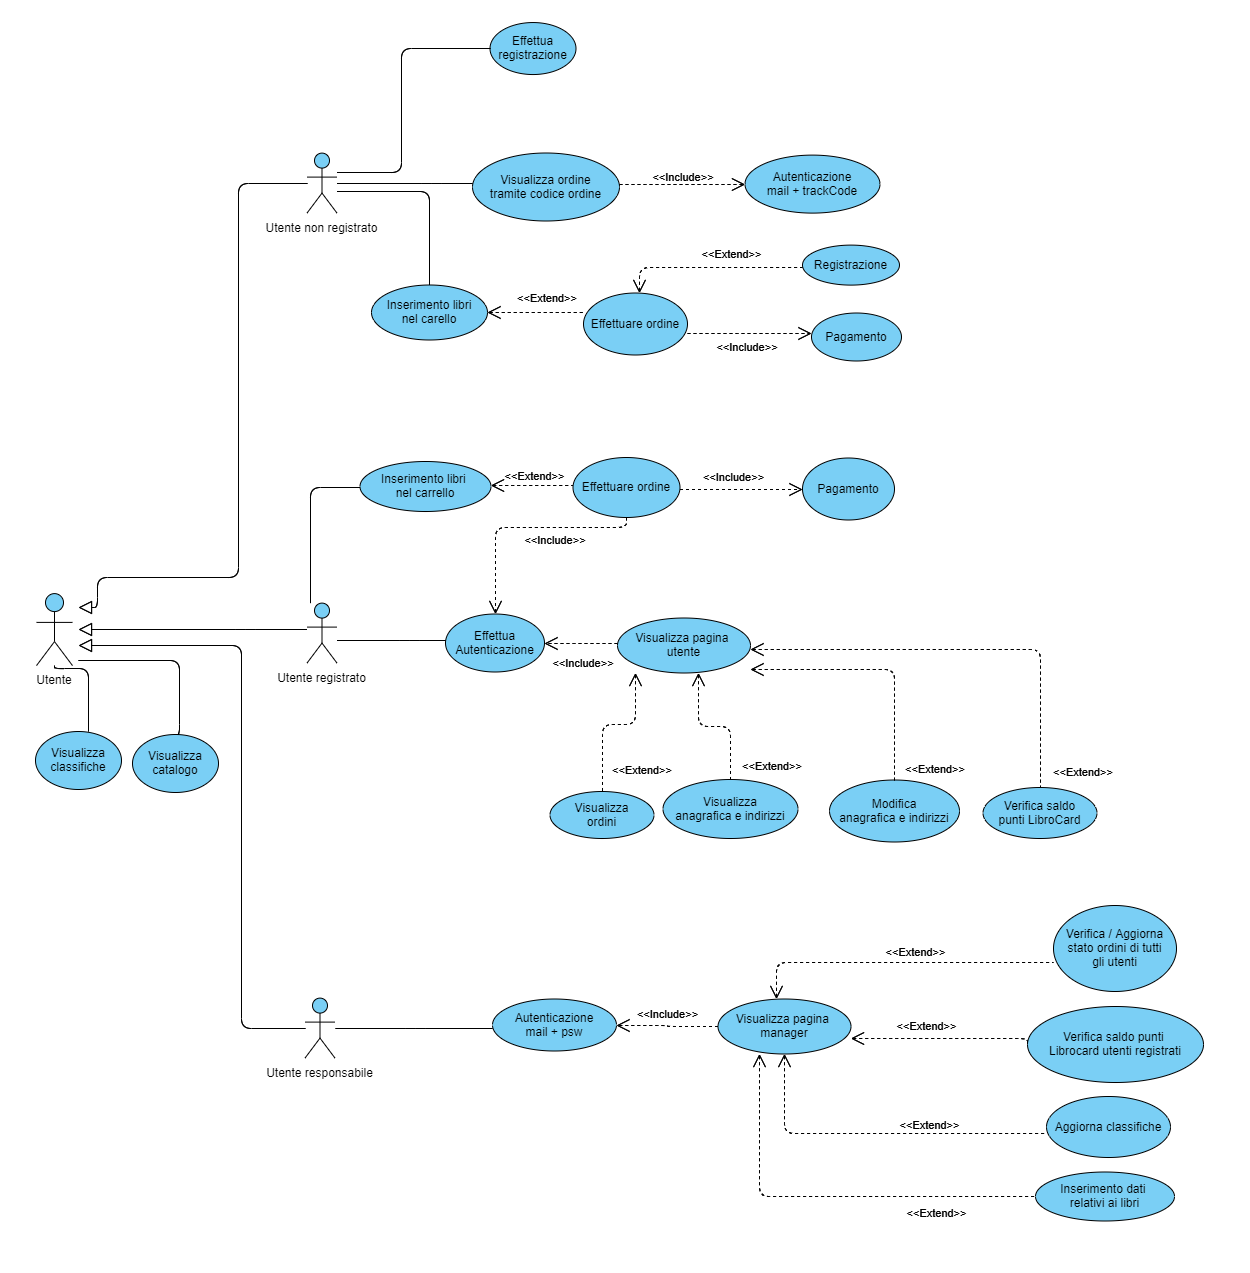
\includegraphics[width=1.1\linewidth]{Use cases diagrams/Use Case generale.png}
	\caption{Casi d'uso generale}
\end{figure}\\

\newpage
\subsection{Casi d'uso utente registrato}
Al fine di comprendere al meglio i casi d'uso di ogni singolo utente, viene di seguito riportata una descrizione maggiormente dettagliata circa le possibili interazioni con il sistema da parte di un utente registrato:
\begin{figure}[h!]
	\centering
	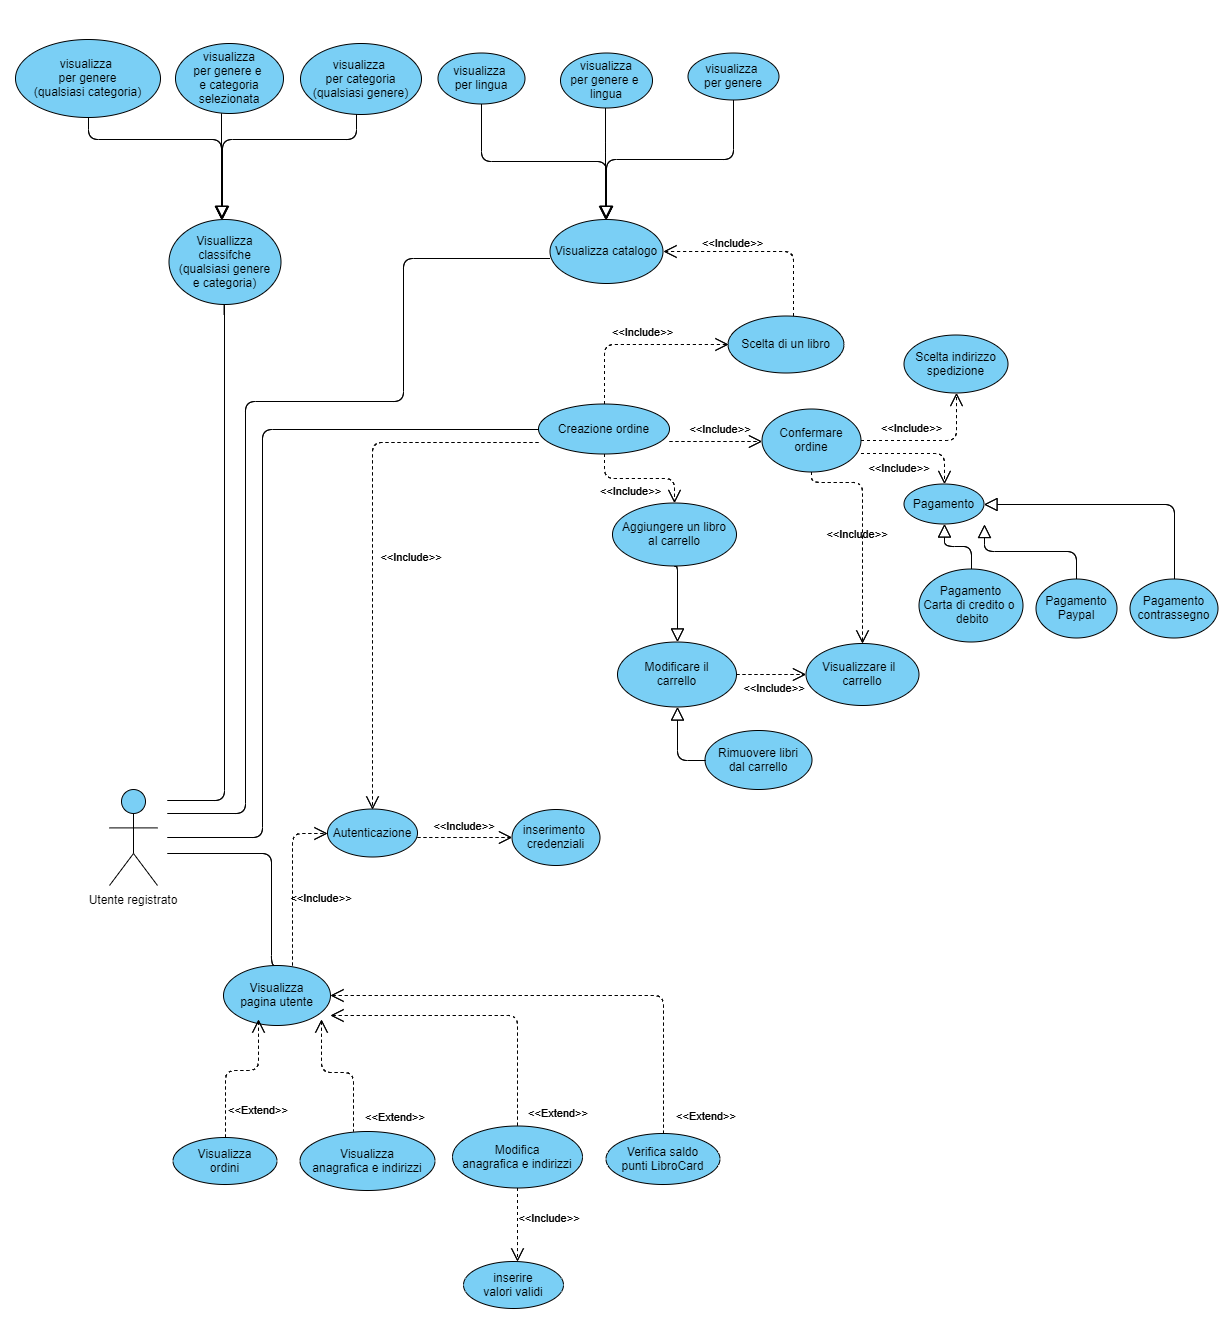
\includegraphics[width=1.1\linewidth]{Use cases diagrams/utente registrato.png}
	\caption{Casi d'uso utente registrato}
\end{figure}\\
Partendo dalle azioni che possono svolgere tutti gli utenti notiamo che anche l'utente registrato ha la possibilità di visionare le classifiche filtrandole, qualora lo volesse, per genere e/o categoria.\\
\newpage
L'utente registrato ha la possibilità di visionare il catalogo, anch'esso potenzialmente filtrato per genere e/o lingua.\\
Come presentato in precedenza notiamo inoltre che, dopo aver aggiunto libri al carrello e affinché l'utente registrato concluda un ordine, vi è la necessità che l'utente sia opportunamente autenticato dal sistema e successivamente che specifichi un indirizzo di spedizione e una modalità di pagamento valida.\\
L'utente registrato può inoltre accedere alla propria area personale previa autenticazione mediante mail e password.\\
Una volta effettuato l'accesso può visualizzare le proprie informazioni personali, modificare i propri dati anagrafici, visualizzare lo stato degli ordini e/o il saldo totale dei punti della LibroCard.

\subsection{Casi d'uso utente non registrato}
L'utente non registrato ha la possibilità di visionare il catalogo e le classifiche, potenzialmente filtrate qualora lo desiderasse.\\
Può inoltre creare un ordine e decidere se registrarsi o meno al sistema; in caso si registri deve necessariamente inserire tutte le informazioni necessarie al registrazioni quali dati anagrafici, mail univoca e password.\\
In caso invece voglia continuare come utente non registrato, viene chiesto comunque all'utente di inserire le proprio informazioni anagrafiche, una mail univoca e un indirizzo di spedizione valido. \\
\newline
L'utente non registrato può controllare lo stato degli ordini inserendo mail e tracking code dell'ordine.\\
Si rimanda alla prossima pagina per lo \textit{use case} completo:
\newpage
    \begin{figure}[h!]
    	\centering
    	\hspace*{-0.8in}
    	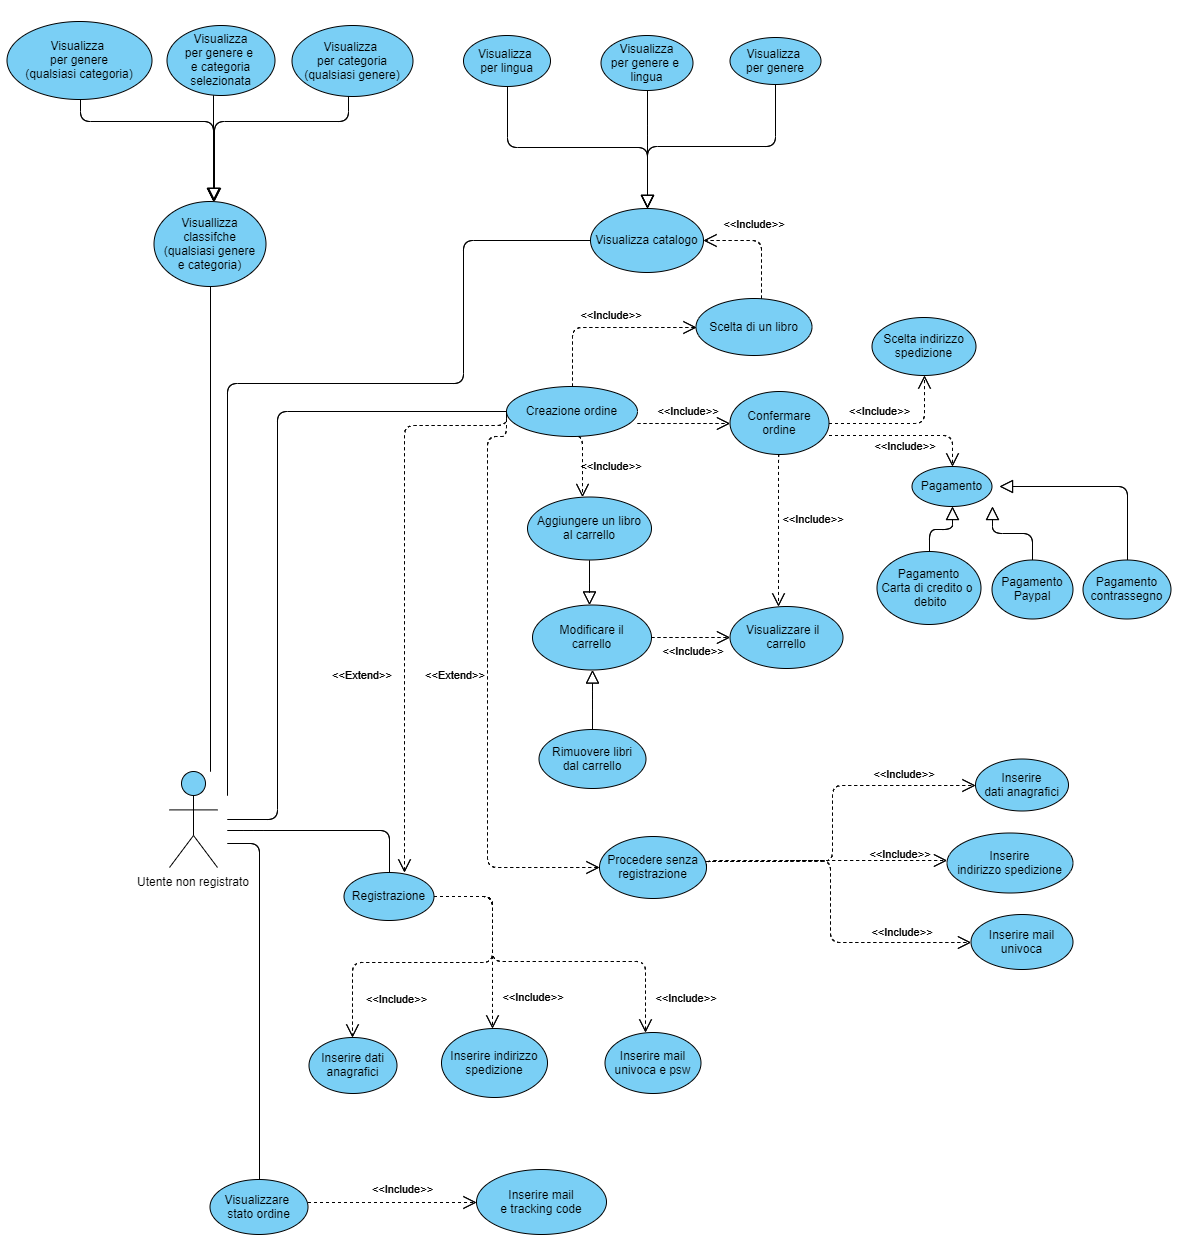
\includegraphics[width=1.3\linewidth]{Use cases diagrams/utente non registrato.png} 
    	\caption{Casi d'uso utente non registrato}
    \end{figure}
\newpage

\subsection{Casi d'uso utente responsabile}
L'utente responsabile può visualizzare classifiche e catalogo opportunamente filtrato qualora lo desiderasse; non può però effettuare acquisti.\\
Può accedere alla sua area personale previa autenticazione tramite mail e password e una volta effettuato l'accesso ha la possibilità di visualizzare lo stato degli ordini degli utenti registrati e non registrati, può aggiungere nuovi libri al catalogo o modificare libri già esistenti.\\
Infine l'utente responsabile può visualizzare il saldo relativo alle LibroCard degli utenti registrati.\\
L'utente responsabile inoltre può aggiornare le classifiche dei libri, scelte per categoria o genere o entrambi.\\
\vspace{2cm}

    \begin{figure}[h!]
    	\centering
    	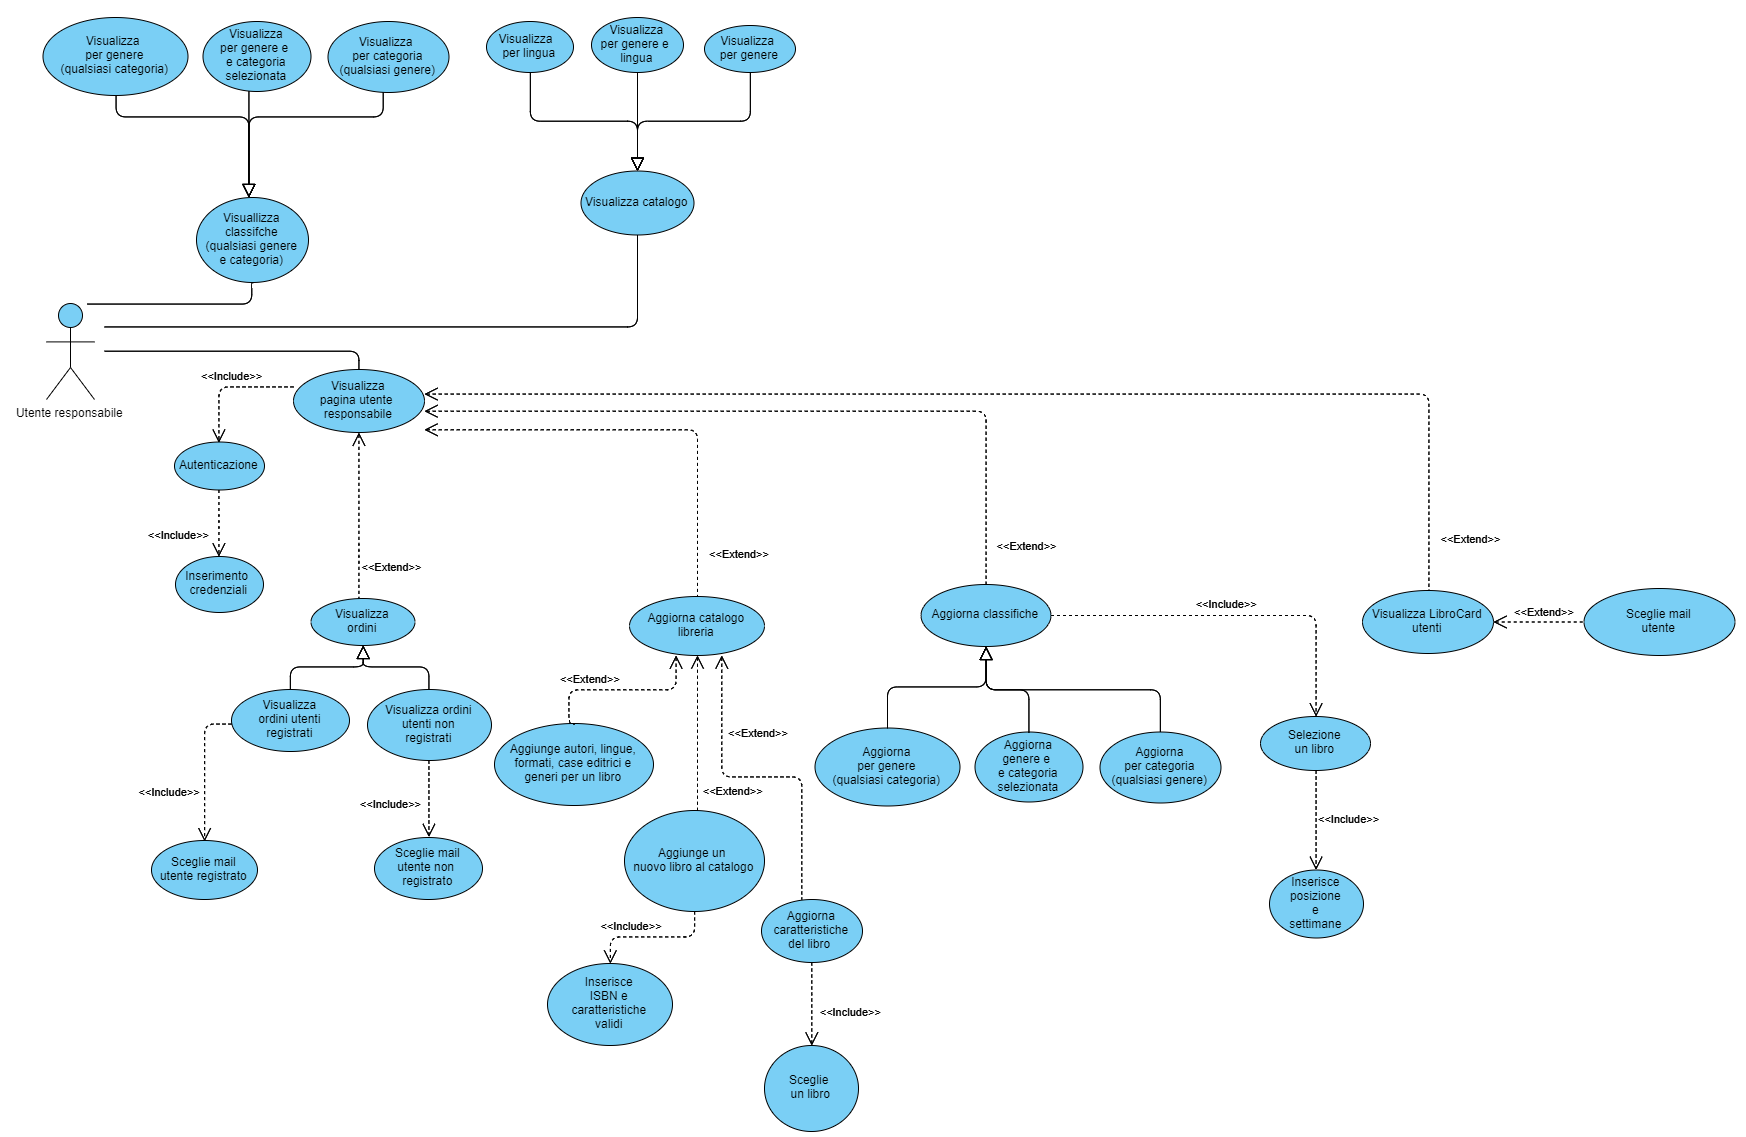
\includegraphics[width=1.2\linewidth]{Use cases diagrams/manager.png}
    	\caption{Casi d'uso utente responsabile}
    \end{figure}
%%%%%%%%%%%%%%%%%%%%%%%%%%%%%%%%%%%%%%%%%%%%%%%%%%%%%%%%%%%%%%%%%%%%%%%%%%%%%

\clearpage
\chapter{Schede di specifica dei casi d'uso}\label{spec casi d'uso}
Seguono ora una serie di schede di specifiche dei casi d'uso più dettagliati rispetto agli schemi sopra riportati:

\begin{table}[h!]
    \renewcommand*{\arraystretch}{1.2}
    \centering
    \begin{tabularx}{\textwidth}{|X|} \hline
      \textbf{ID}: Caso d'uso utente generico: 
      \newline 
      Visualizzazione classifiche \\
      \hline
      \textbf{ATTORI}: Utente generico \\
      \hline
      \textbf{PRECONDIZIONI}:\\
      \hline
      \textbf{SEQUENZA}:
      \begin{enumerate}
        \item L'utente cliccando sul bottone "Charts", ha la possibilità di vedere visionare le classifiche (generali di default).
        \begin{enumerate}
            \item [1.1] L'utente può filtrare le classifiche scegliendo il genere dall'apposito filtro.
            \item [1.2] L'utente ha la possibilità di filtrare le classifiche per categoria con l'apposito filtro.
             \item [1.3] L'utente ha la possibilità di filtrare le classifiche per genere e categoria selezionando entrambi i filtri dagli appositi menù a tendina.
         \end{enumerate}
      \end{enumerate}\\
      \hline
      \textbf{POSTCONDIZIONI}:
      \begin{enumerate}
        \item La schermata delle classifiche viene aggiornata in base ai filtri cliccati, se non si filtra rimane quella di default.
      \end{enumerate} \\
      \hline
    \end{tabularx}
  \end{table}
  
\clearpage

\begin{table}[h!]
    \renewcommand*{\arraystretch}{1.2}
    \centering
    \begin{tabularx}{\textwidth}{|X|} \hline
      \textbf{ID}: Caso d'uso utente registrato: 
      \newline 
      Pagina personale utente registrato e modifica indirizzi di spedizione \\
      \hline
      \textbf{ATTORI}: Utente registrato \\
      \hline
      \textbf{PRECONDIZIONI}:
      \begin{enumerate}
        \item L'Utente deve essersi autenticato con le proprie credenziali.
      \end{enumerate} \\
      \hline
      \textbf{SEQUENZA}:
      \begin{enumerate}
        \item L'utente cliccando sul bottone "My Orders", ha la possibilità di vedere lo stato di tutti i suoi ordini.
        
        \item L'utente cliccando sul bottone "My LibroCard", ha la possibilità di verificare il saldo attuale dei punti della sua LibroCard
      \end{enumerate} \\
      \hline
      \textbf{POSTCONDIZIONI}:
      \begin{enumerate}
        \item In caso l'utente modifichi i suoi dati anagrafici, i valori vengono raccolti dal sistema e viene aggiornato il DB con le nuove informazioni.
      \end{enumerate} \\
      \hline 
    \end{tabularx}
  \end{table}  

\begin{table}[h!]
    \renewcommand*{\arraystretch}{1.2}
    \centering
    \begin{tabularx}{\textwidth}{|X|} \hline
      \textbf{ID}: Caso d'uso generale: \\ Creazione Ordine \\
      \hline
      \textbf{ATTORI}: Utente registrato o Utente non registrato \\
      \hline
      \textbf{PRECONDIZIONI}:
      \begin{enumerate}
        \item L'Utente ha consultato il catalogo, eventualmente filtrandolo per genere e/o lingua.
        \item L'utente ha inserito nel carrello almeno un libro.
      \end{enumerate} \\
      \hline
      \textbf{SEQUENZA}:
      \begin{enumerate}
        \item L'utente clicca sul bottone del carrello e viene indirizzato alla pagine del carrello contenente i libri scelti.
        \newline
        \item Quando l'utente clicca sul bottone "Proceed to CheckOut": 
        \begin{itemize}
          \item [a.] Se l'utente è registrato e ha già effettuato l'autenticazione, il sistema lo porta alla schermata di pagamento, dove dopo avere selezionato un indirizzo di spedizione e un metodo di pagamento valido, l'ordine si conclude.
          \newline
          \item [b.] Se l'utente è registrato ma non ha ancora effettuato l'accesso, il sistema lo porta alla schermata di login, dove dopo aver inserito le proprie credenziali, prosegue come al punto [a].
           \newline
          \item [c.] Se l'utente non è  registrato, allora il sistema lo porta alla schermata di Login-SignUp, dove l'utente può decidere o di registrarsi o di proseguire come utente non registrato:
          \begin{itemize}
              \item [c.1] se l'utente decide di registrarsi,viene portato alla schermata di registrazione e dopo avere inserito i dati per la registrazione si prosegue con [a].
              \newline
              \item [c.2] se l'utente decide di proseguire senza registrazione viene condotto ad una pagina dove inserire le sue informazioni personali, indirizzo di spedizione e una mail univoca per associare l'ordine, se i campi inseriti sono validi allora il sistema lo aggiunge al DB e poi si prosegue con [a].
          \end{itemize}
        \end{itemize}
      \end{enumerate} \\
      \hline
      \textbf{POSTCONDIZIONI}:
      \begin{enumerate}
        \item L'ordine viene creato e inserito nel DB associato a quel determinato utente.
      \end{enumerate} \\
      \hline
    \end{tabularx}
  \end{table}
  
 
  
  \begin{table}[h!]
    \renewcommand*{\arraystretch}{1.2}
    \centering
    \begin{tabularx}{\textwidth}{|X|} \hline
      \textbf{ID}: Caso d'uso utente non registrato: \\Registrazione\\
      \hline
      \textbf{ATTORI}: Utente non registrato \\
      \hline
      \textbf{PRECONDIZIONI}:
      \begin{enumerate}
        \item L'Utente non deve essere registrato e deve usare per la registrazione una mail diversa da quella usata per un eventuale precedente acquisto come non registrato.
      \end{enumerate} \\
      \hline
      \textbf{SEQUENZA}:
      \begin{enumerate}
        \item L'utente cliccando sul bottone "Login-SignUp", viene portato dal sistema alla pagina di accesso o registrazione.
        \newline
        \item L'utente cliccando sul bottone "SignUp", viene condotto alla schermata di registrazione.
        \newline
        \item Qui inserisce tutti i dati anagrafici, un indirizzo valido e un mail univoca e password.
        \newline
        \item L'utente poi clicca sul bottone "SignUp":
        \begin{enumerate}
            \item [3.1] Il sistema dopo che l'utente ha inserito i dati anagrafici e mail, verifica che i valori siano validi, ovvero che i campi rispettino le richieste e che la mail sia univoca. 
            \newline
            \item [3.2] In caso non siano validi il sistema avvisa l'utente e si ritorna al punto [3.1].
        \end{enumerate}
        \item Se tutto è corretto l'utente cliccando sul bottone "SignUp" si registra al sistema.
      \end{enumerate} \\
      \hline
      \textbf{POSTCONDIZIONI}:
      \begin{enumerate}
        \item L'utente viene inserito nel DB.
      \end{enumerate} \\
      \hline
    \end{tabularx}
  \end{table}
  
  \clearpage
  
  
   \begin{table}[h!]
    \renewcommand*{\arraystretch}{1.2}
    \centering
    \begin{tabularx}{\textwidth}{|X|} \hline
      \textbf{ID}: Caso d'uso utente responsabile: \\Visualizzazione ordine e inserimento o modifica di un libro\\
      \hline
      \textbf{ATTORI}: Utente responsabile \\
      \hline
      \textbf{PRECONDIZIONI}:
      \begin{enumerate}
        \item L'Utente responsabile deve essersi autenticato con le proprie credenziali.
      \end{enumerate} \\
      \hline
      \textbf{SEQUENZA}:
      \begin{enumerate}
        \item L'utente responsabile cliccando sul bottone "View Order Status" ha la possibilità di vedere lo stato degli ordini di tutti gli utenti (default):
        \begin{enumerate}
            \item [1.1] Ha la possibilità inoltre di filtrare gli ordini per utenti registrati e non registrati da un apposito filtro
            \item [1.2] L'utente responsabile ha la possibilità di modificare lo stato degli ordini tramite un apposito menù a tendina.
            \item [1.3] Qualora il responsabile modificasse lo stato di un ordine compare un messaggio che lo informa che stato dell'ordine è stato cambiato.
        \end{enumerate}
        \item L'utente responsabile cliccando sul bottone "Add/Edit book", ha la possibilità di aggiungere autori, generi, formati, lingue e case editrici ognuna di queste in un apposita schermata, oppure aggiungere direttamente un nuovo libro cliccando su "Add new book" che porta in una schermata apposita. 
        \item L'utente può anche modificare un libro già esistente, andando a modificare i singoli campi che compongono il libro, cliccando sul bottone "Edit Book".
        \begin{enumerate}
            \item [3.1] Dopo che l'utente ha inserito i dati relativi ai libri, sia che sia un nuovo libro o una modifica e dopo aver cliccato rispettivamente sul bottone "Add new book" o "Edit book", il sistema verifica che i valori siano validi, ovvero che i campi rispettino le richieste. 
            \item [3.2] In caso non siano validi il sistema avvisa l'utente e si ritorna al punto [3.1].
        \end{enumerate}
      \end{enumerate} \\
      \hline
      \textbf{POSTCONDIZIONI}:
      \begin{enumerate}
        \item In caso di modifica dello stato dell'ordine viene aggiornata l'informazione nel DB. 
        \item Il libro viene aggiornato nel DB (in caso di Edit).
        \item Il libro viene inserito nel DB (in caso di Add).
      \end{enumerate} \\
      \hline
    \end{tabularx}
  \end{table}
  \clearpage
  
  \begin{table}[h!]
    \renewcommand*{\arraystretch}{1.2}
    \centering
    \begin{tabularx}{\textwidth}{|X|} \hline
      \textbf{ID}: Caso d'uso utente responsabile: \\Aggiornamento delle classifiche\\
      \hline
      \textbf{ATTORI}: Utente responsabile \\
      \hline
      \textbf{PRECONDIZIONI}:
      \begin{enumerate}
        \item L'Utente responsabile deve essersi autenticato con le proprie credenziali.
      \end{enumerate} \\
      \hline
      \textbf{SEQUENZA}:
      \begin{enumerate}
        \item L'utente responsabile cliccando sul bottone "Update Charts" ha la possibilità di aggiornare le classifiche:
        \begin{enumerate}
            \item [1.1] Ha la possibilità di filtrare le classifiche da aggiornare per genere dei libri e/o categoria.
            \item [1.2] Oppure può aggiornare la classifica inerente a qualsiasi genere e categoria, una sorta di classifica assoluta.
            \begin{itemize}
                \item Per inserire un libro in classifica è necessario indicare la posizione dove si vuole inserire e da quante settimane è in classifica.
            \end{itemize}
            \item [1.3] Cliccando sul bottone "Insert/Edit book in Charts" l'utente può inserire o aggiornare un libro nella classifica selezionata.
            \begin{itemize}
                \item Il sistema dopo che l'utente ha cliccato sul bottone verifica che i campi (posizione e settimane) siano riempiti correttamente e in caso contrario avvisa l'utente.
            \end{itemize}
            \item [1.4] Cliccando sul bottone "Delete book from Charts" l'utente può rimuovere un libro dalla classifica selezionata.
            \begin{itemize}
                \item Il sistema dopo che l'utente ha cliccato sul bottone verifica che i campi (posizione e settimane) siano riempiti correttamente e in caso contrario avvisa l'utente.
            \end{itemize}             
        \end{enumerate}
      \end{enumerate} \\
      \hline
      \textbf{POSTCONDIZIONI}:
      \begin{enumerate}
        \item La classifica viene aggiornata anche sul DB.
      \end{enumerate} \\
      \hline
    \end{tabularx}
  \end{table}
\clearpage

%%%%%%%%%%%%%%%%%%%%%%%%%%%%%%%%%%%%%%%%%%%%%%%%%%%%%%%%%%%%%%%%%%%%%%%%%

\chapter{Diagramma delle sequenze}
Vengono presentati di seguito i principali diagrammi delle sequenze dei casi d'uso presentati al paragrafo \ref{spec casi d'uso}.\\
Si precisa che alcuni di questi diagrammi di sequenza qui presentati sono stati semplificati per un discorso di chiarezza e leggerezza; si considerano quindi le singole sequenze contenti le chiamate ai metodi principali. \\
\newline
Partiamo con il diagramma di sequenza inerente alla visualizzazione del catalogo da parte di un \underline{utente generico}:
\begin{figure}[h!]
    	\centering
    	\hspace*{-0.4in}
    	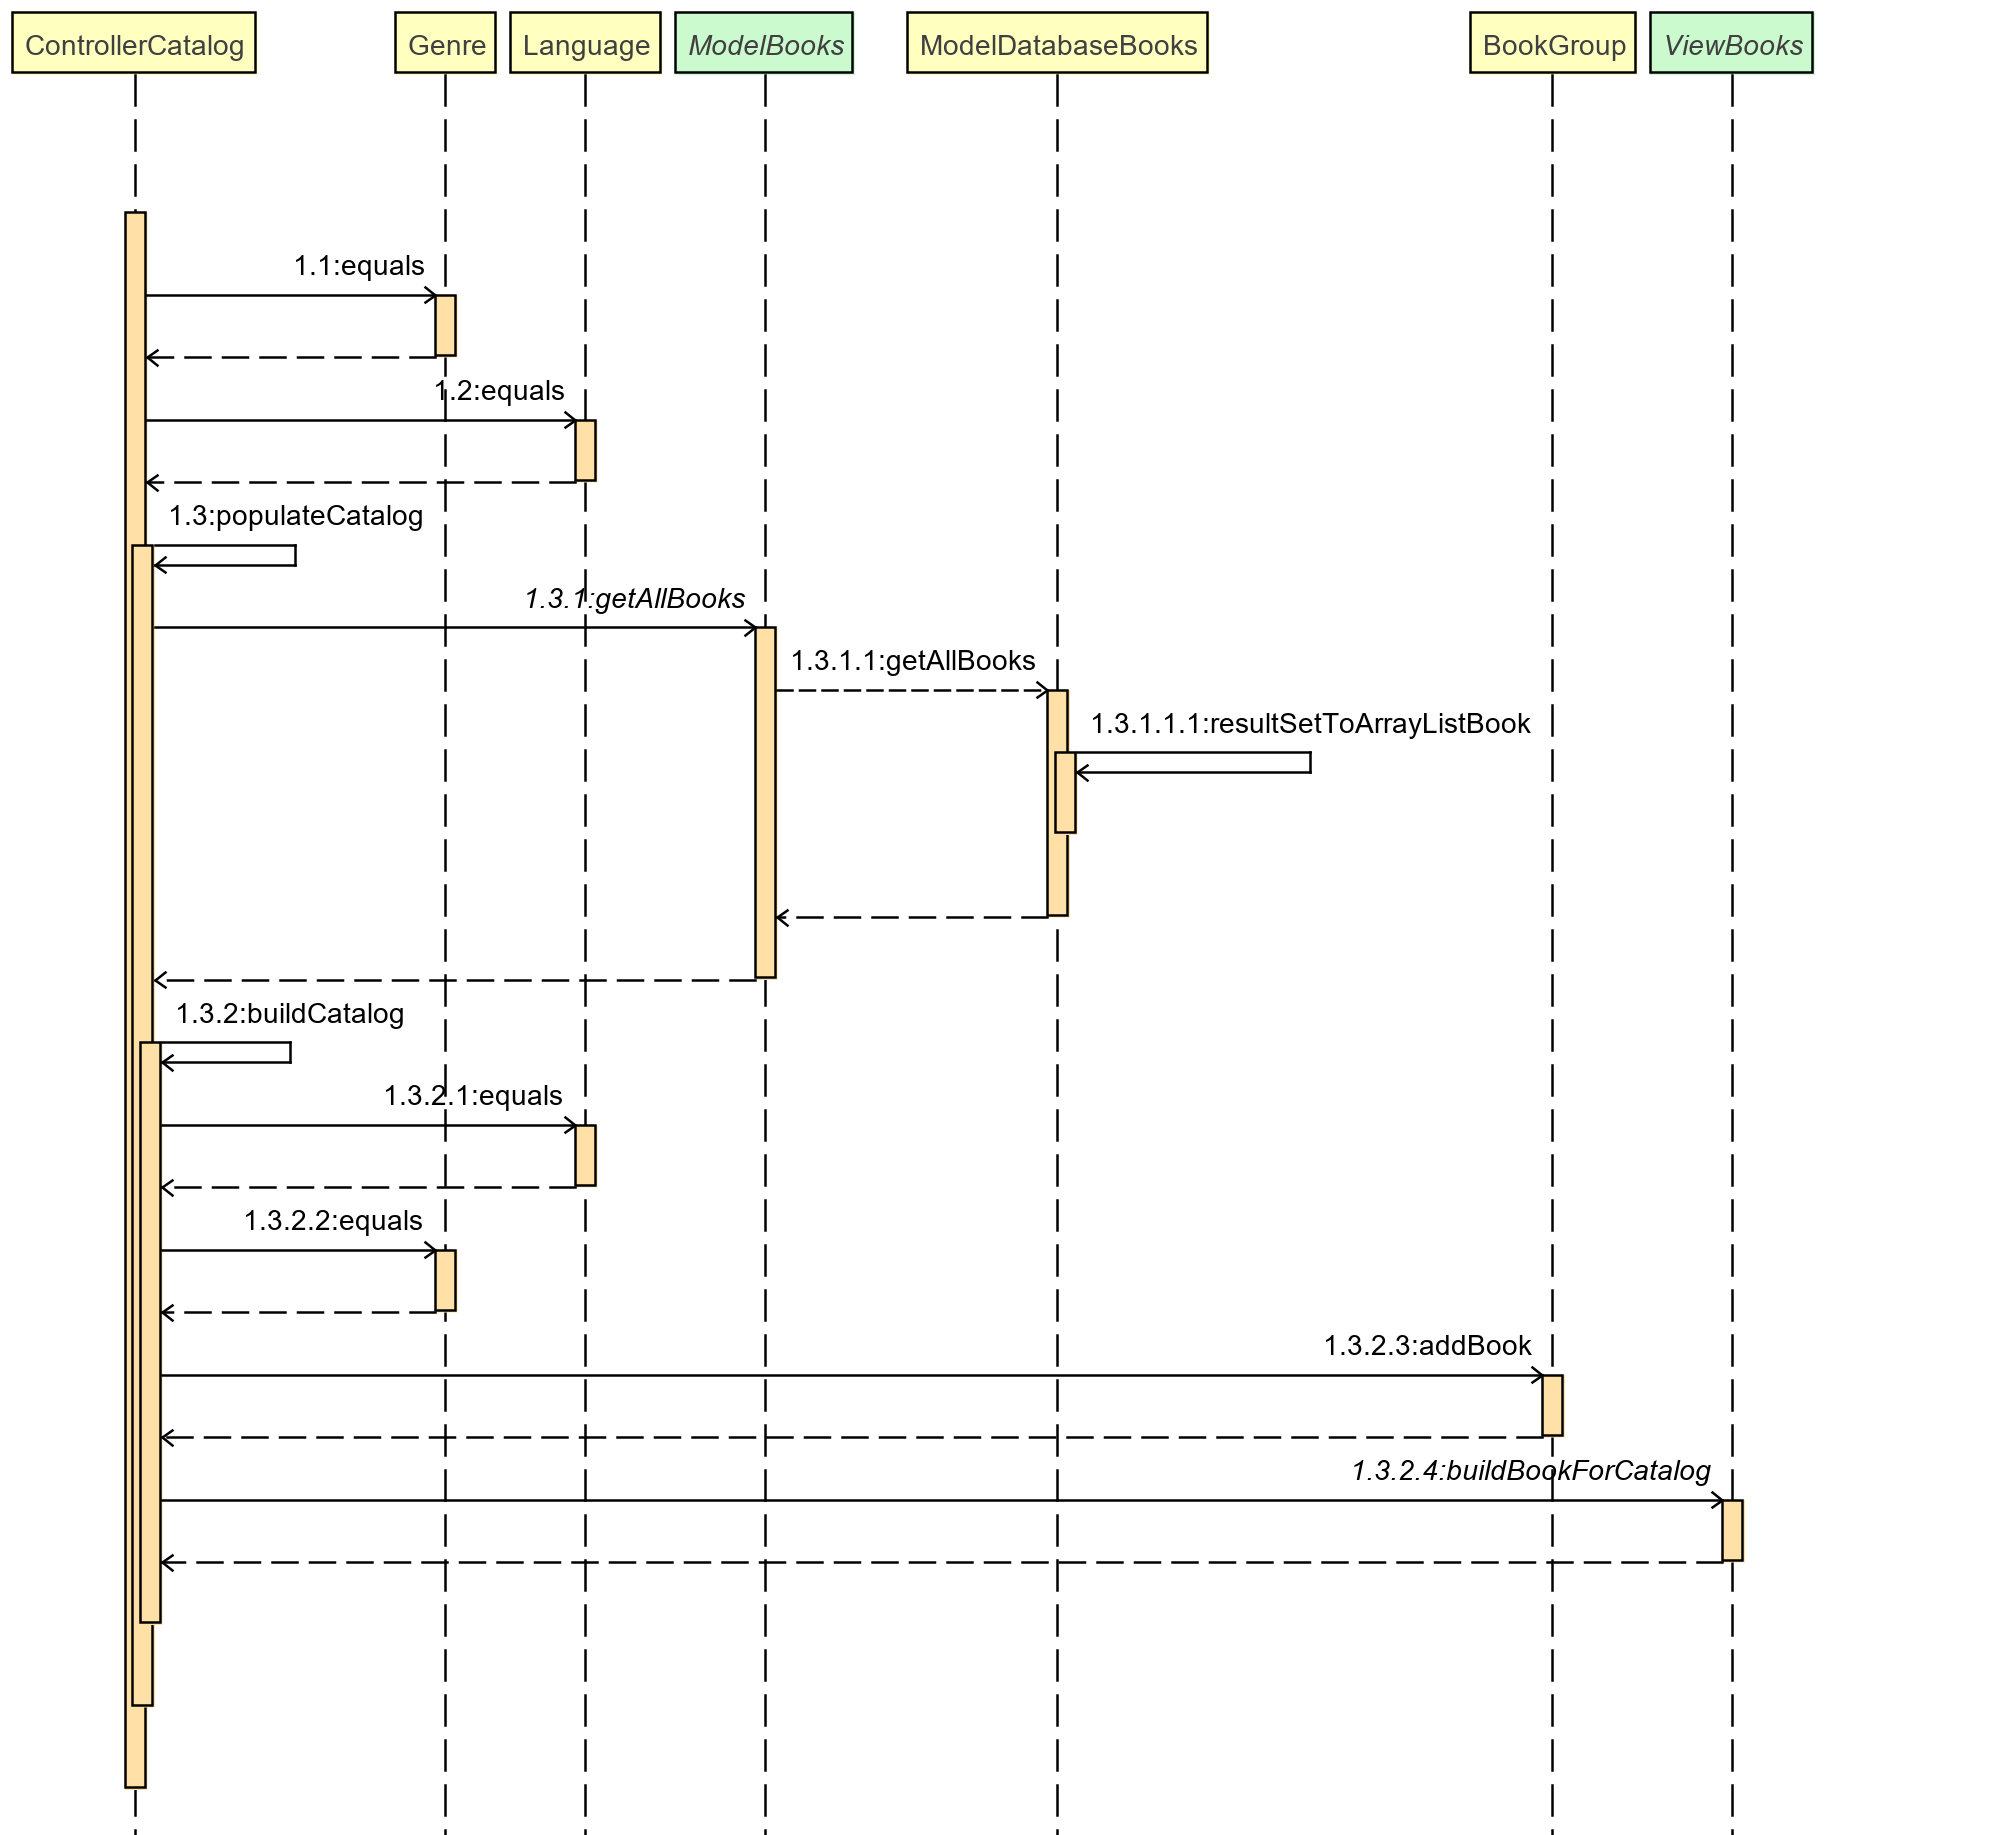
\includegraphics[width=1.2\linewidth]{Sequence diagrams/2 Order Creation/ViewCatalog.png}
    	\caption{Diagramma sequenza visualizza catalogo utente generico}
    \end{figure}\\
    
\clearpage

Viene di seguito riportato il diagramma di sequenza per la visione delle classifiche per \underline{l'utente generico}:\\
\begin{figure}[h!]
    	\centering
    	\hspace*{-0.4in}
    	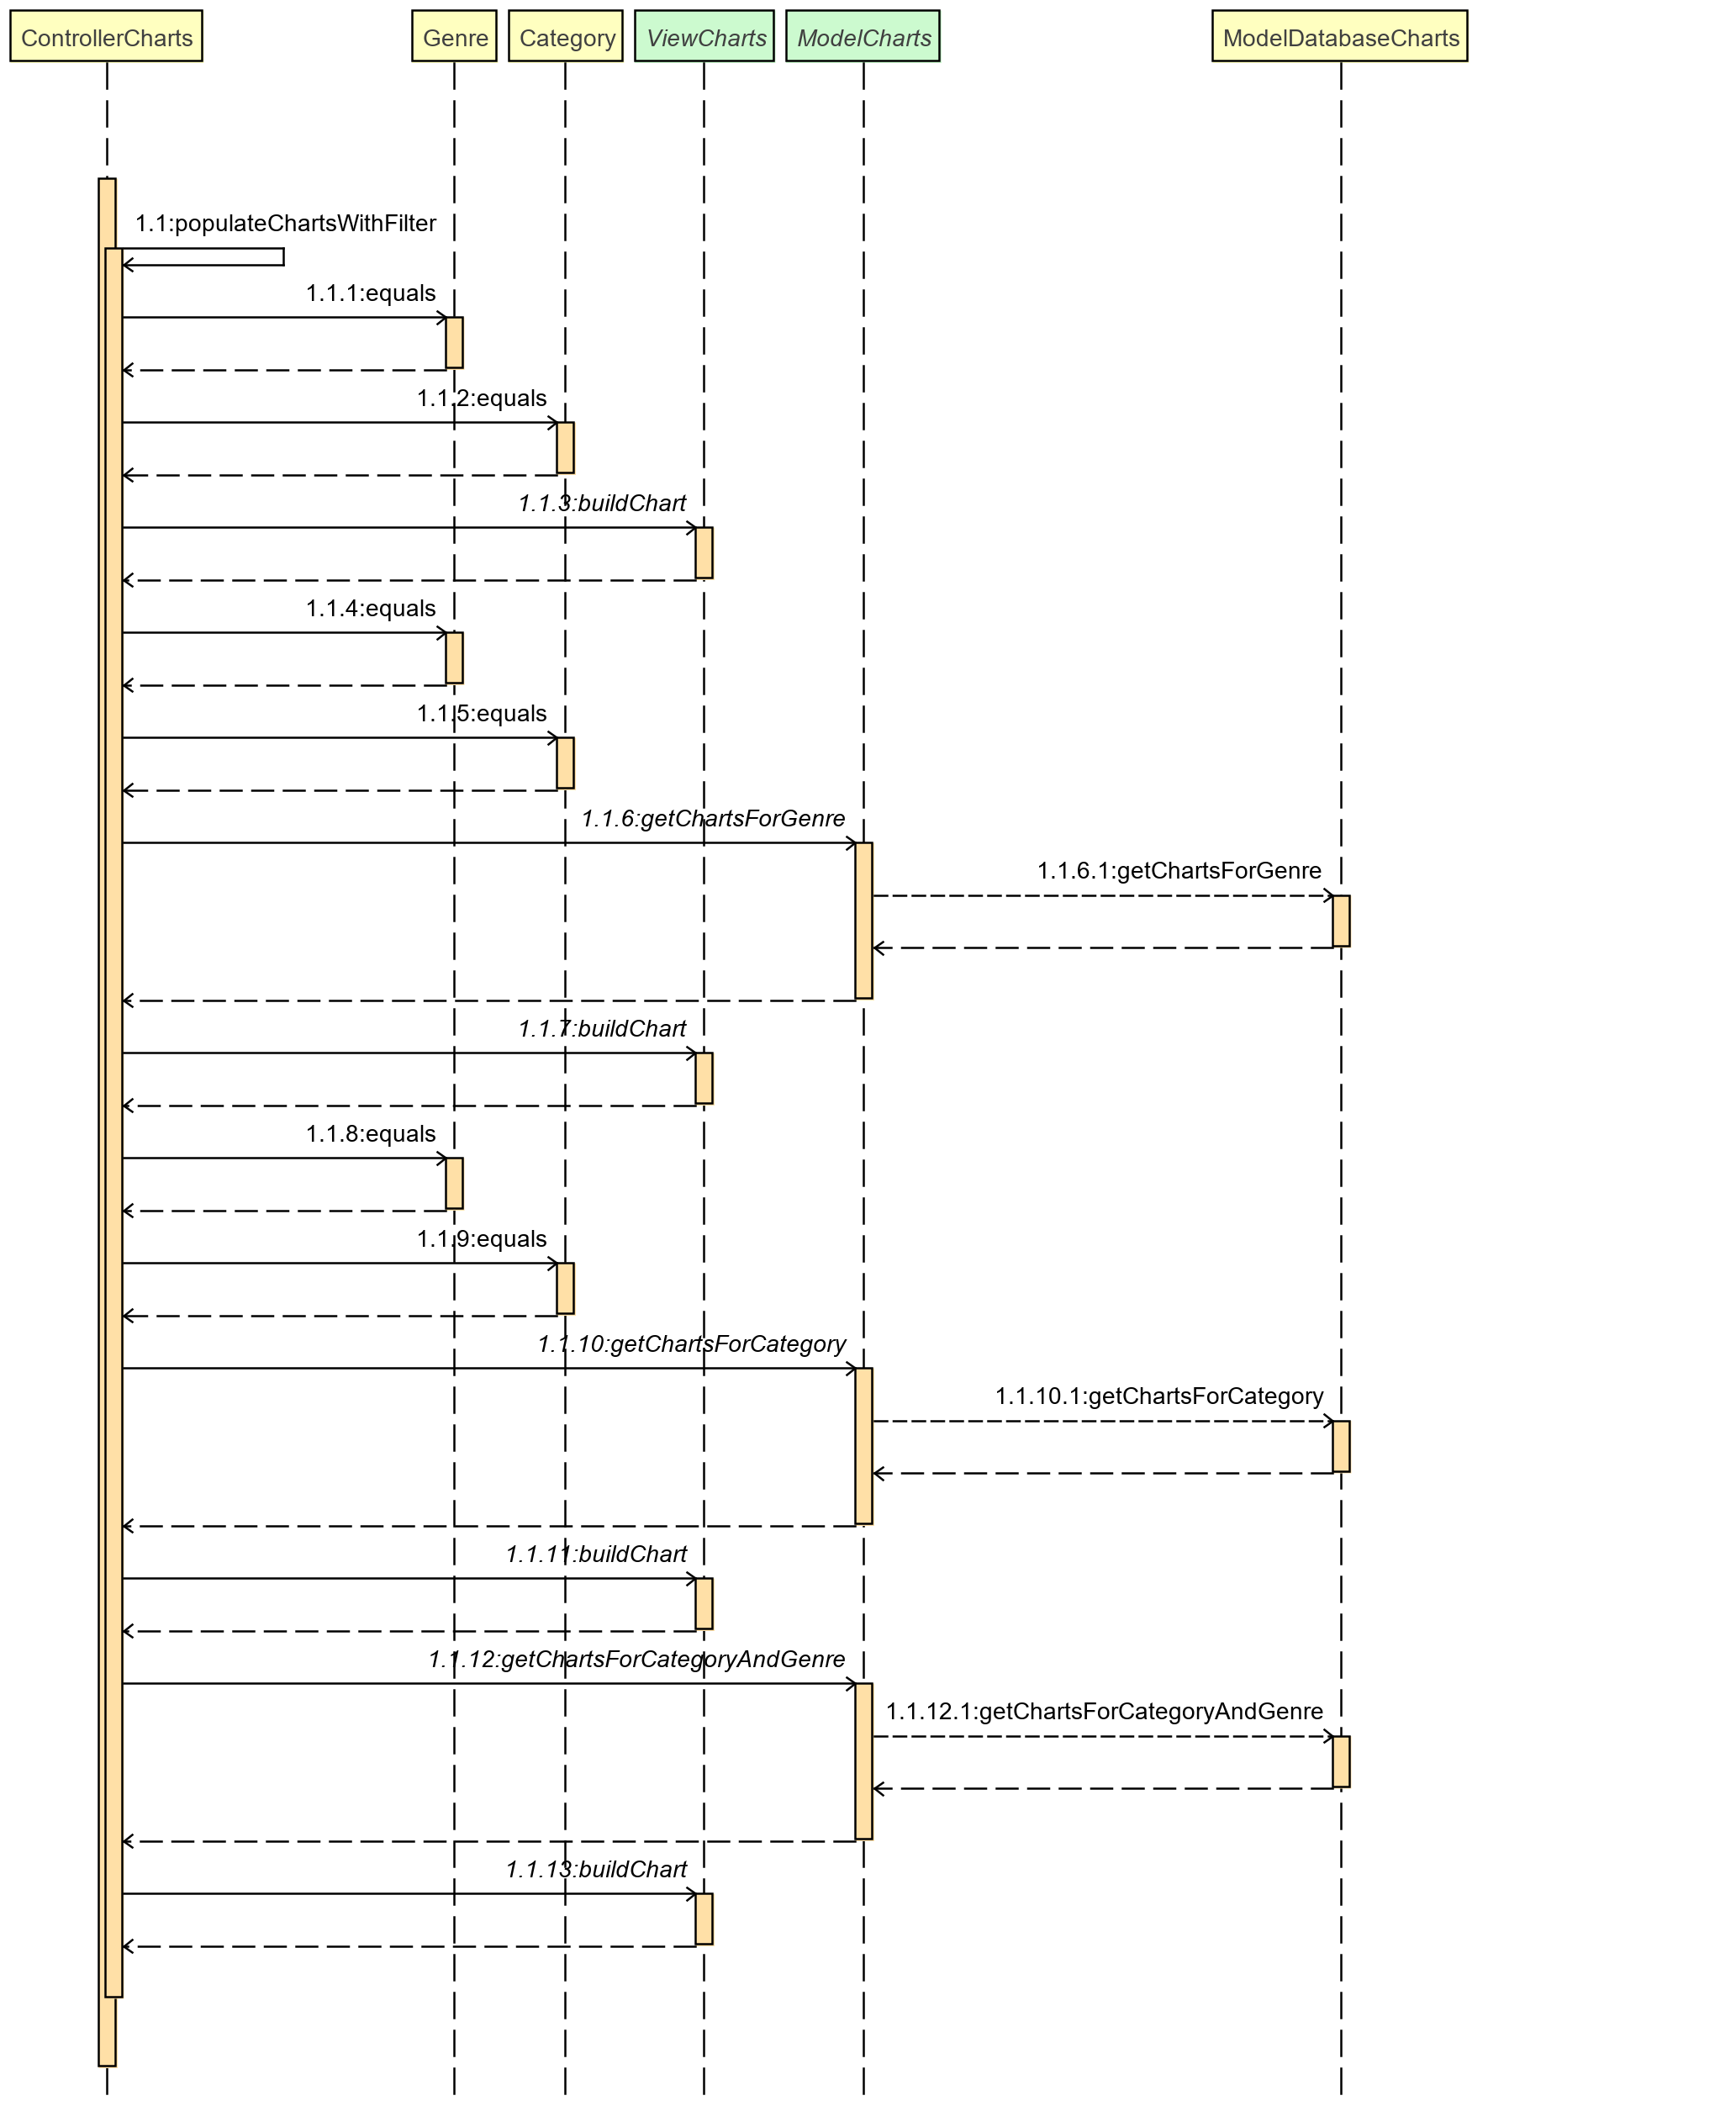
\includegraphics[width=1.1\linewidth]{Sequence diagrams/2 Order Creation/viewCharts.png}
    	\caption{Diagramma sequenza visualizza classifiche utente generico}
    \end{figure}\\
\clearpage

\leavevmode \newline
Iniziamo a vedere il diagramma delle sequenze inerente \underline{all'utente registrato} e in particolare la \textbf{modifica dei dati anagrafici}:\\
Per quanto riguarda la spiegazione di classi, interfacce e pattern utilizzati si rimanda al capitolo inerente alle scelte progettuali e allo sviluppo.\\
Definiamo qui di seguito però alcune caratteristiche importanti implementante al fine di rispettare i requisiti. L'utente dopo essersi opportunamente autentico può accedere tramite il bottone "Edit Profile" alla pagine per modificare i propri dati anagrafici.\\
\newline
Qui l'utente ha la possibilità di modificare i propri dati anagrafici, aggiungere e/o rimuovere indirizzi di spedizione.
\newline
Nel diagramma di sequenza, presentato nella prossima pagina, siamo voluti andare ad un livello di dettaglio maggiore al fine di mostrare la comunicazione tra sistema e DB nel caso di aggiornamento di indirizzi da parte dell'utente registrato.\\

\leavevmode \newline
Lo schema è stato inserito nella prossima pagina per questioni di spazio.\\

\clearpage

\begin{figure}[h!]
    	\centering
    	\hspace*{-0.4in}
    	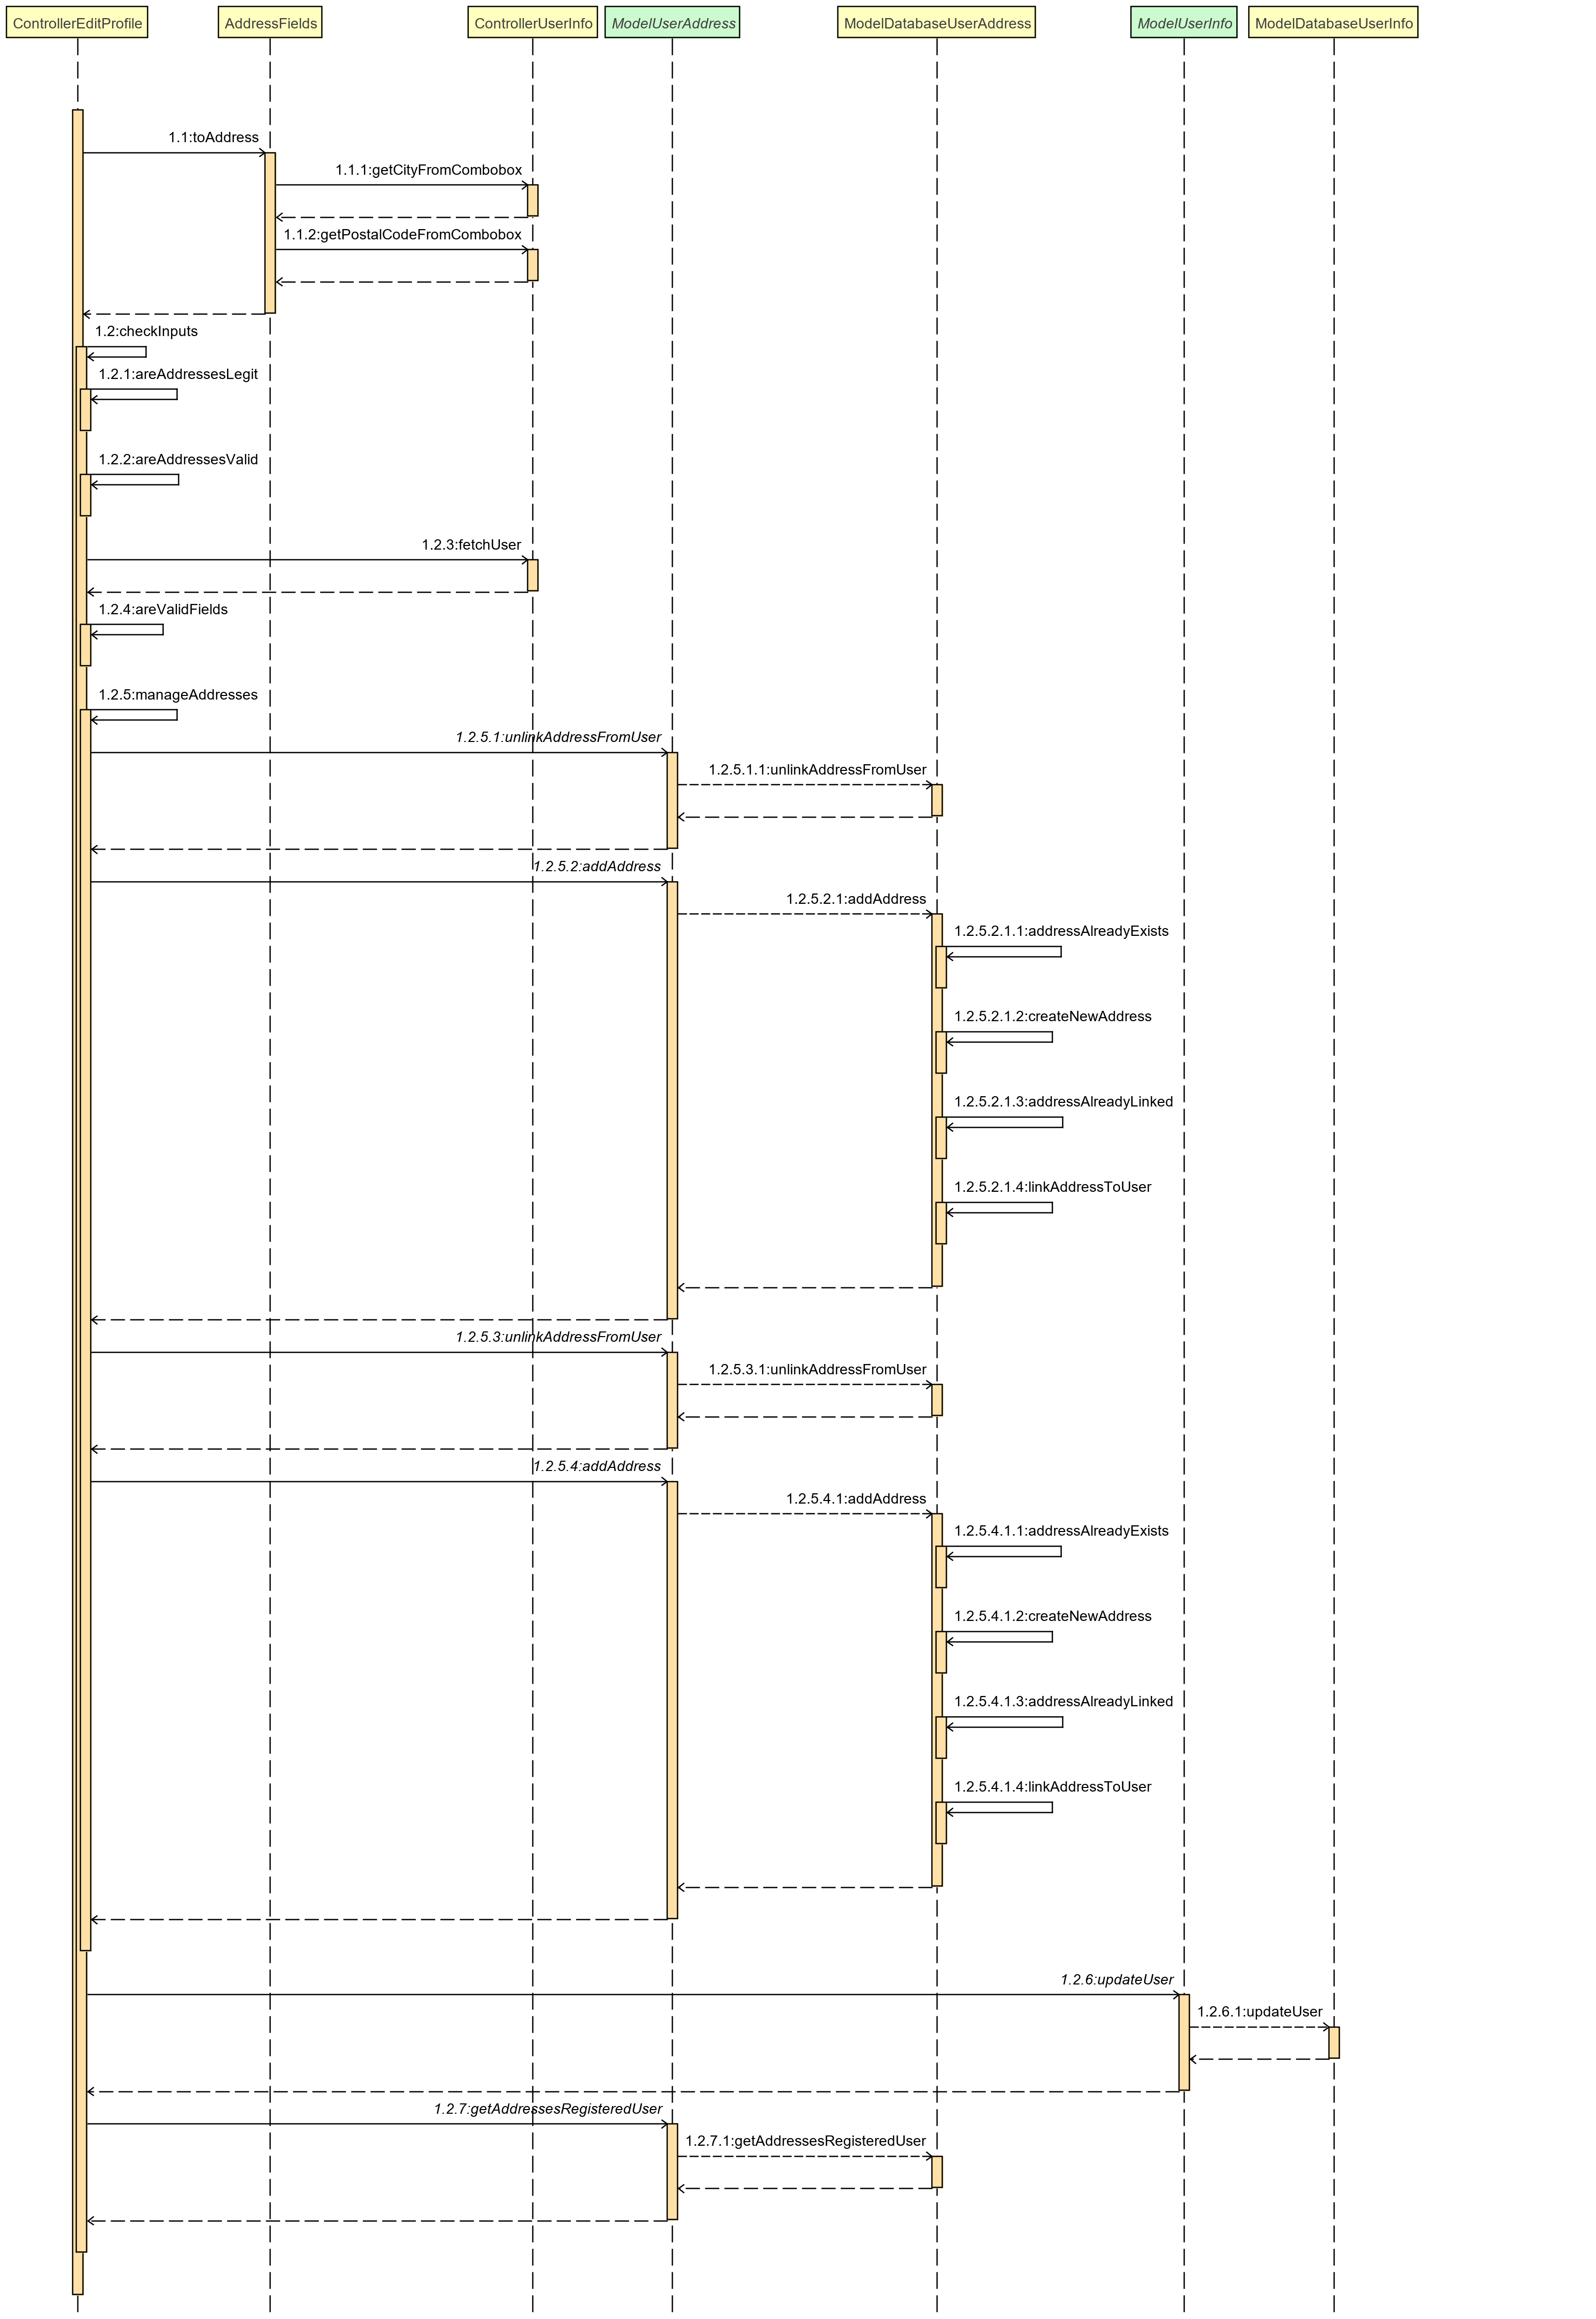
\includegraphics[width=1.0\linewidth]{Sequence diagrams/1 Registered user/updateProfile.png}
    	\caption{Diagramma sequenza modifica dati anagrafici utente registrato}
    \end{figure} \leavevmode \\

I prossimi diagrammi delle sequenze che presentiamo sono sempre inerenti \underline{all'utente registrato} e in ordine riguardano:
\begin{itemize}
    \item Visione del profilo personale
    \item Visione di tutti gli ordini effettuati
    \item Visione del saldo punti inerenti alla LibroCard
\end{itemize}
\leavevmode \newline
\vspace{1in}
   \begin{figure}[h!]
    	\centering
    	\hspace*{-0.4in}
    	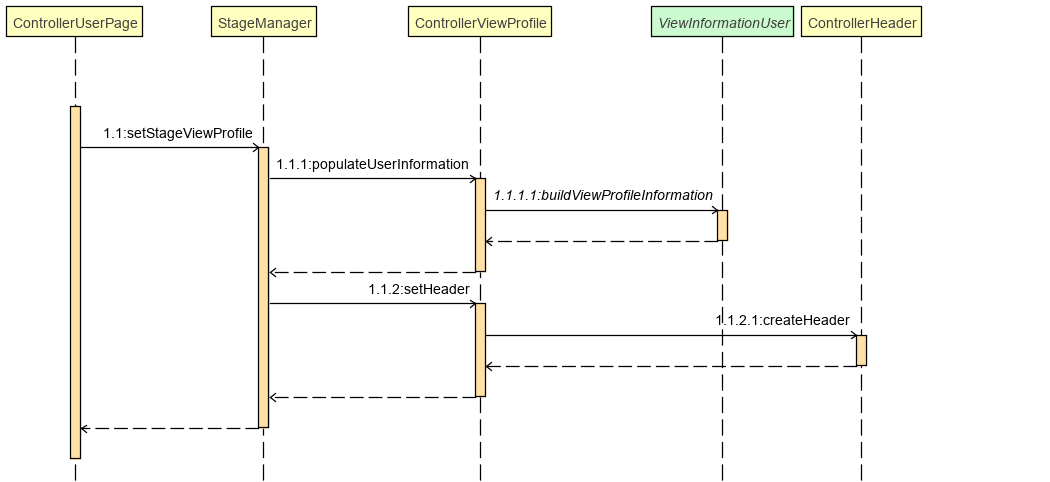
\includegraphics[width=1.3\linewidth]{Sequence diagrams/1 Registered user/UserViewProfile.png}
    	\caption{Diagramma sequenza visualizza profilo utente registrato}
    \end{figure}\leavevmode  \\
\clearpage
     \begin{figure}[h!]
    	\centering
    	\hspace*{-0.4in}
    	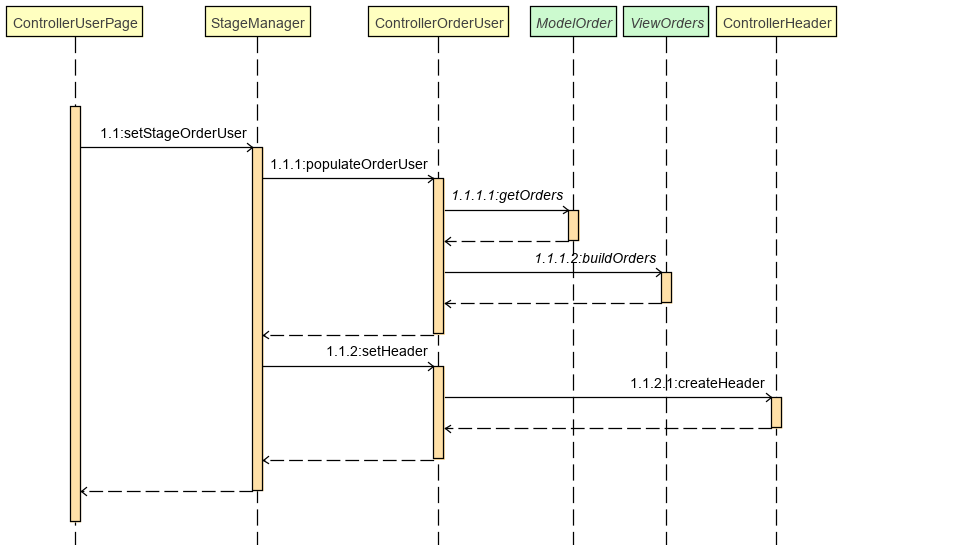
\includegraphics[width=1.3\linewidth]{Sequence diagrams/1 Registered user/UserMyOrders.png}
    	\caption{Diagramma sequenza visualizza ordini effettuati utente registrato}
    \end{figure} \leavevmode \\
    
     \begin{figure}[h!]
    	\centering
    	\hspace*{-0.4in}
    	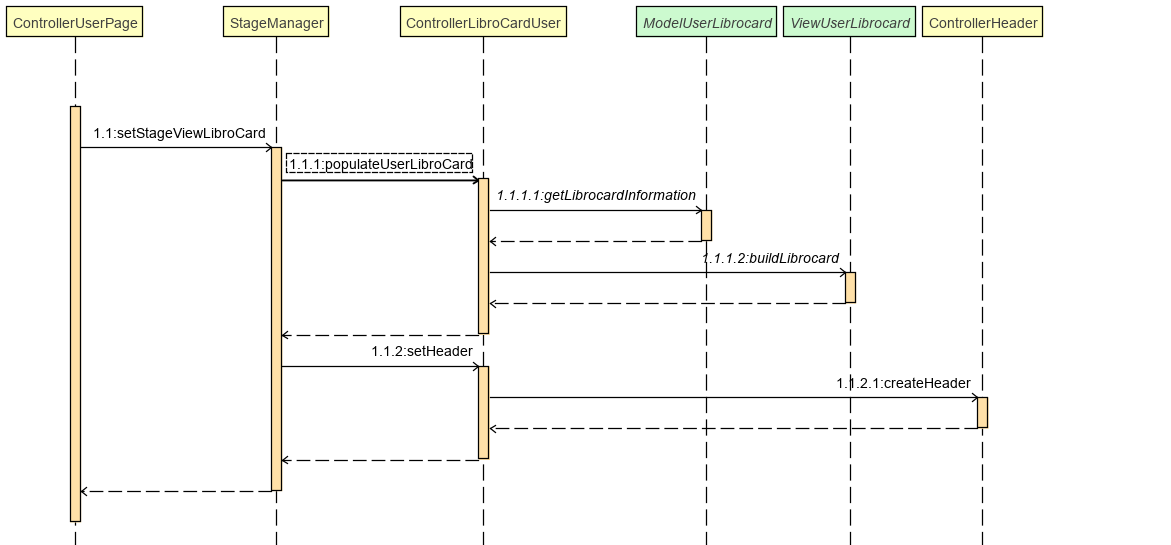
\includegraphics[width=1.3\linewidth]{Sequence diagrams/1 Registered user/UserLibrocard.png}
    	\caption{Diagramma sequenza visualizza LibroCard utente registrato}
    \end{figure}
\clearpage
 I prossimi diagrammi delle sequenze riguardano invece la \textbf{creazione dell'ordine} da parte di \underline{utenti registrati} o \underline{utenti non registrati}.
\newline
Abbiamo detto in precedenza (nello use case per la creazione dell'ordine) che è necessario prima cliccare sul carrello e visualizzare il riepilogo dei libri scelti. Presentiamo quindi di seguito cosa succede quando l'utente clicca sull'immagine del carrello:\\
 \begin{figure}[h!]
    	\centering
    	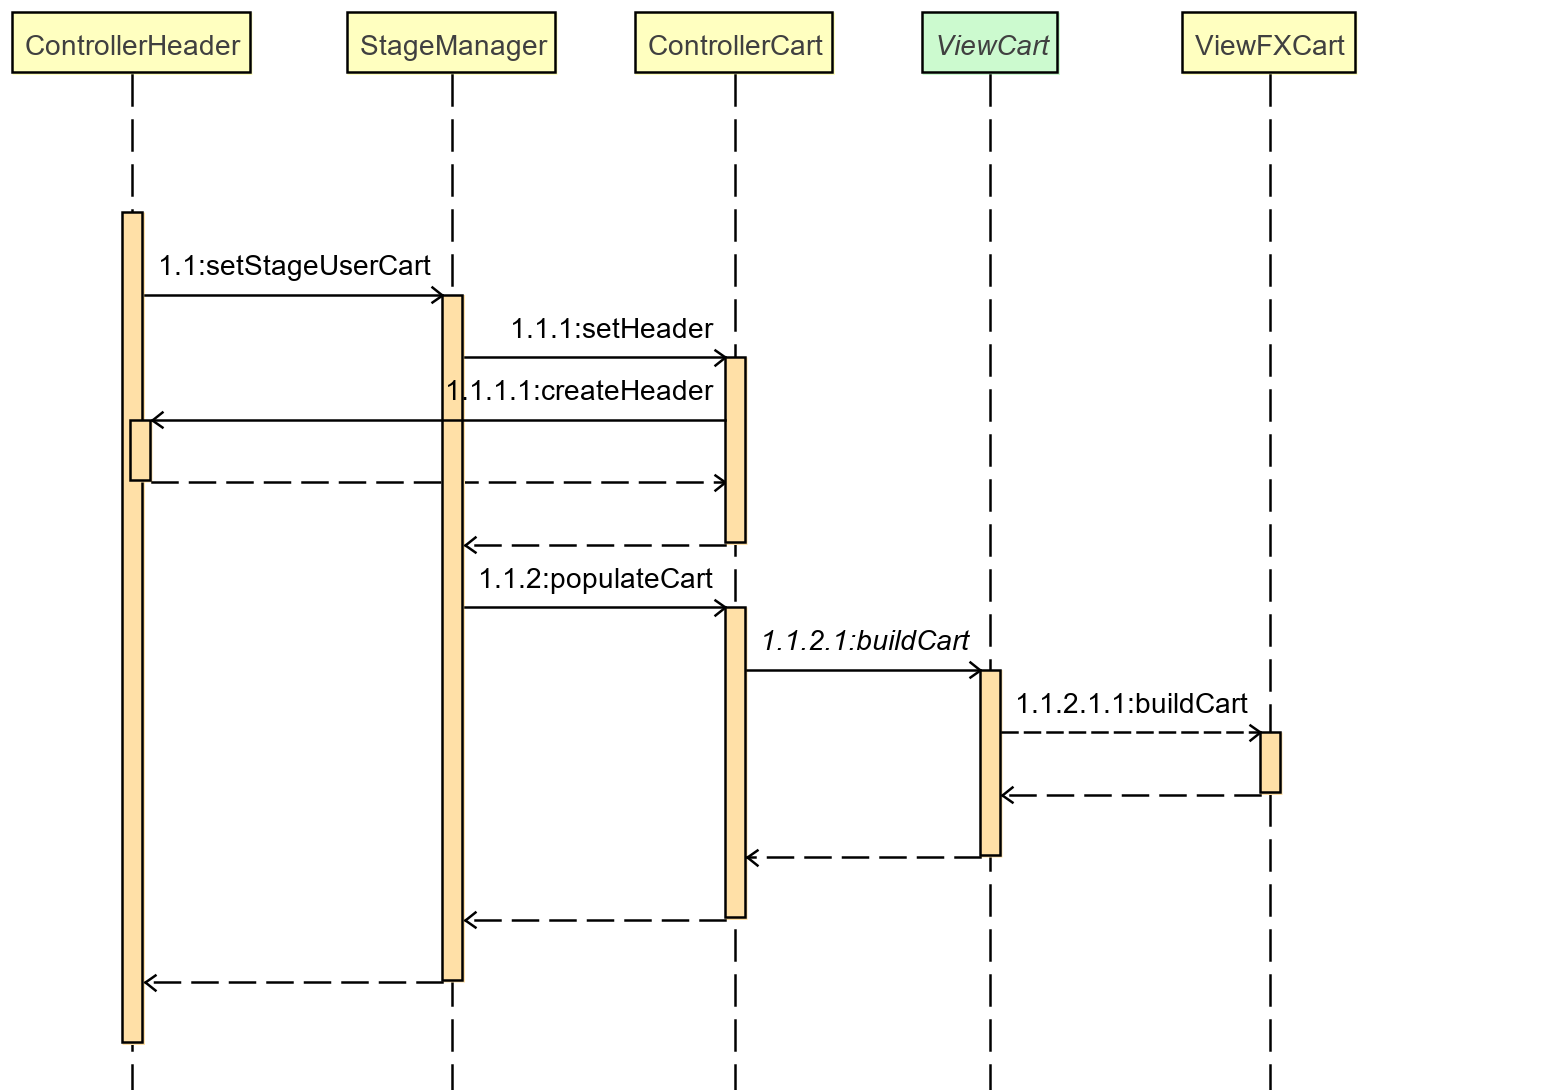
\includegraphics[width=1.2\linewidth]{Sequence diagrams/2 Order Creation/ViewCart senza metodi privati.png}
    	\caption{Diagramma sequenza visualizza carrello utente registrato - rato}
    	\label{visualizza carrello}
    \end{figure}\\

\clearpage
Dopo aver cliccato sul carrello l'utente ha la possibilità di modificare il carrello rimuovendo alcuni libri inseriti oppure può procedere al pagamento.\\
Se l'utente clicca su "Remove book from cart", la struttura dati utilizzata per il carrello, in questo caso una mappa, viene aggiornata e si ricostruisce la schermata, dunque il diagramma di sequenza è analogo a quello presentato sopra \ref{visualizza carrello}.\\
\newline
Presentiamo ora invece il diagramma delle sequenze di cosa succede se l'utente dalla schermata del carrello preme sul pulsante "Proceed to CheckOut":\\
\newline
    \begin{figure}[h!]
    	\centering
    	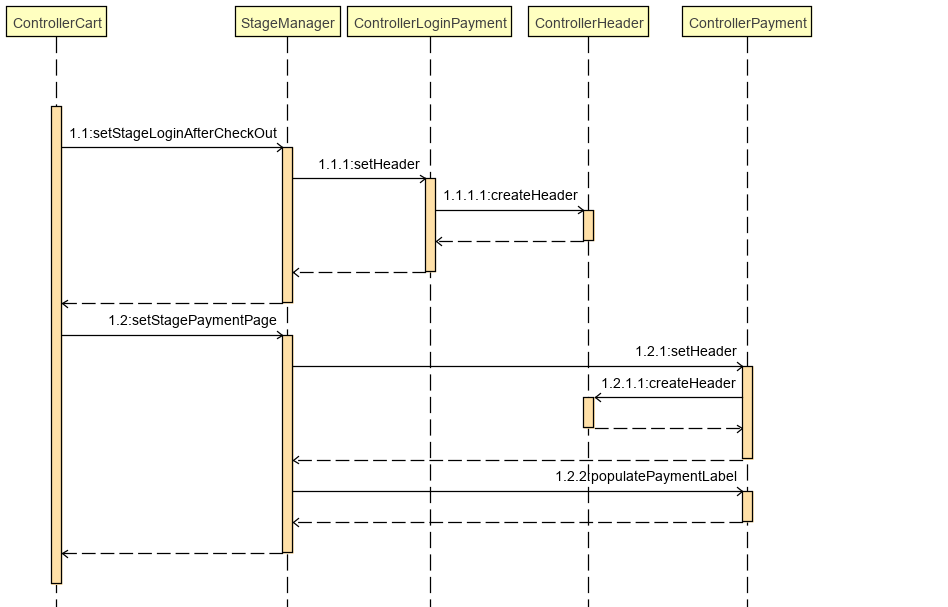
\includegraphics[width=1.1\linewidth]{Sequence diagrams/2 Order Creation/Proceed To checkout (tolte chiamate inutili a ViewHeader).png}
    	\caption{Diagramma sequenza pagamento utente registrato - utente non registrato}
    	\label{visualizza carrello}
    \end{figure}\\

Notiamo che la prima parte del diagramma di sequenza ovvero la chiamata al metodo "\textit{setStageLoginAfterCheckOut}" è inerente alla possibilità che l'utente registrato non si sia ancora autenticato oppure alla possibilità che l'utente sia non registrato.\\
\clearpage
Presentiamo quindi i diagrammi di sequenza per:
\begin{itemize}
    \item Autenticazione
    \item Registrazione
    \item Procedere senza registrazione
\end{itemize}
\leavevmode \newline
\begin{figure}[h!]
    	\centering
    	\hspace*{-0.4in}
    	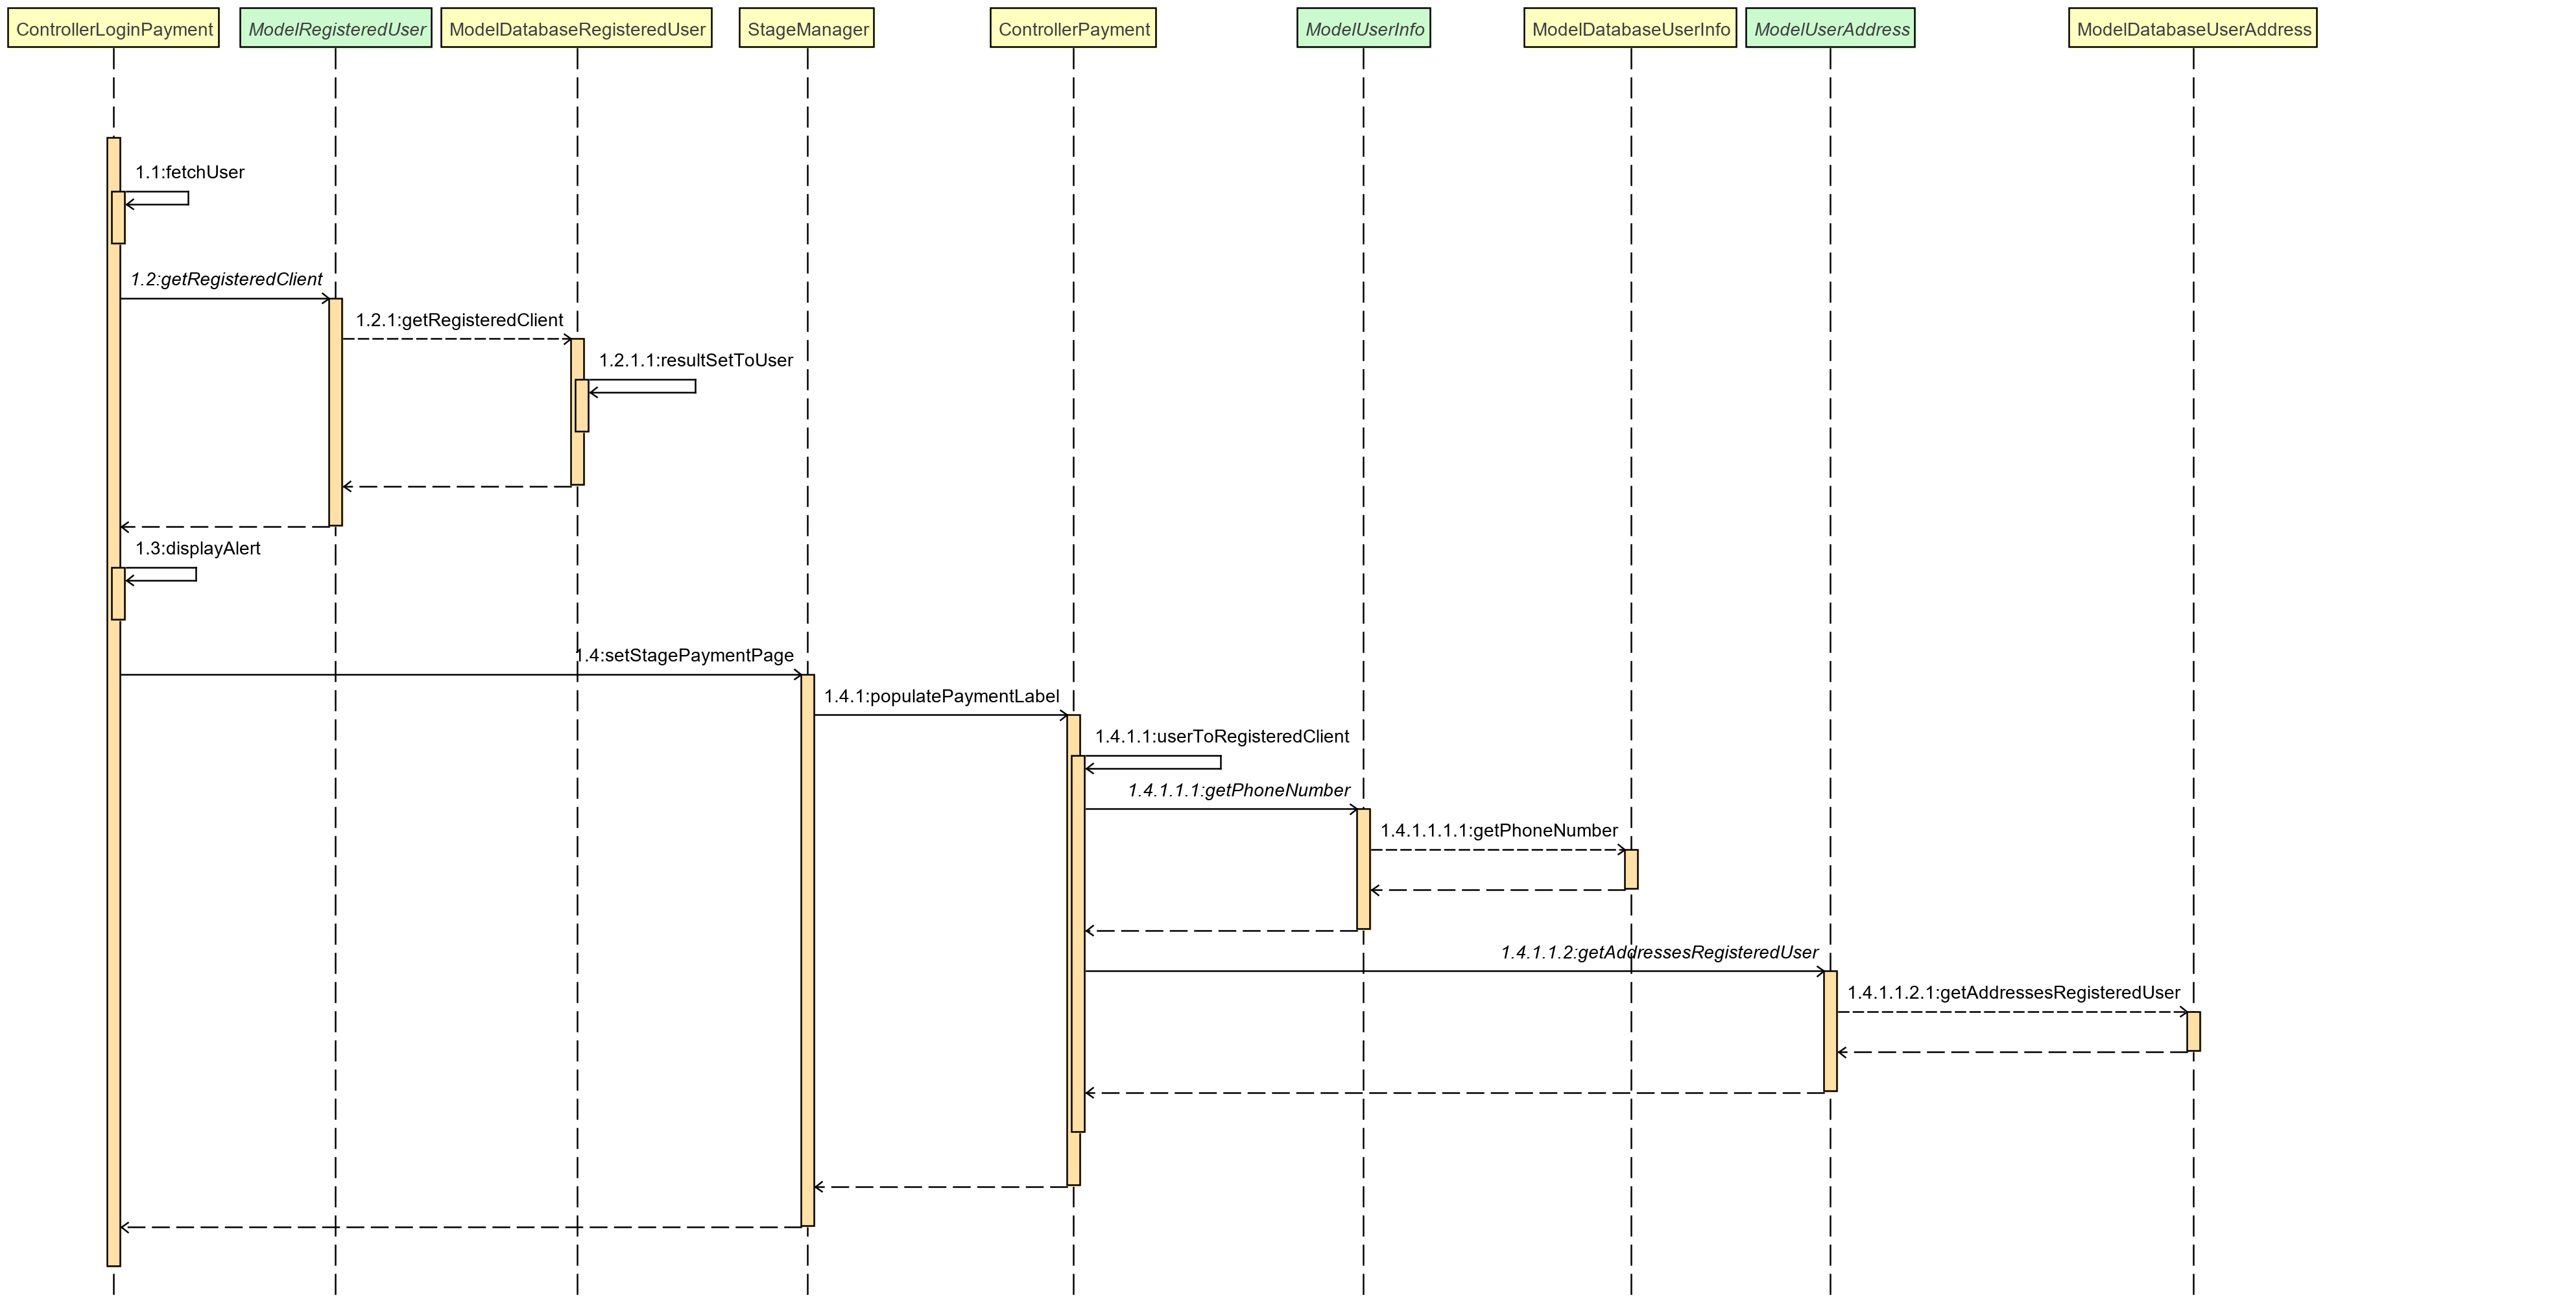
\includegraphics[width=1.1\linewidth]{Sequence diagrams/1 Registered user/regUser.png}
    	\caption{Diagramma sequenza autenticazione utente registrato}
    \end{figure} \leavevmode \\
    
In questo diagramma sequenza e nei successivi abbiamo inserito qualche dettaglio in più rispetto ai precedenti al fine di mostrare l'utilizzo del Database per la gestione delle varie tipologie di utenti.\\

\leavevmode \newline
La struttura e l'utilizzo del database nel dettaglio vengono presentati, come detto in precedenza, al capitolo inerente alle scelte progettuali e allo sviluppo del sistema.

\clearpage
\begin{figure}[h!]
    	\centering
    	\hspace*{-0.4in}
    	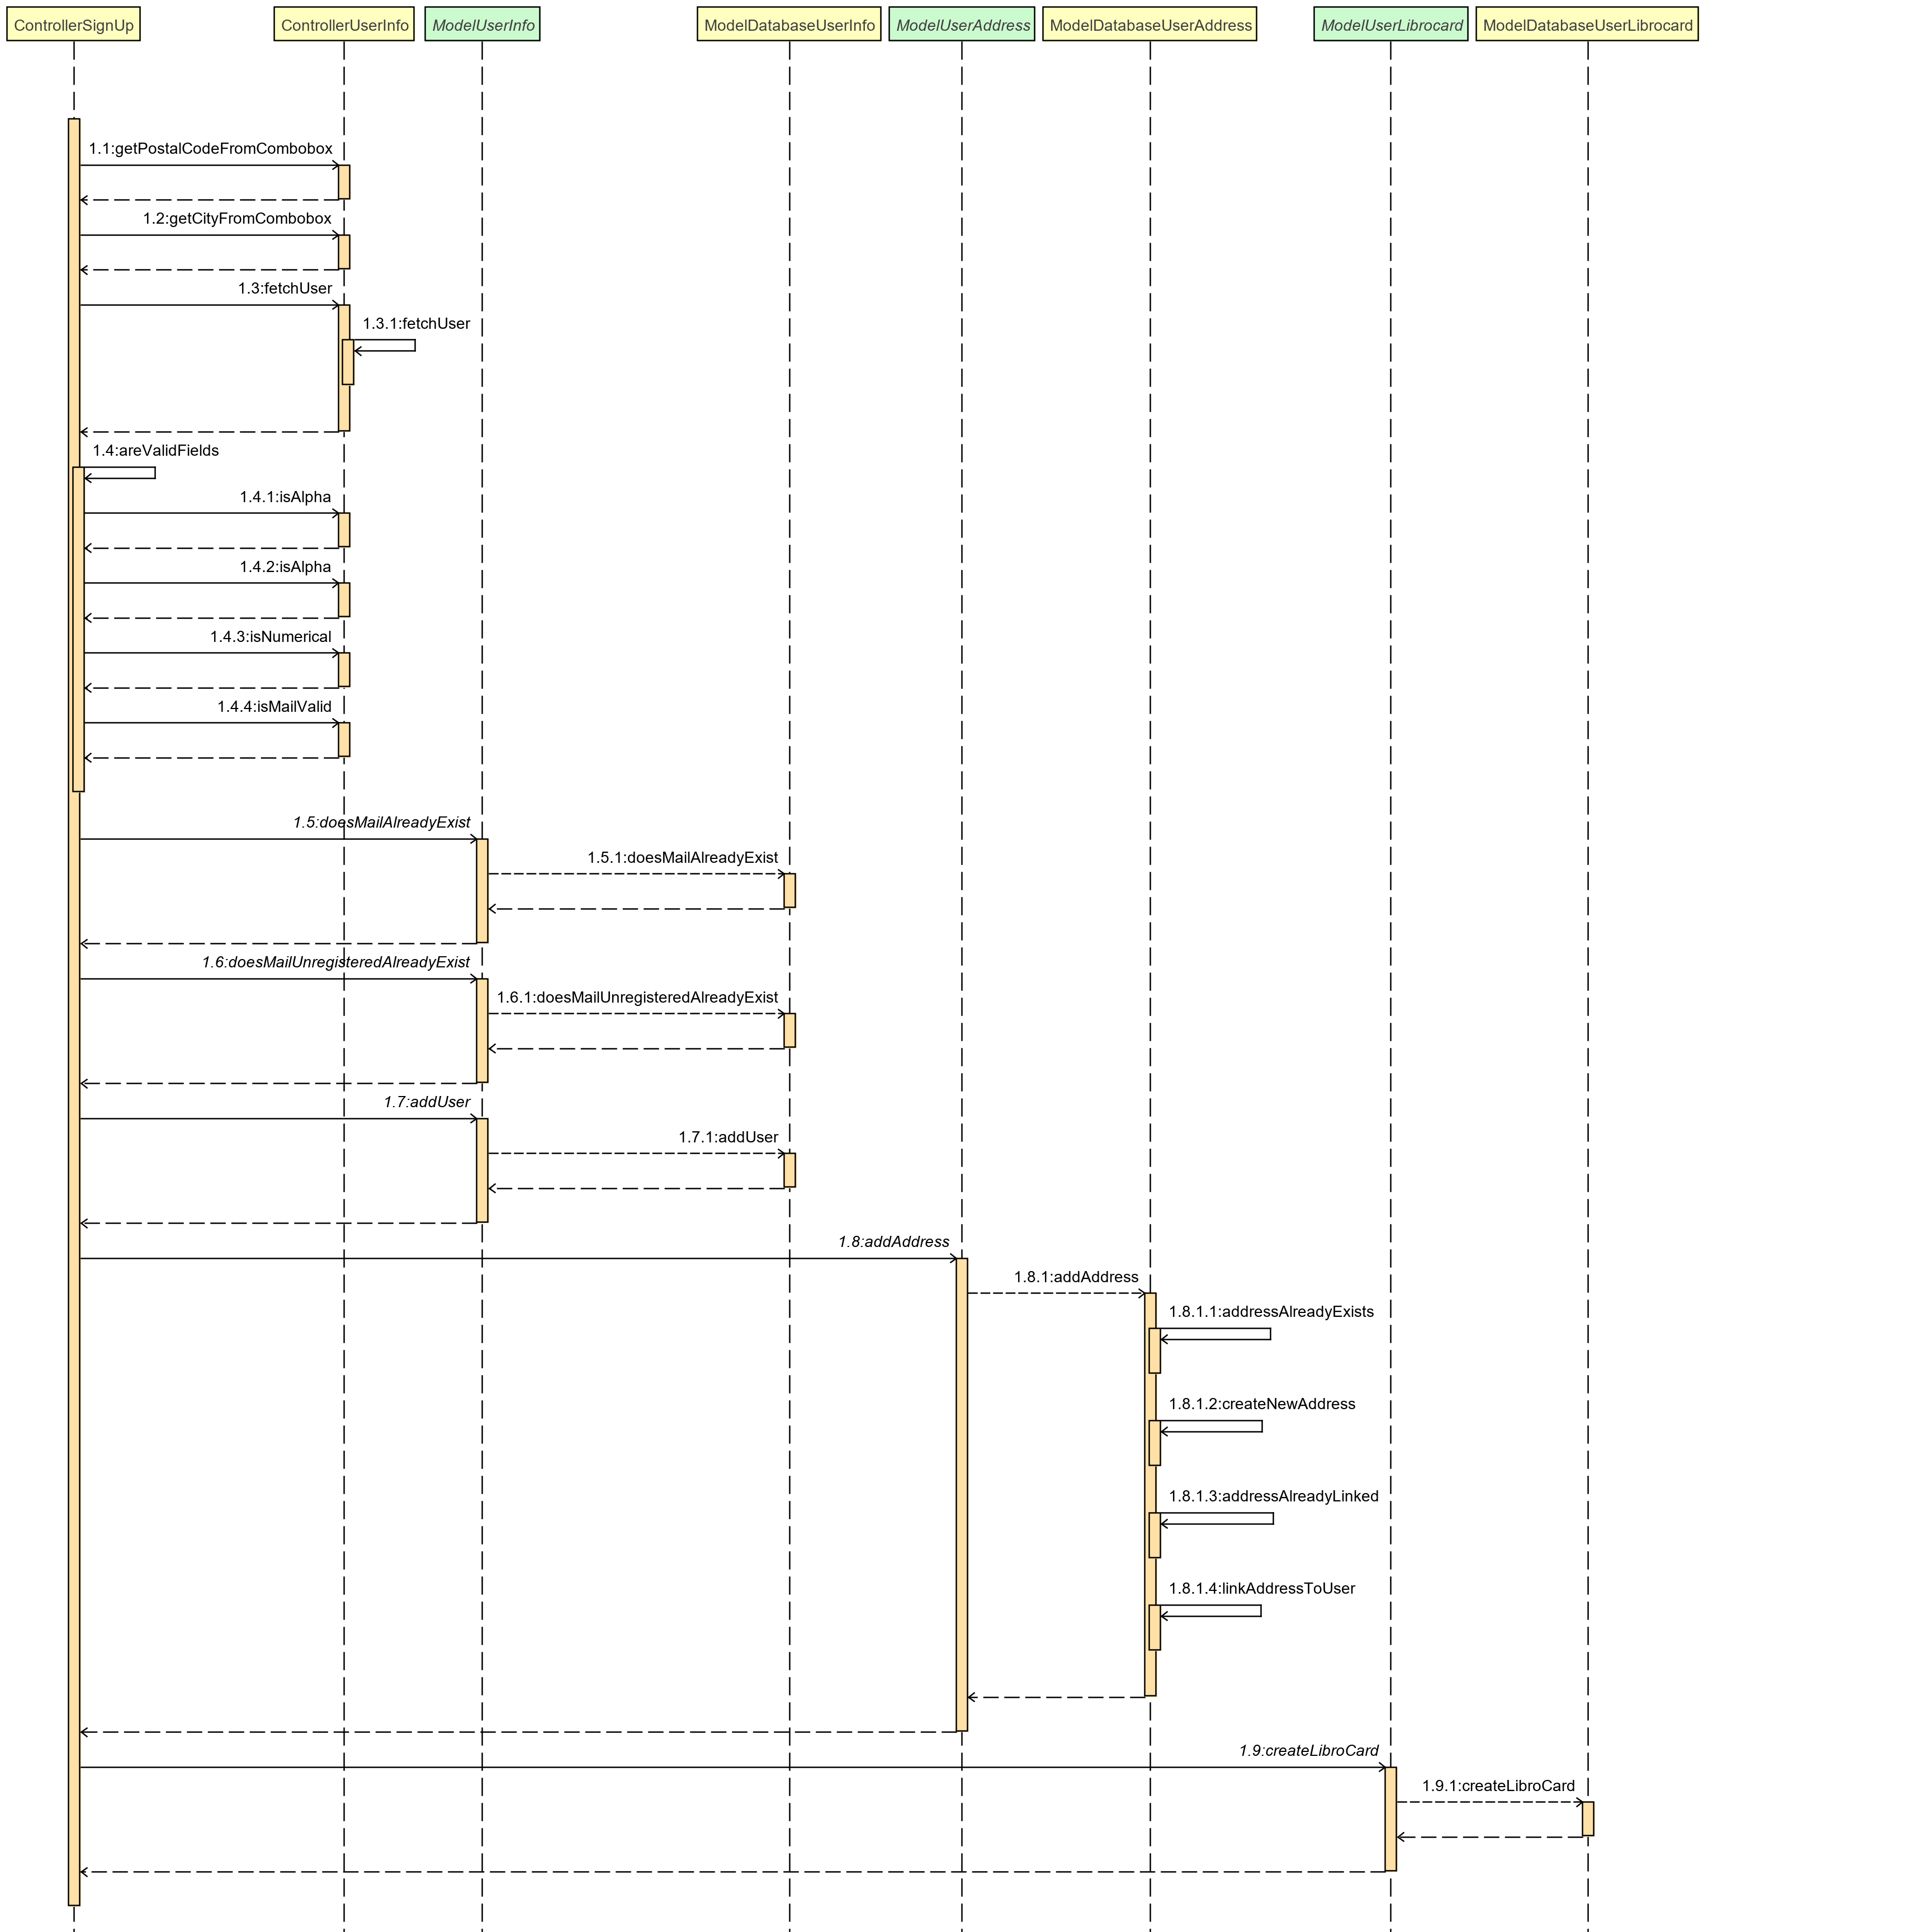
\includegraphics[width=1.3\linewidth]{Sequence diagrams/1 Registered user/signUp.png}
    	\caption{Diagramma sequenza registrazione utente non registrato}
    \end{figure}

Per la registrazione di un utente si recuperano tutte le informazioni, successivamente si verifica nel DB che la mail sia univoca. A questo punto, se i dati inseriti sono corretti, si aggiunge l'utente e si collega all'indirizzo di spedizione scelto.
\clearpage
\begin{figure}[h!]
    	\centering
    	\hspace*{-0.4in}
    	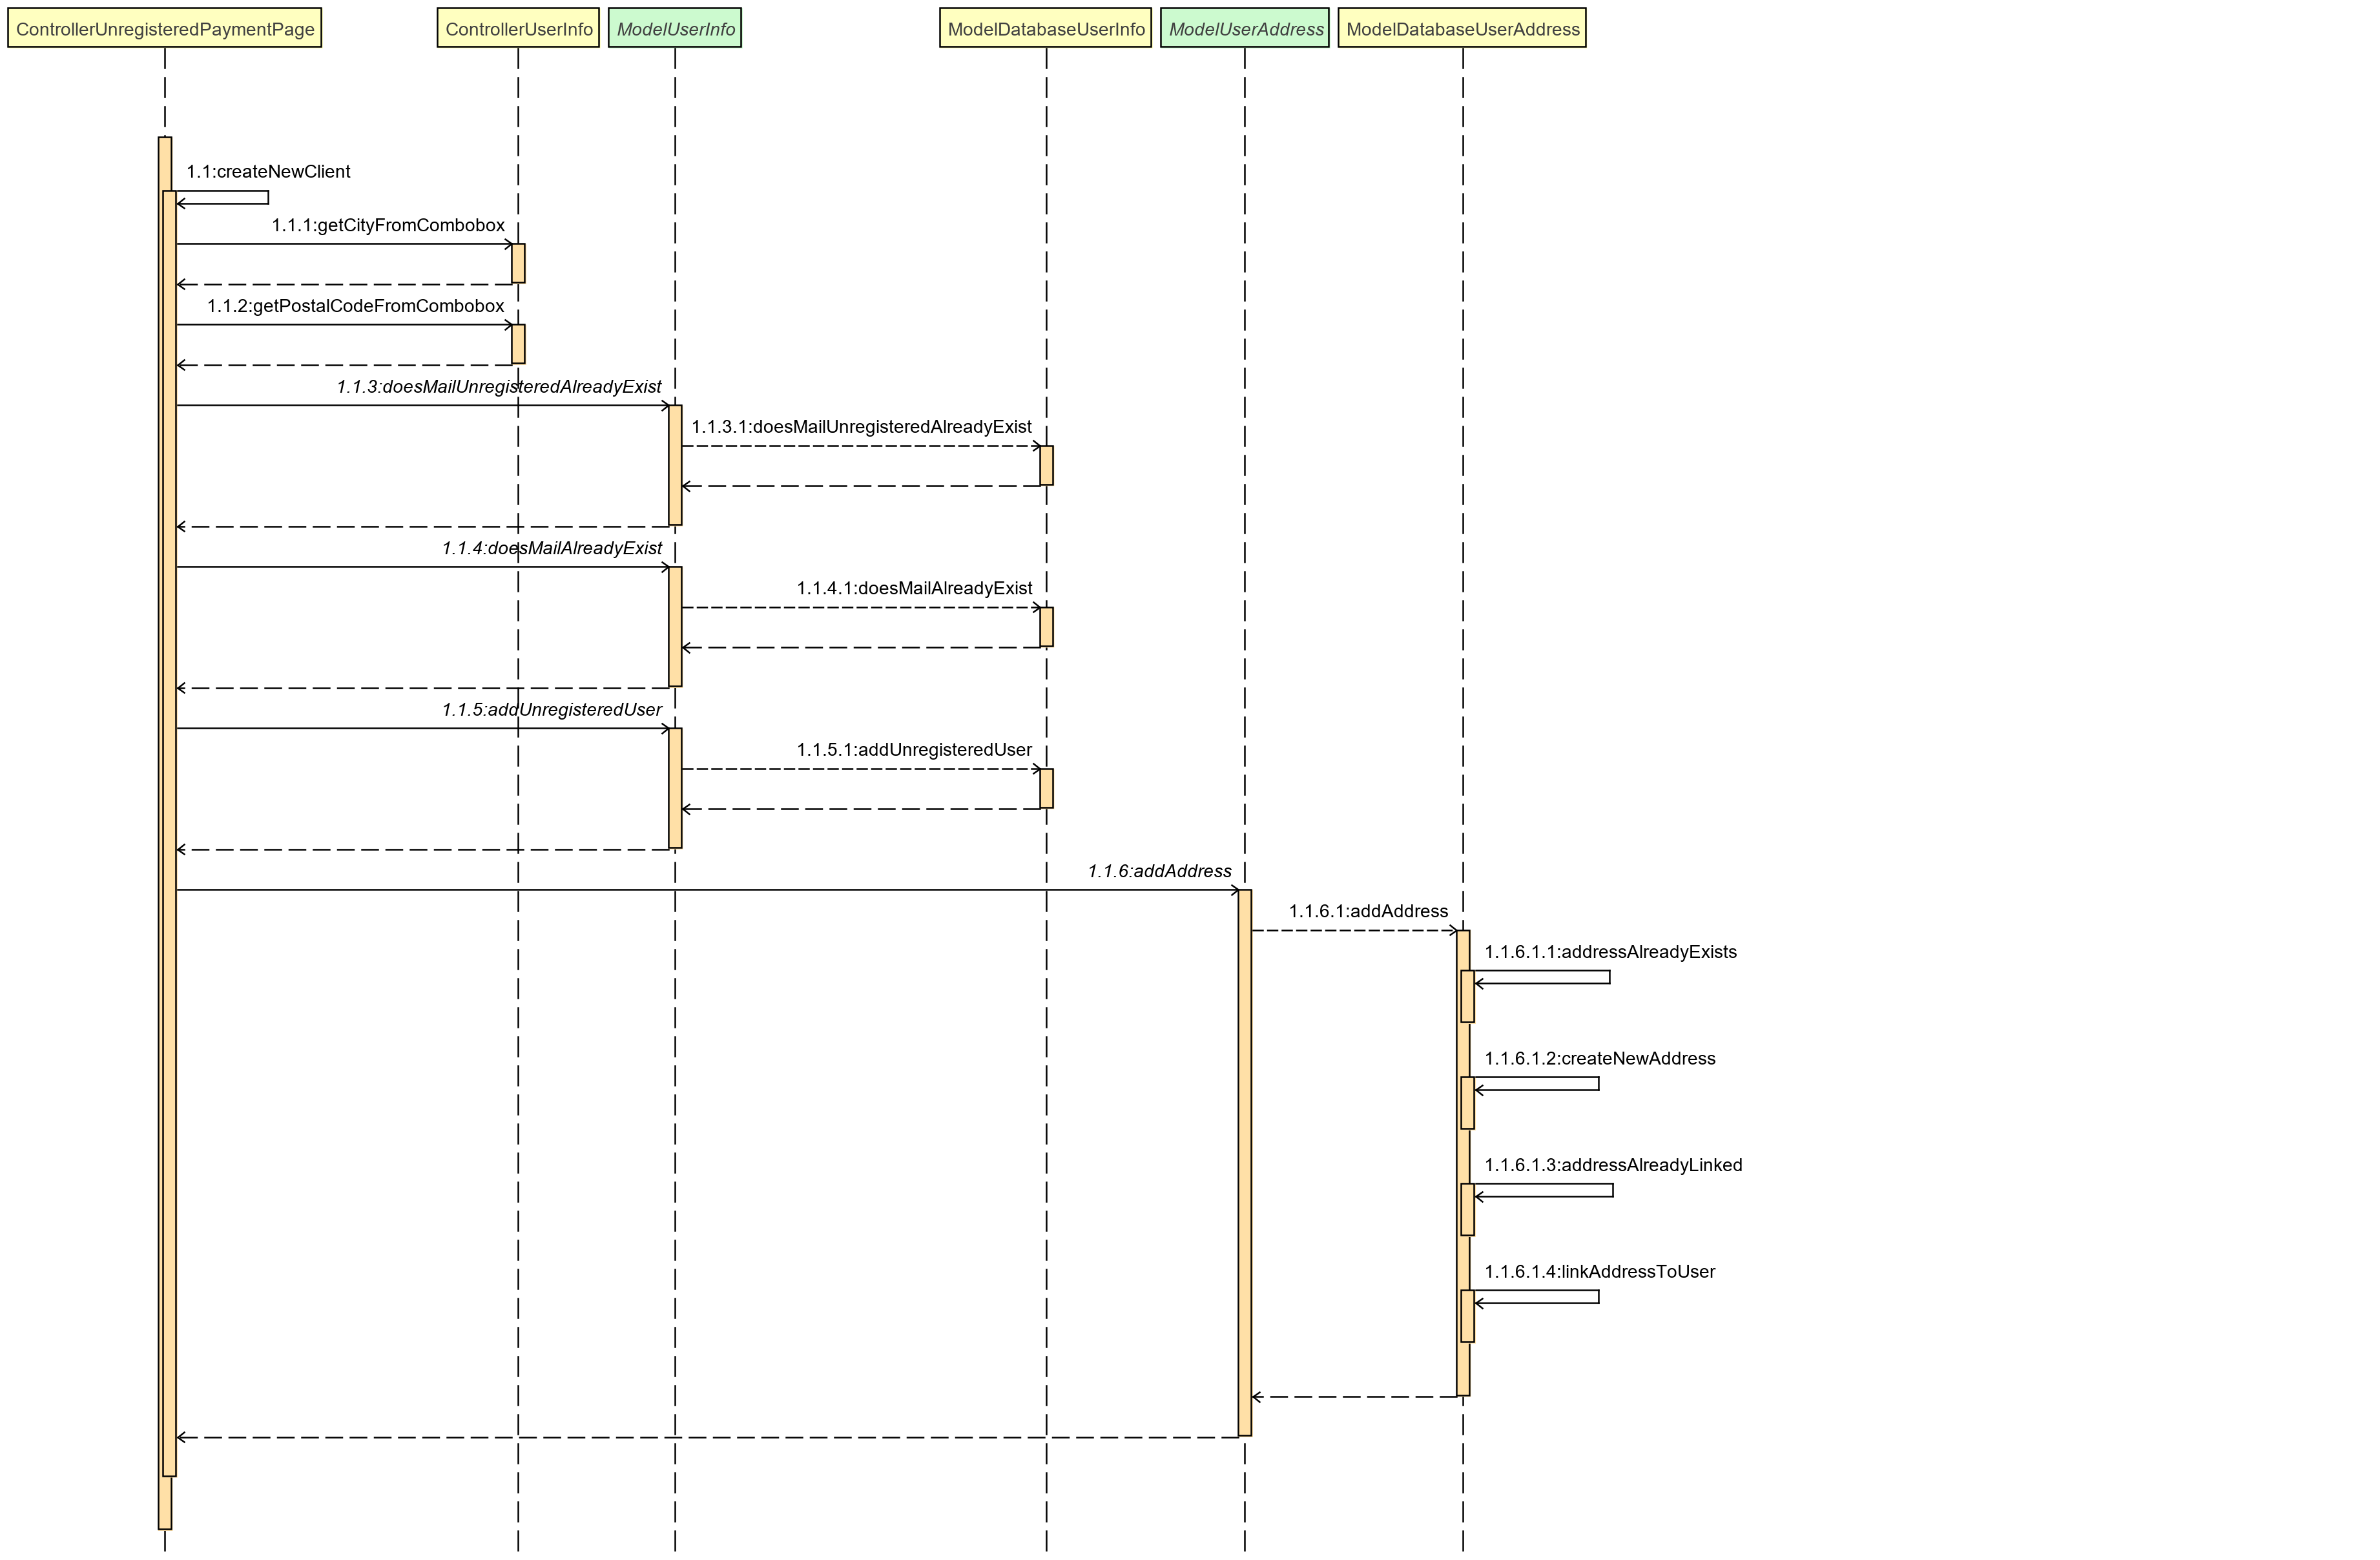
\includegraphics[width=1.3\linewidth]{Sequence diagrams/2 Order Creation/continueAsUnreg.png}
    	\caption{Diagramma sequenza utente continua come non registrato}
    \end{figure} \leavevmode \\
\leavevmode \newline
Se l'utente decide di proseguire alla creazione dell'ordine senza registrarsi, il sistema comunque gli richiede tutte le informazioni al fine di poterlo identificare come utente non registrato.\\
Quindi vengono richiesti i sui dati anagrafici, una mail che deve essere univoca e un indirizzo di spedizione: se i dati forniti sono validi l'utente viene aggiunto al DB (come non registrato) e condotto alla pagina di pagamento.\\
\clearpage

Viene qui di seguito riportato il diagramma delle sequenze \underline{dell'utente responsabile} per \textbf{visualizzare ordini} e \textbf{aggiornare lo stato dell'ordine}:\\
\begin{figure}[h!]
    	\centering
    	\hspace*{-0.4in}
    	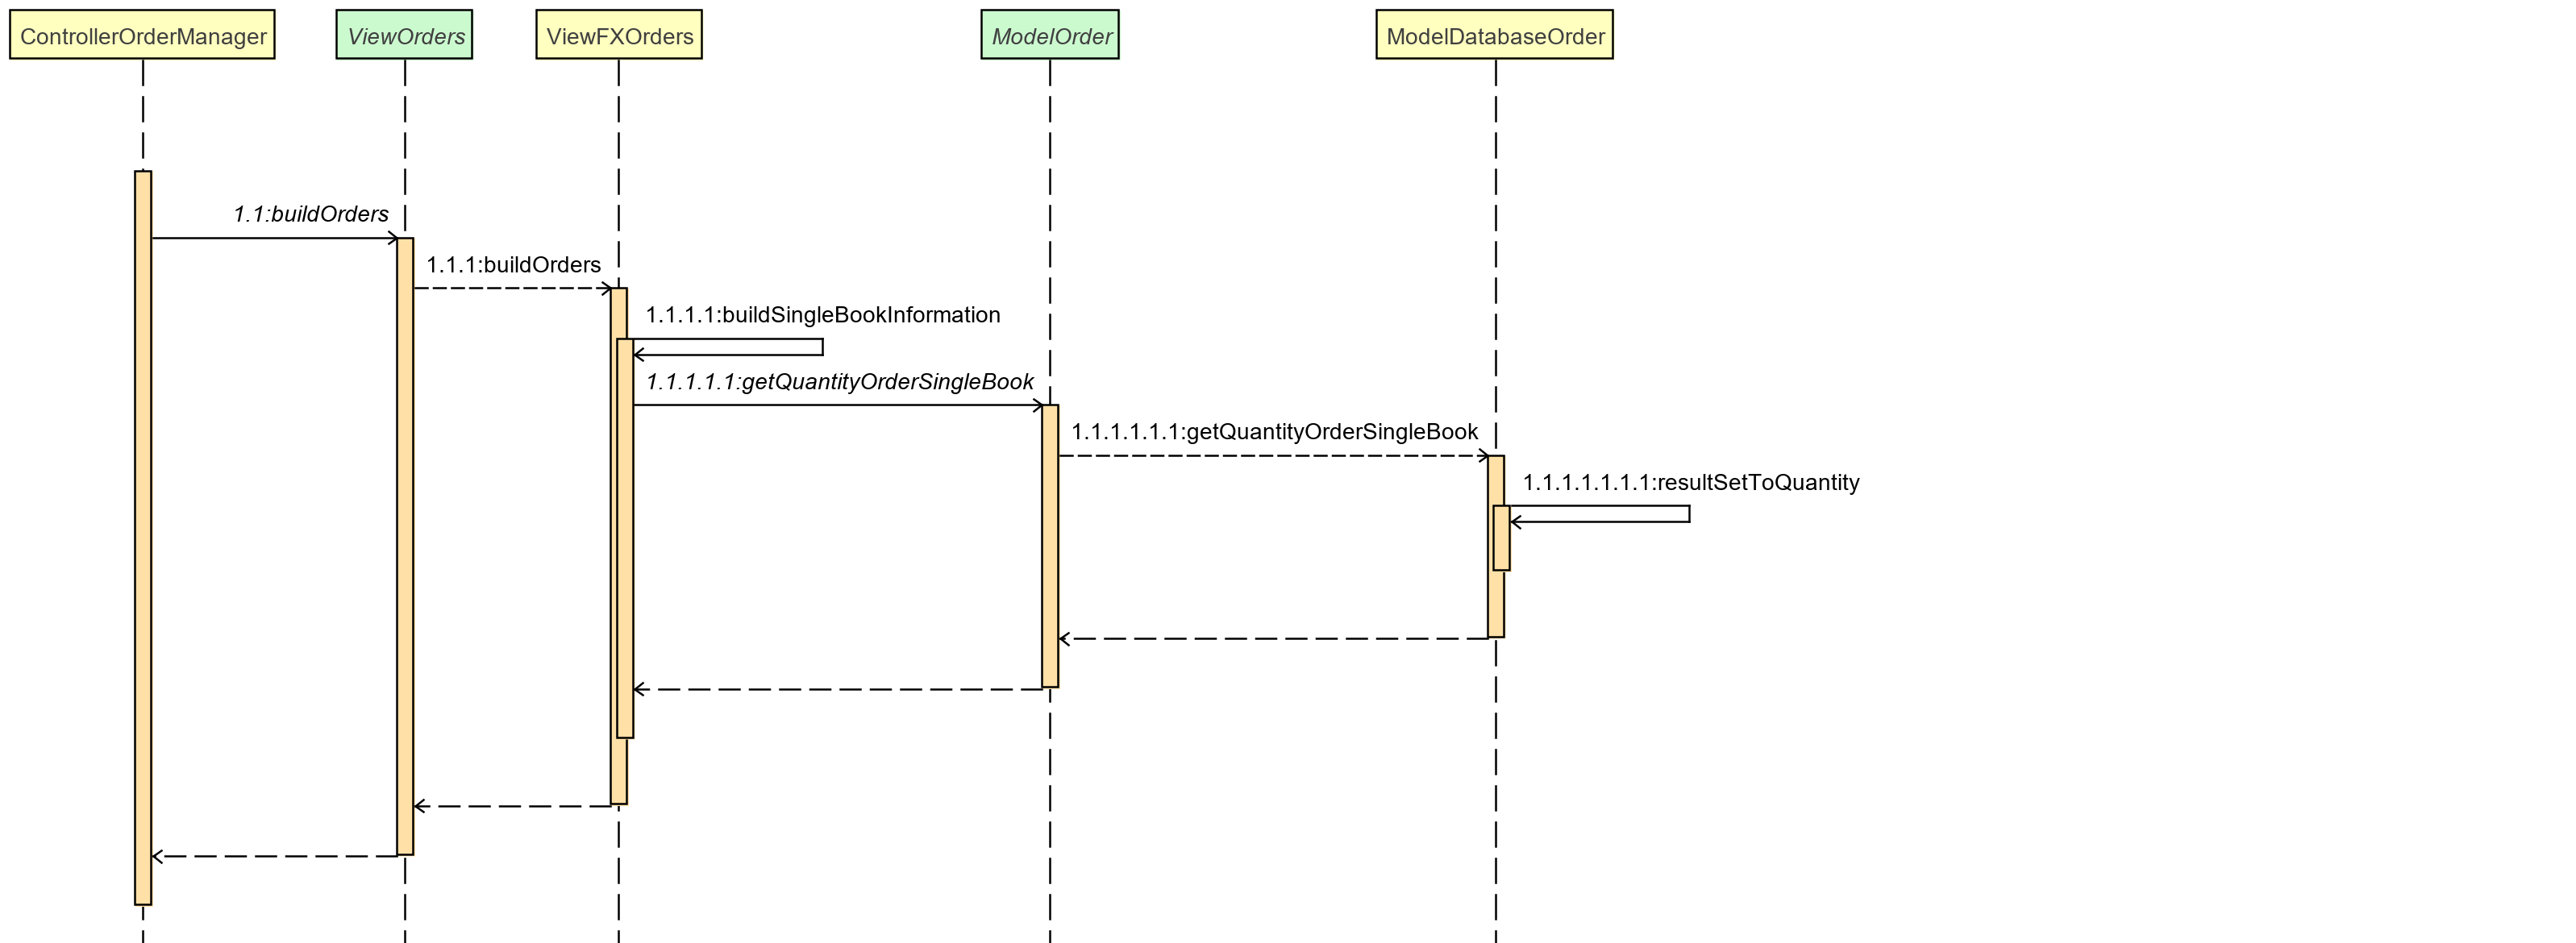
\includegraphics[width=1.7\linewidth]{Sequence diagrams/3 Manager/viewOrderManager.png}
    	\caption{Diagramma sequenza utente responsabile visualizza ordine utenti}
    \end{figure}\\
    
    \begin{figure}[h!]
    	\centering
    	\hspace*{-0.4in}
    	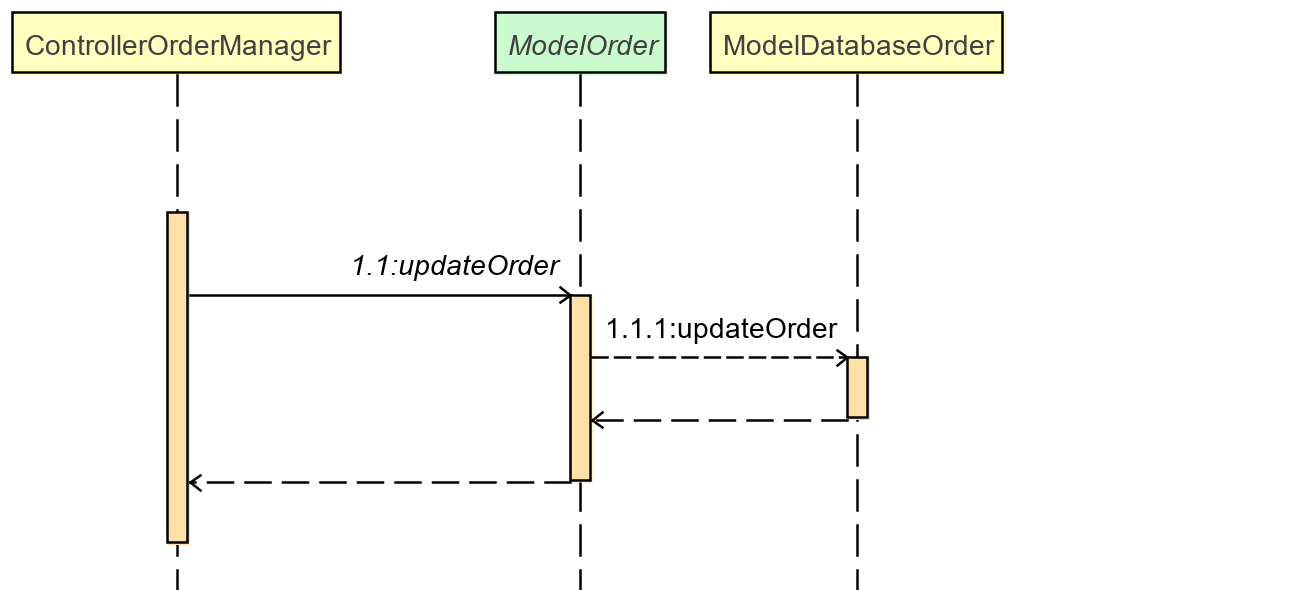
\includegraphics[width=1.0\linewidth]{Sequence diagrams/3 Manager/updateOrderStatus.png}
    	\caption{Diagramma sequenza utente responsabile aggiorna stato ordine utenti}
    \end{figure}
\clearpage
Viene di seguito riportato il diagramma delle sequenze  \underline{dell'utente responsabile} per \textbf{aggiunta di un nuovo libro al catalogo} e \textbf{aggiornamento libro esistente}:\\
 \begin{figure}[h!]
    	\centering
    	\hspace*{-0.4in}
    	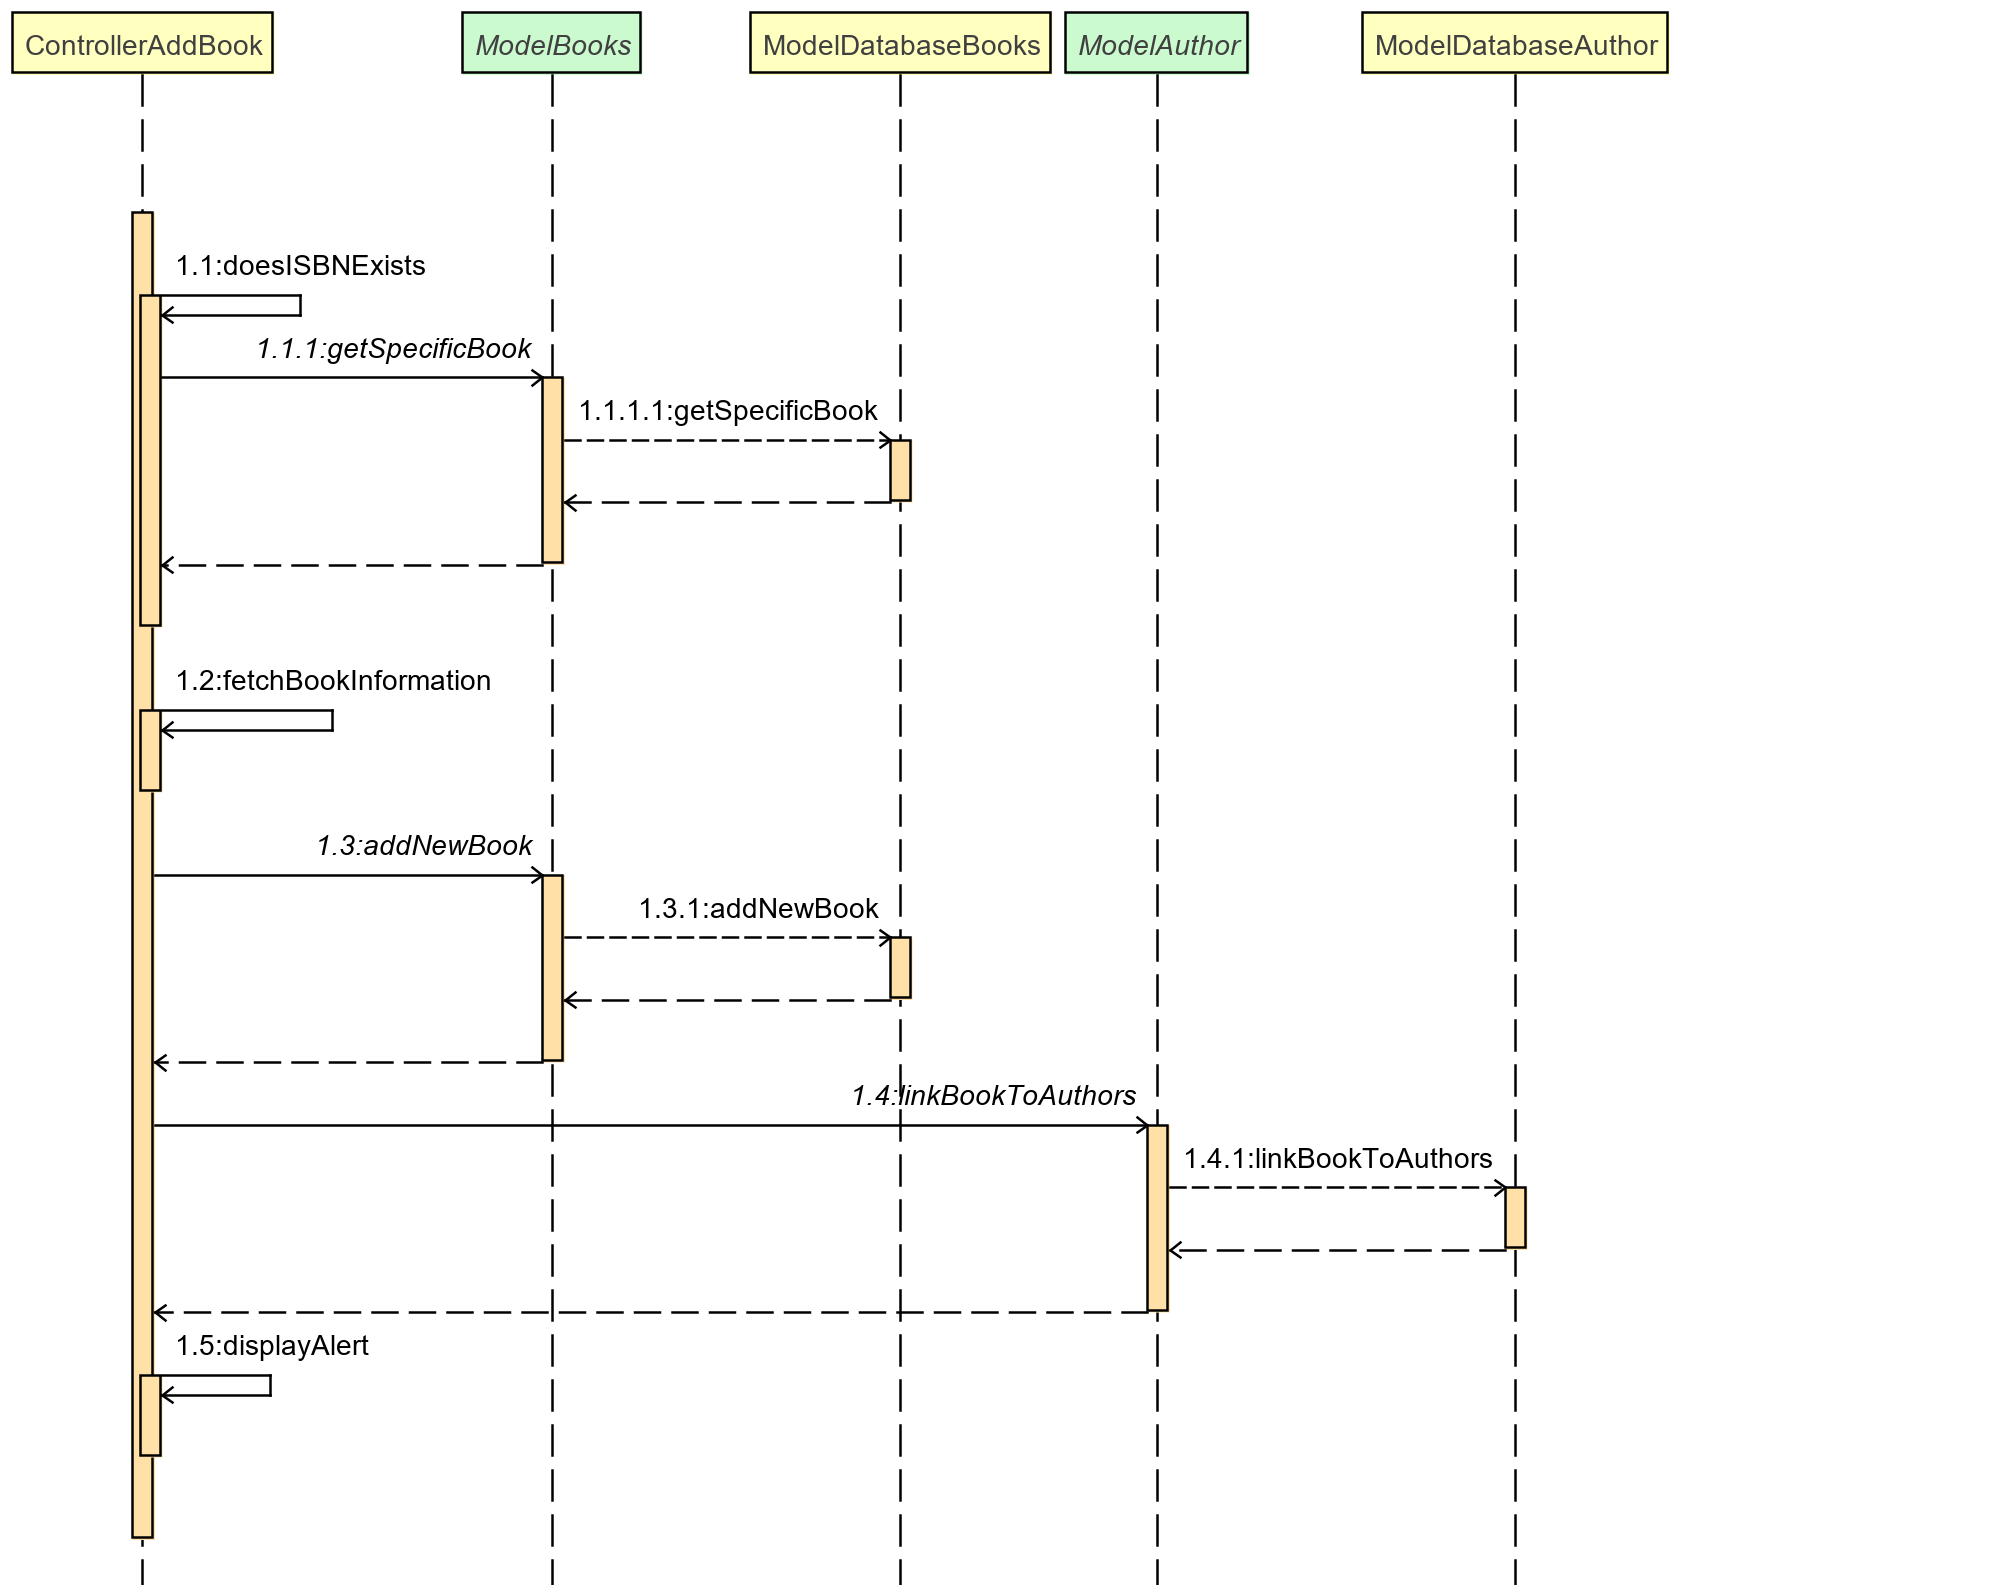
\includegraphics[width=1.4\linewidth]{Sequence diagrams/3 Manager/addBookToCatalogManager.png}
    	\caption{Diagramma sequenza utente responsabile aggiunta nuovo libro al catalogo}
    \end{figure}\\


\begin{figure}[h!]
    	\centering
    	\hspace*{-0.2in}
    	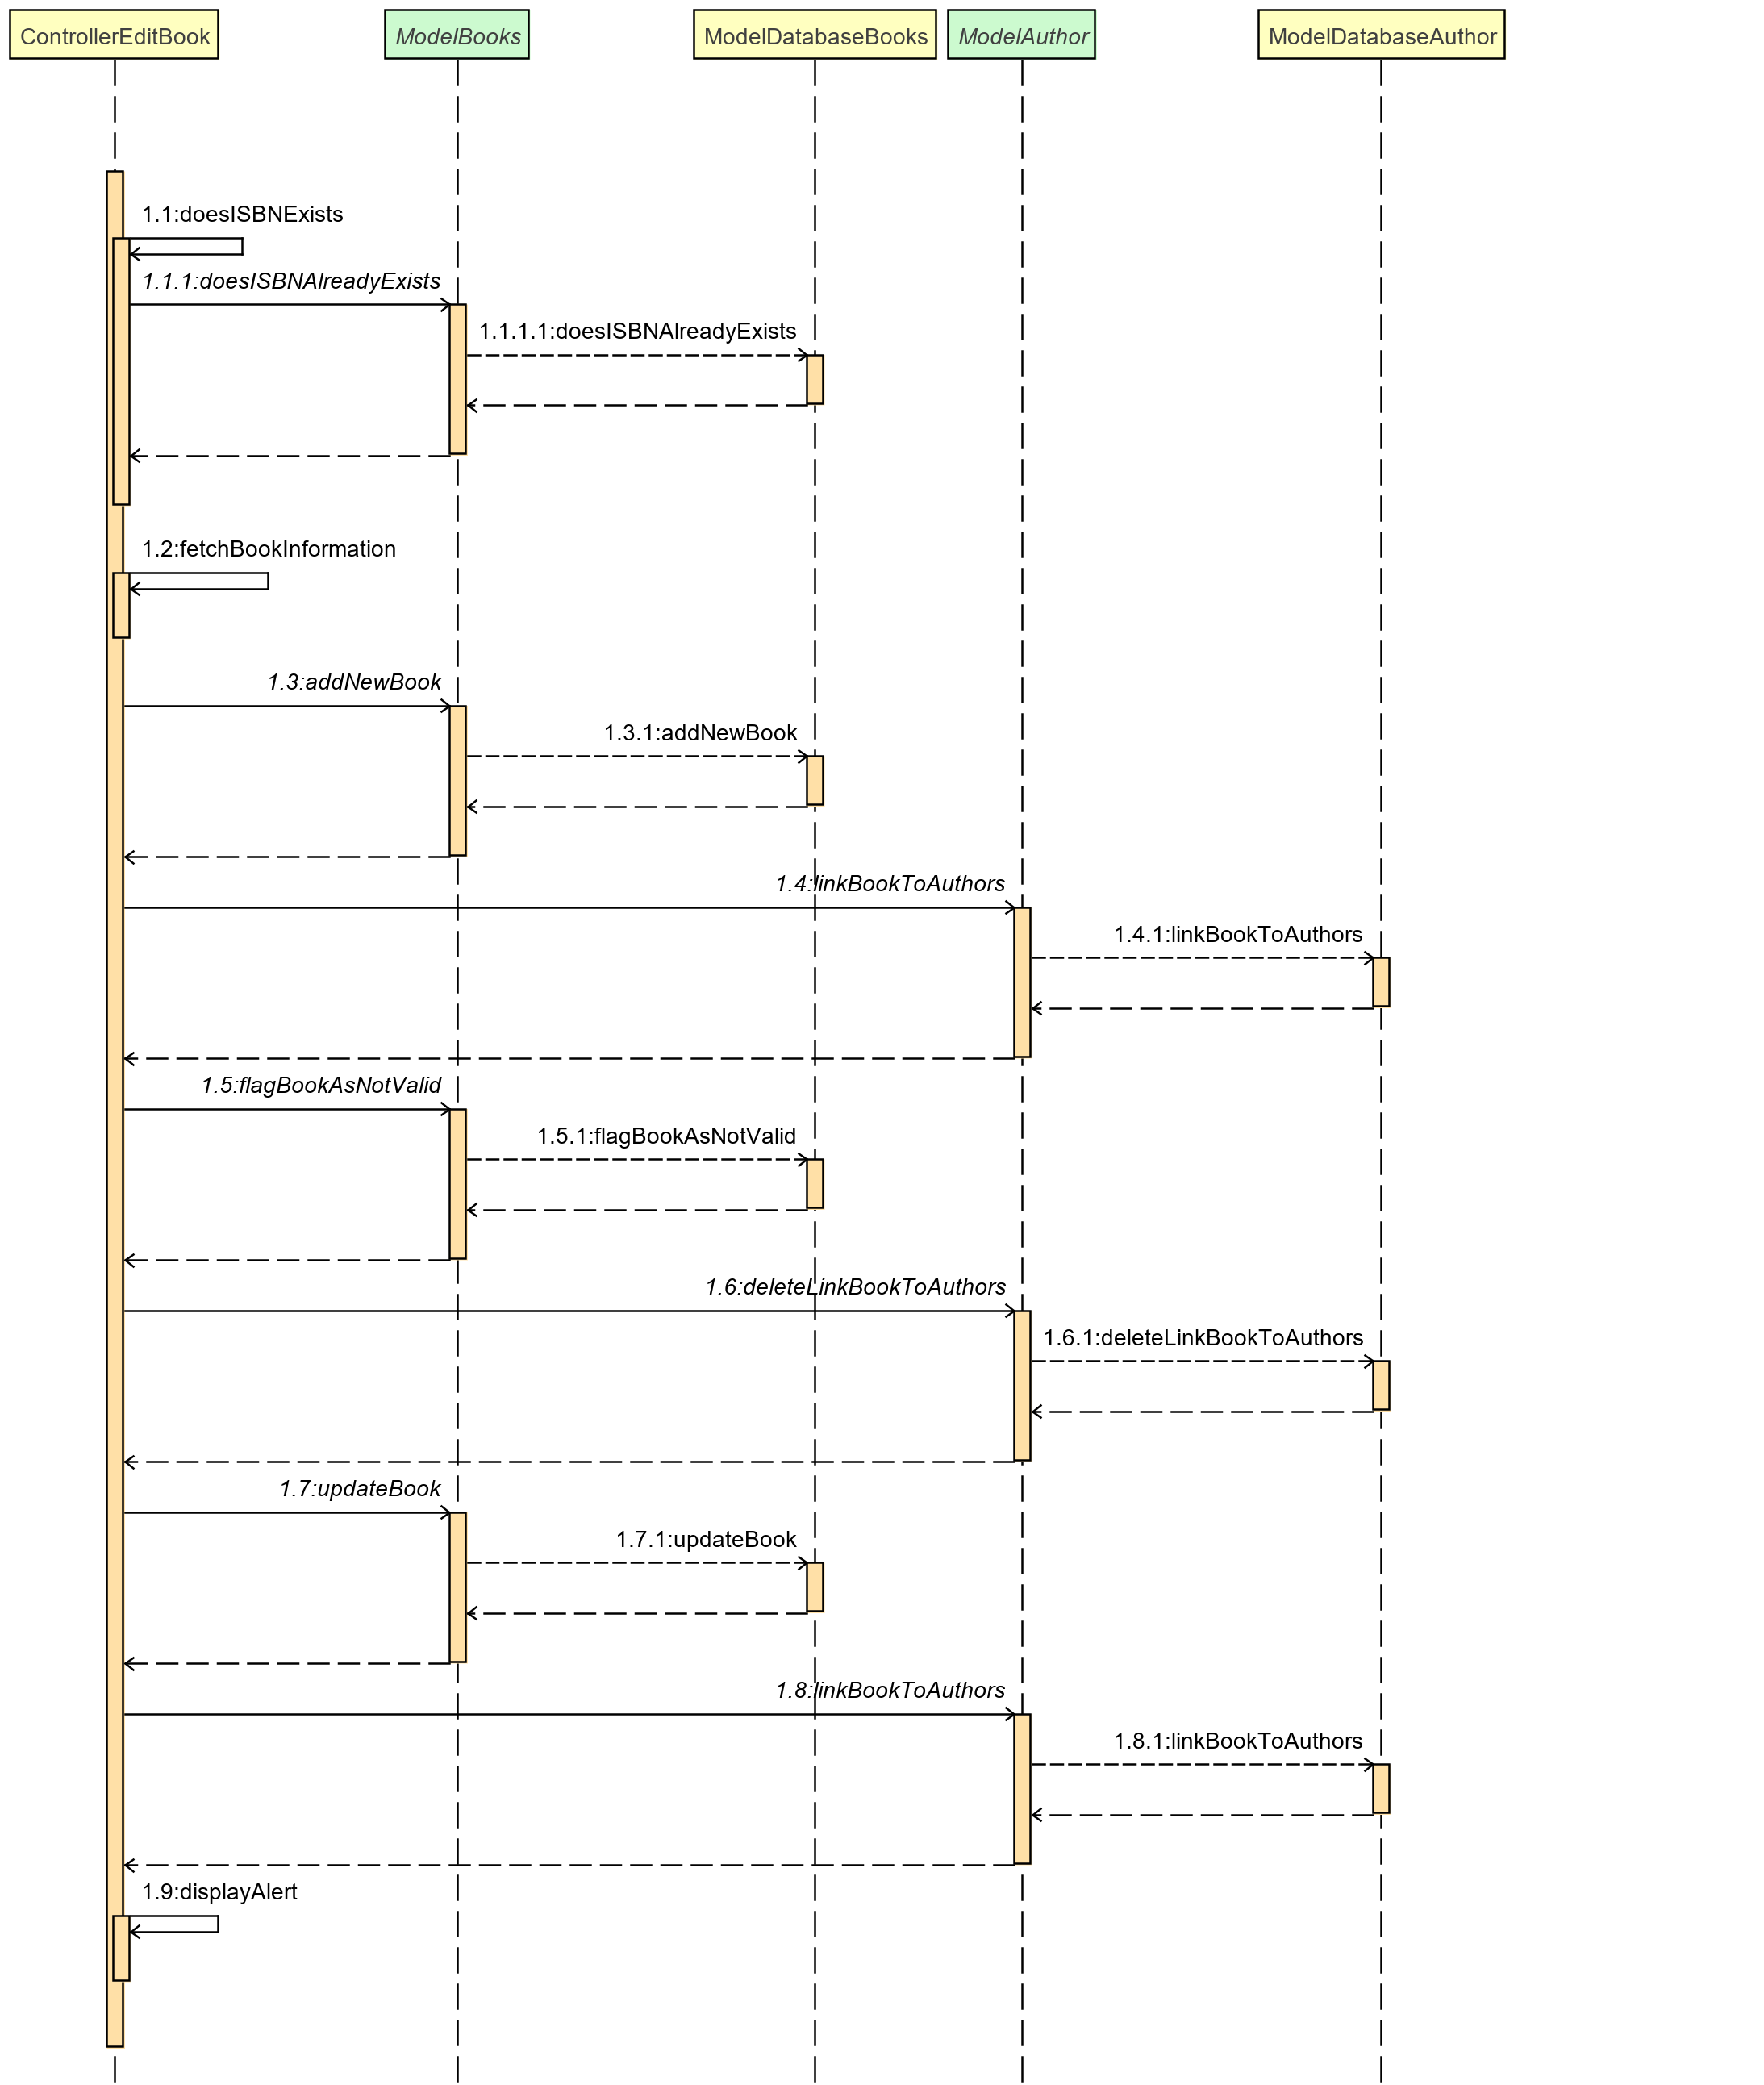
\includegraphics[width=1.3\linewidth]{Sequence diagrams/3 Manager/editBookManager.png}
    	\caption{Diagramma sequenza utente responsabile aggiorna informazioni libro esistente}
    \end{figure} \leavevmode \\
    
\clearpage
\begin{figure}[h!]
    	\centering
    	\hspace*{-0.2in}
    	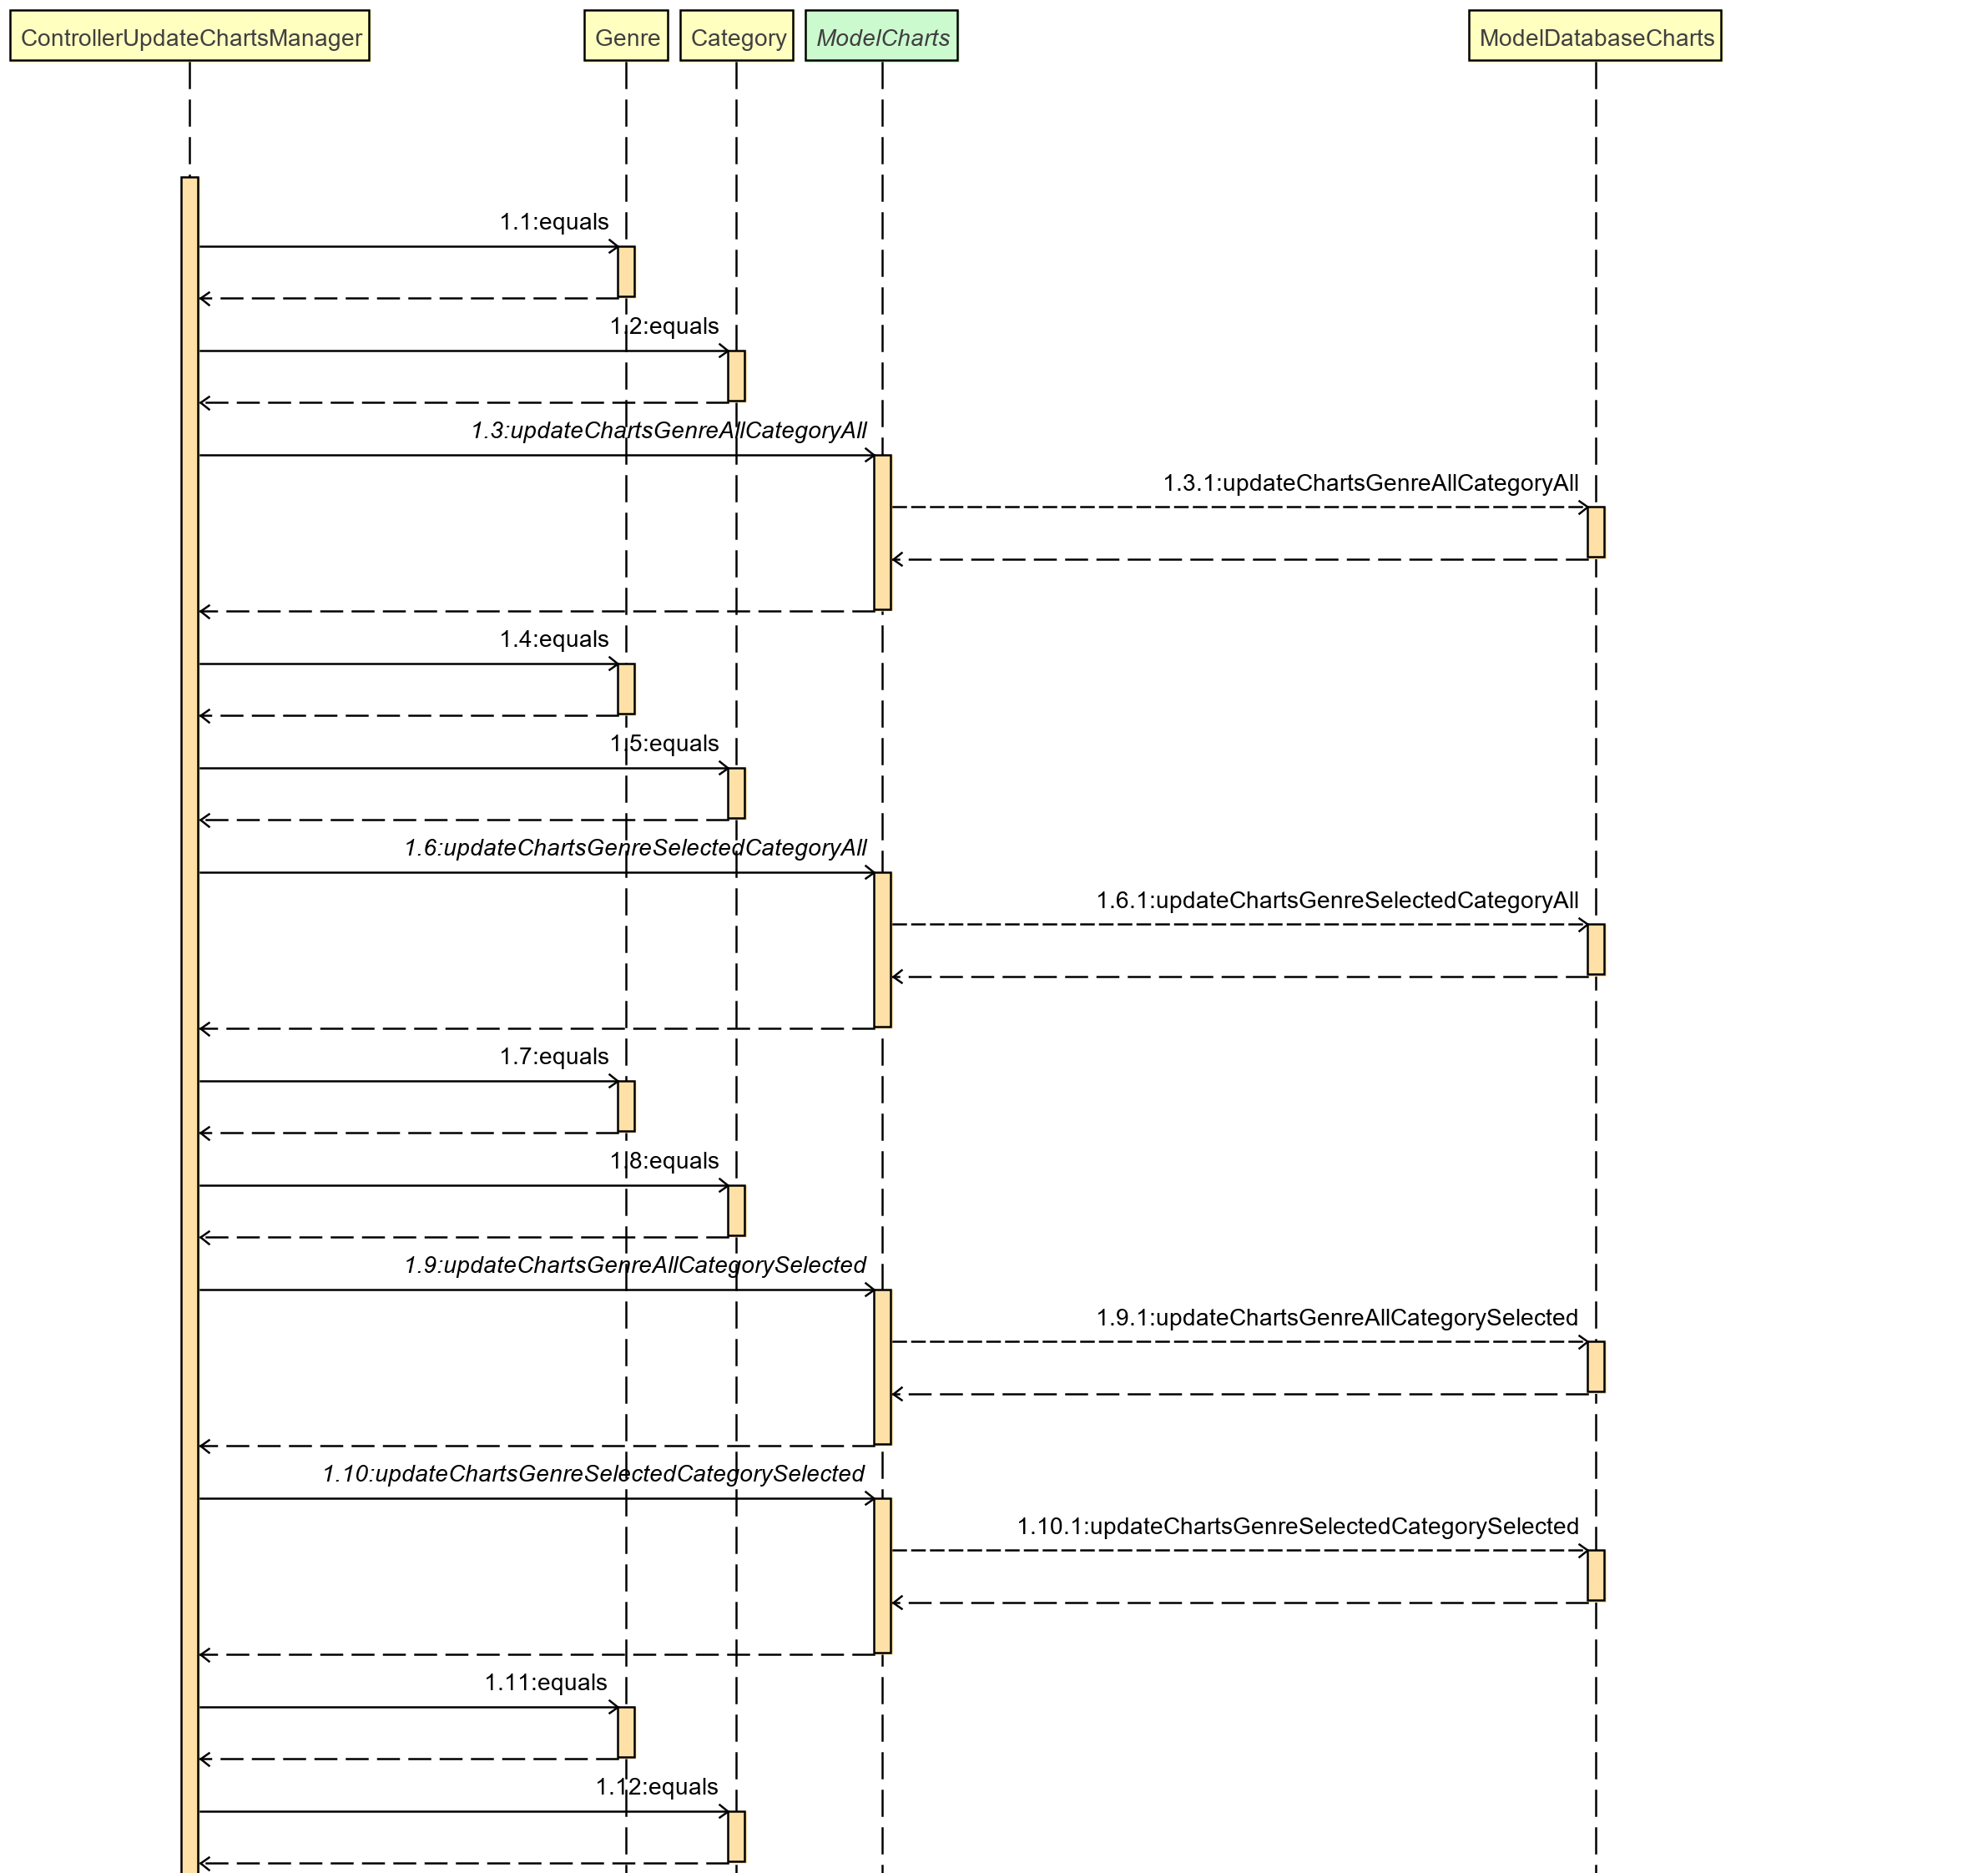
\includegraphics[width=1.3\linewidth]{Sequence diagrams/3 Manager/updateChartsManager.png}
    	\caption{Diagramma sequenza utente responsabile aggiorna classifiche libro}
    \end{figure}
    
    Continua nella seguente pagina
    \clearpage
\begin{figure}[h!]
	\centering
    	\hspace*{+0.3in}
	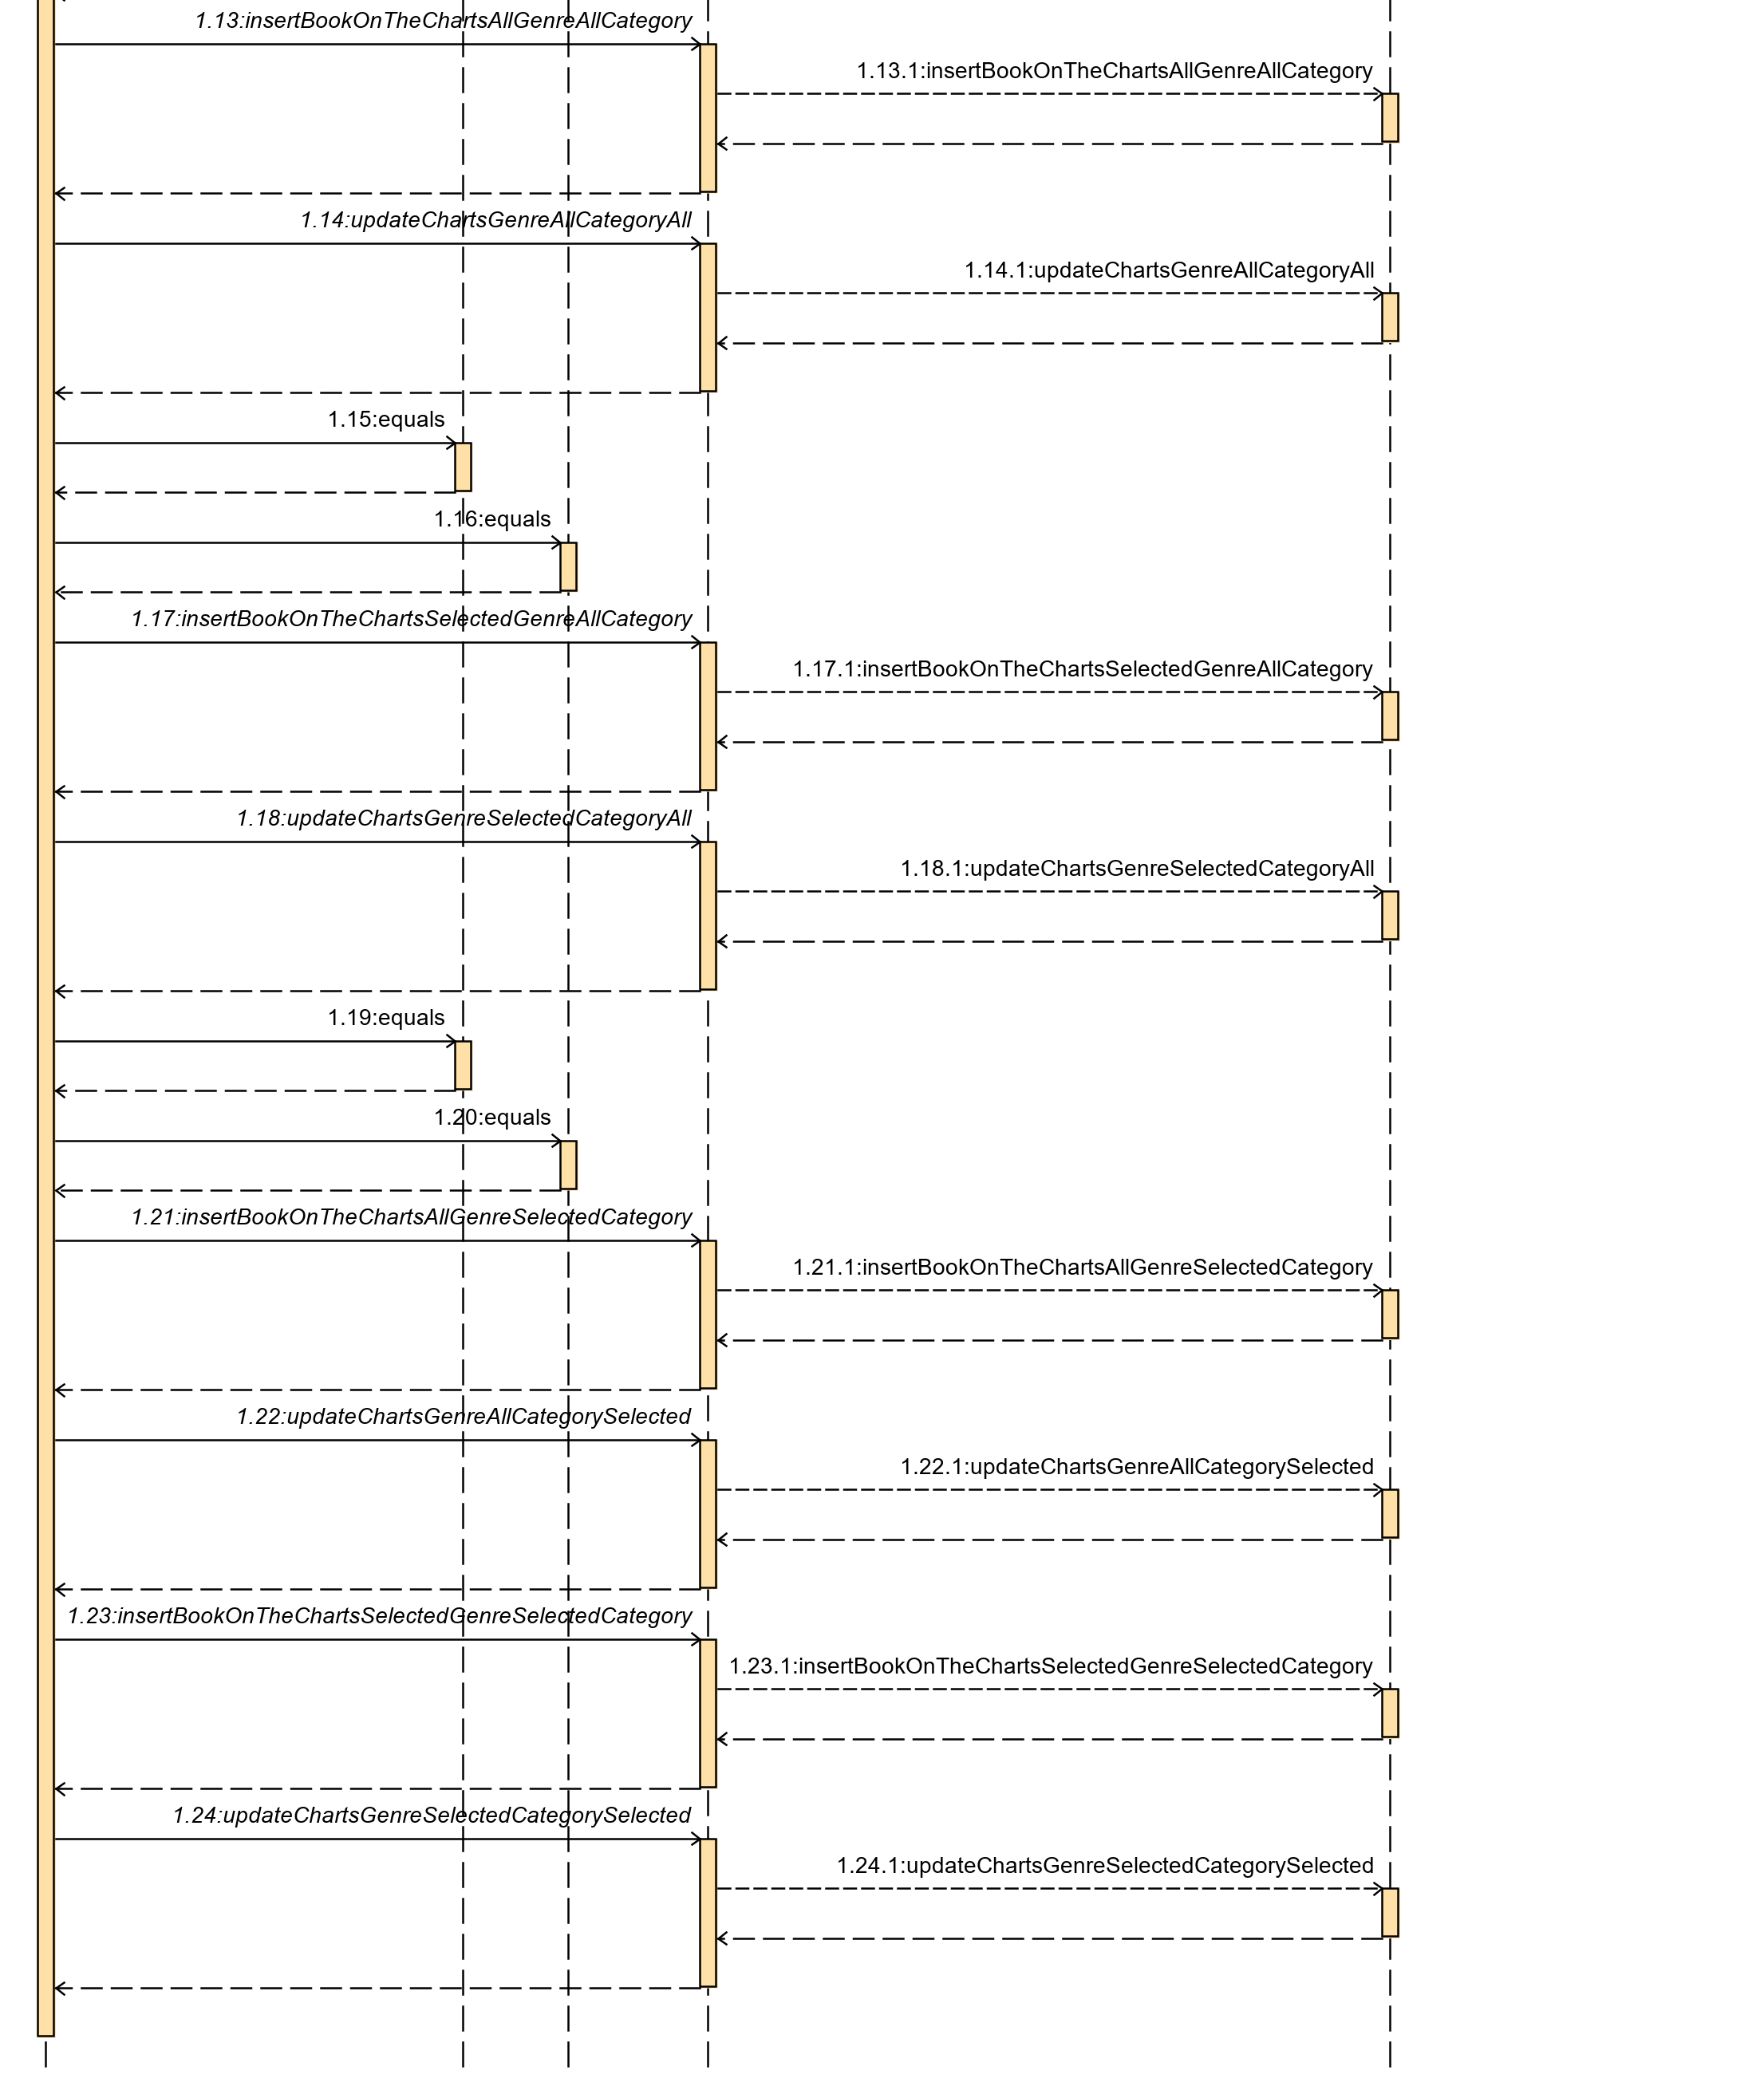
\includegraphics[width=1.2\linewidth]{Sequence diagrams/3 Manager/update2.png}
	\caption{Diagramma sequenza utente responsabile aggiorna classifiche libro}
\end{figure}

\clearpage

\chapter{Diagrammi delle attività}

Vengono ora presentati i principali diagrammi delle attività:
\section{Diagramma attività modifica dati anagrafici utente registrato}
\vspace{0.5in}
\begin{figure}[h!]
	\centering
    	\hspace*{-0.5in}
	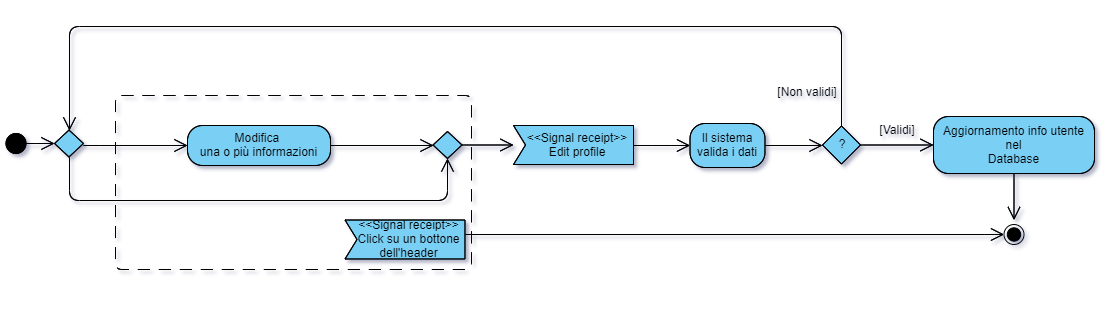
\includegraphics[width=1.3\linewidth]{Activity diagrams/activity diagram modifica indirizzo.png}
	\caption{Diagramma attività modifica dati anagrafici utente registrato}
\end{figure}
\clearpage
\section{Diagramma attività registrazione utente}
\begin{figure}[h!]
	\centering
    	\hspace*{-0.5in}
	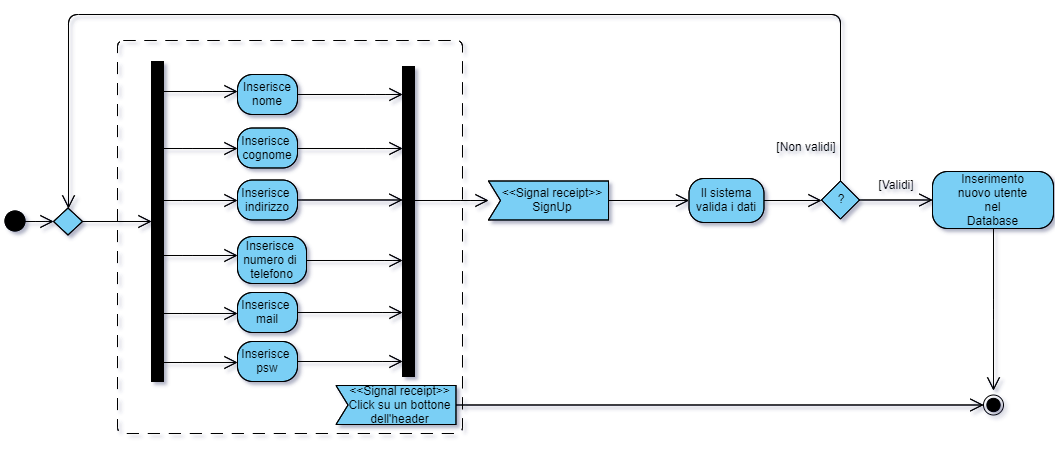
\includegraphics[width=1.1\linewidth]{Activity diagrams/activity diagram signUp.png}
	\caption{Diagramma attività registrazione utente}
\end{figure}
\section{Diagramma attività aggiunta di un libro al carrello}

\begin{figure}[h!]
	\centering
    	\hspace*{-0.5in}
	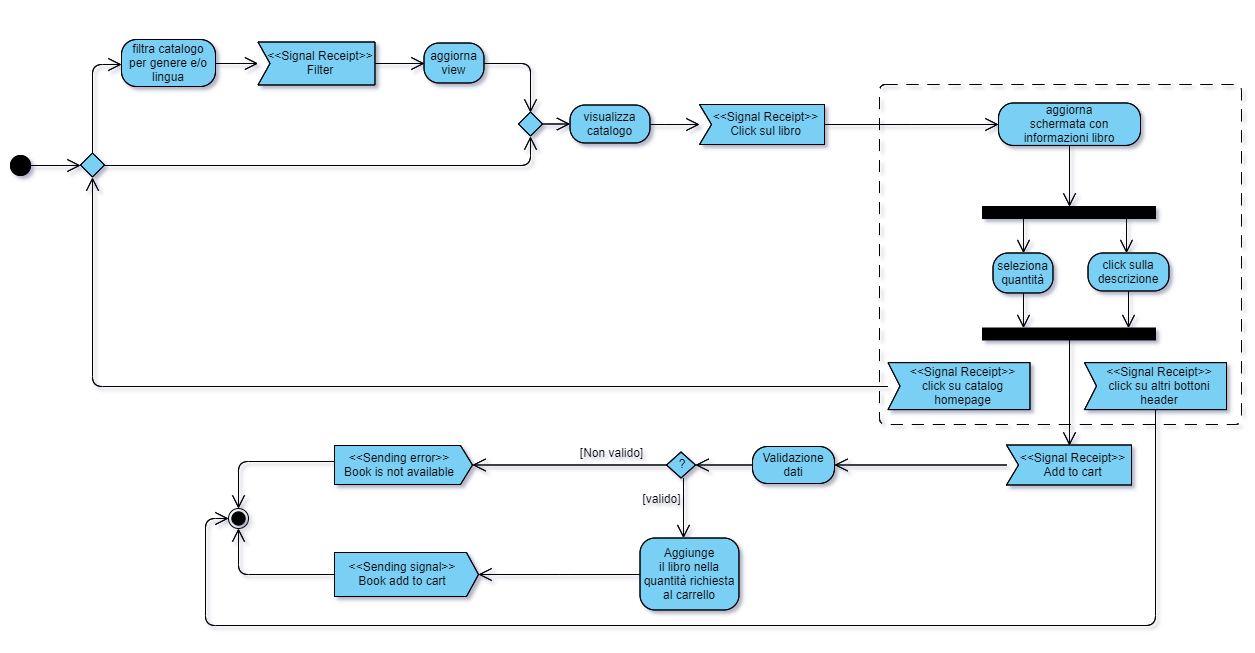
\includegraphics[width=1.3\linewidth]{Activity diagrams/addtocart.png}
	\caption{Diagramma attività aggiunta libro al carrello}
\end{figure}
\clearpage
\section{Diagramma attività creazione di un ordine}
\begin{figure}[h!]
	\centering
    	\hspace*{-0.5in}
	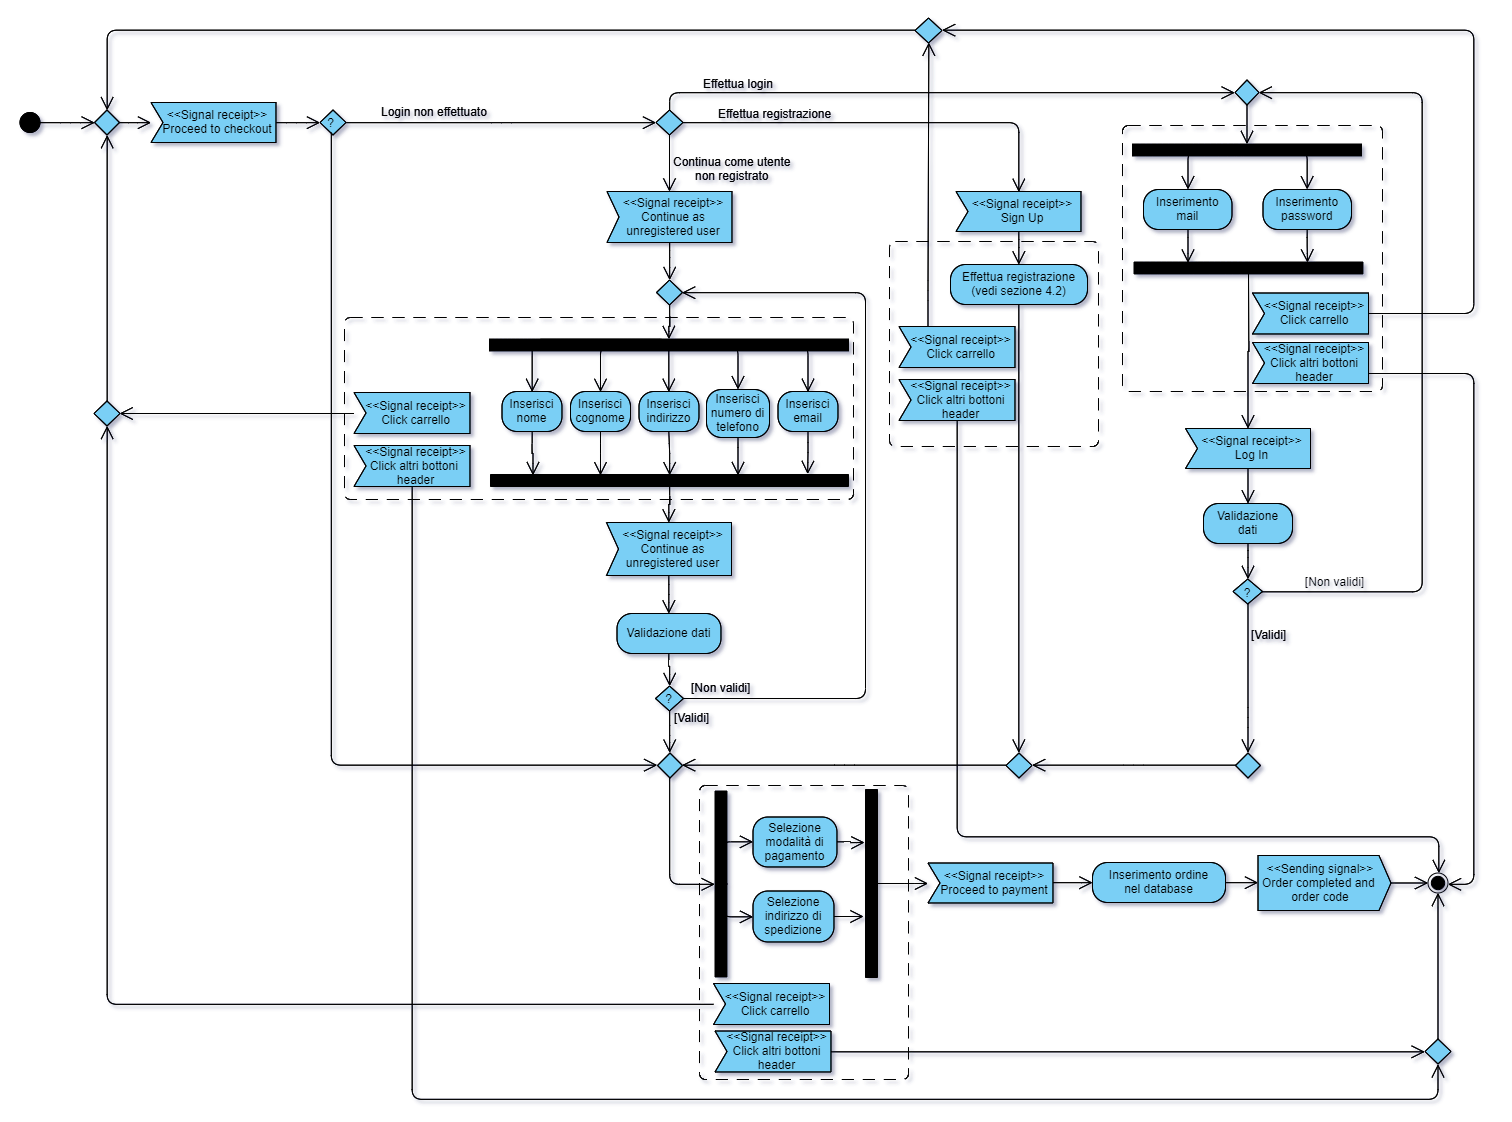
\includegraphics[width=1.3\linewidth]{Activity diagrams/Activity diagram creazione ordine.png}
	\caption{Diagramma attività creazione ordine}
\end{figure}

\clearpage

\section{Diagramma attività modifica libro catalogo}
\begin{figure}[h!]
	\centering
    	\hspace*{-0.5in}
	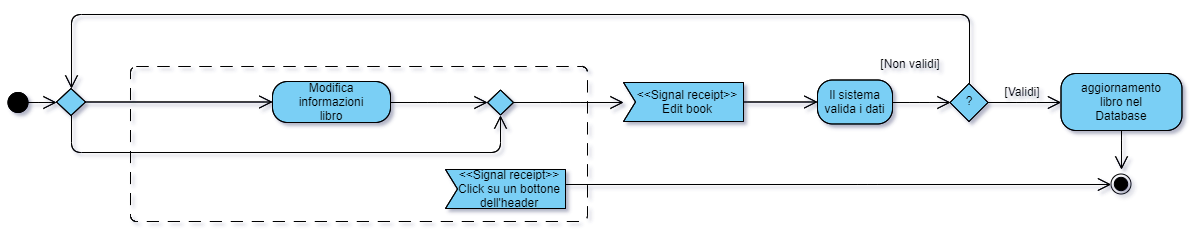
\includegraphics[width=1.3\linewidth]{Activity diagrams/editBookNew.png}
	\caption{Diagramma attività modifica libro catalogo}
\end{figure}

\section{Diagramma attività aggiunta libro al catalogo}
\begin{figure}[h!]
	\centering
    	\hspace*{-0.5in}
	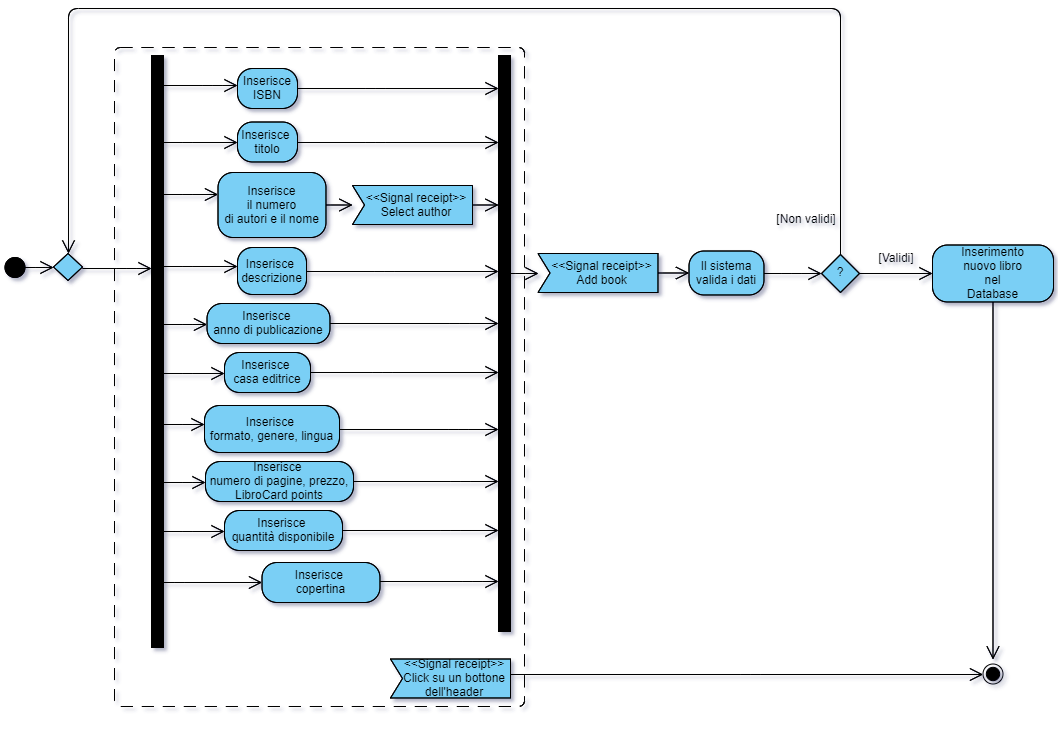
\includegraphics[width=1.3\linewidth]{Activity diagrams/addBook.png}
	\caption{Diagramma attività aggiunta libro al catalogo}
\end{figure}

\clearpage




\section{Diagramma attività aggiornamento classifiche}
\begin{figure}[h!]
	\centering
    	\hspace*{-0.5in}
	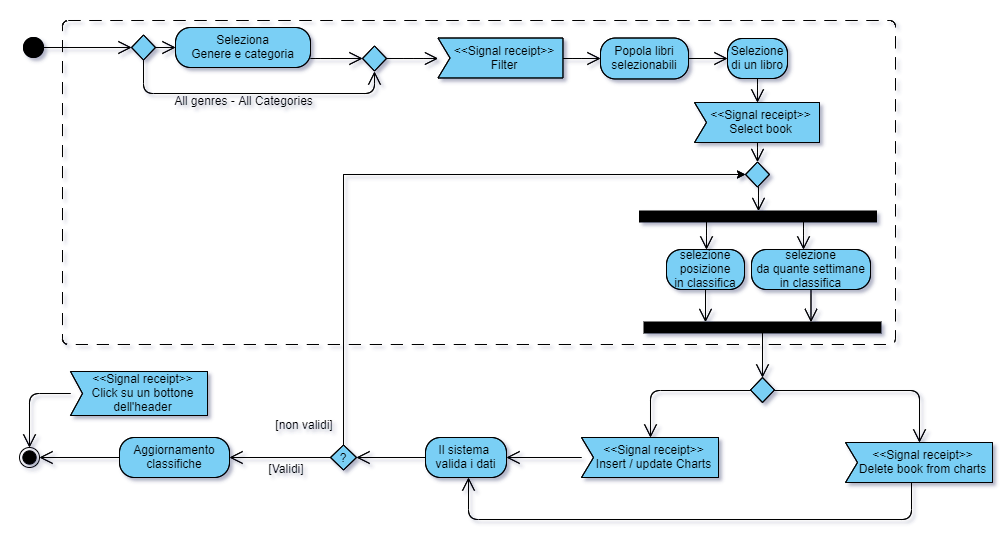
\includegraphics[width=1.3\linewidth]{Activity diagrams/updateCharts.png}
	\caption{Diagramma attività aggiornamento classifiche}
\end{figure}

\clearpage

\chapter{Diagrammi delle classi}\label{database}
Di seguito i diagrammi delle classi. \\Sono stati divisi per \textit{package} per facilitare la comprensione.

\section{Diagramma delle classi del \textit{Main}}
\begin{figure}[h!]
	\centering
	    \hspace*{-0.2in}
	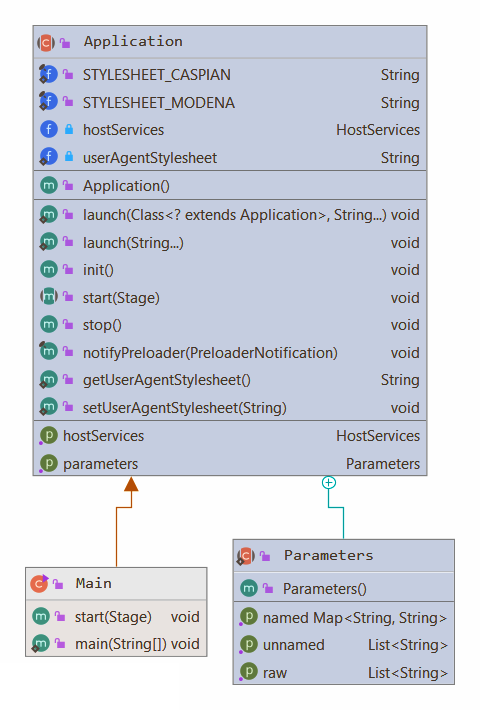
\includegraphics[width=0.5\linewidth]{Class diagrams/Main.png}
	\caption{Diagramma classe Main}
\end{figure}

\clearpage

\section{Diagramma delle classi del \textit{package Controller}}
\begin{figure}[h!]
	\centering
	    \hspace*{-0.2in}
	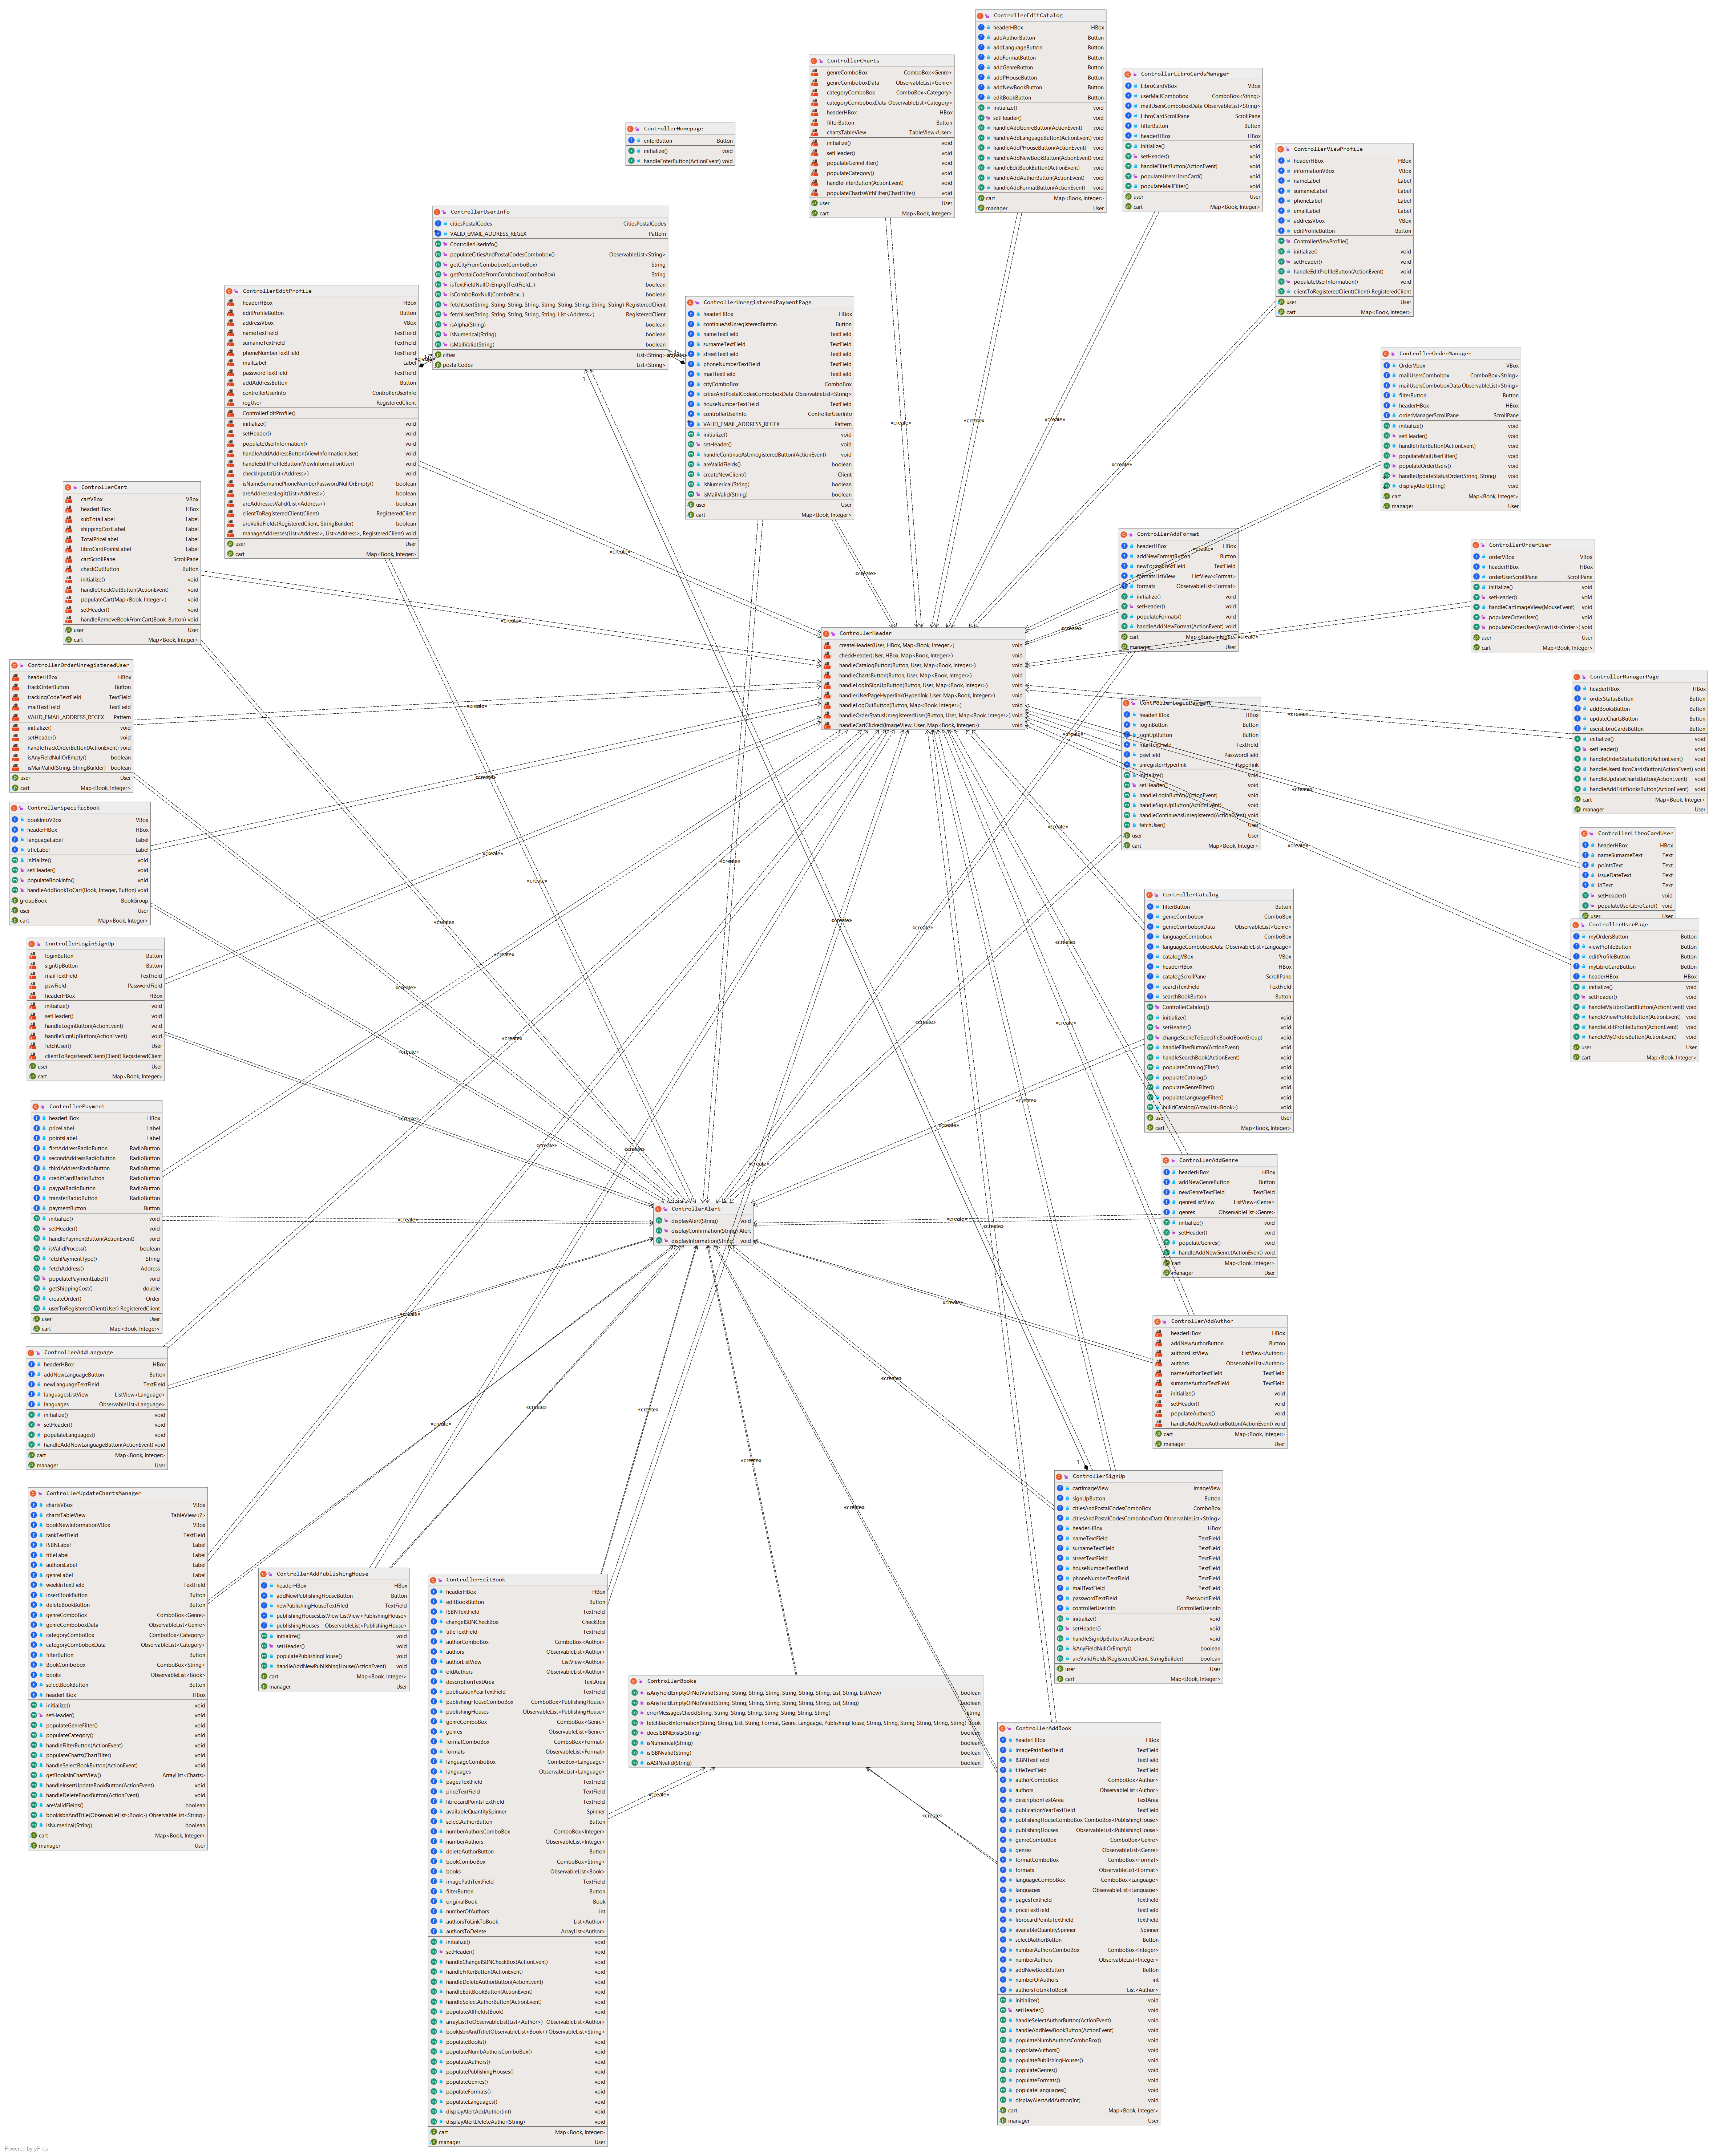
\includegraphics[width=1.15\linewidth]{Class diagrams/Package Controller.png}
	\caption{Diagramma classi Controller}
\end{figure}

\clearpage

\section{Diagramma delle classi del \textit{package Model}}\label{Model}
\begin{figure}[h!]
	\centering
	\hspace*{-0.5in}
	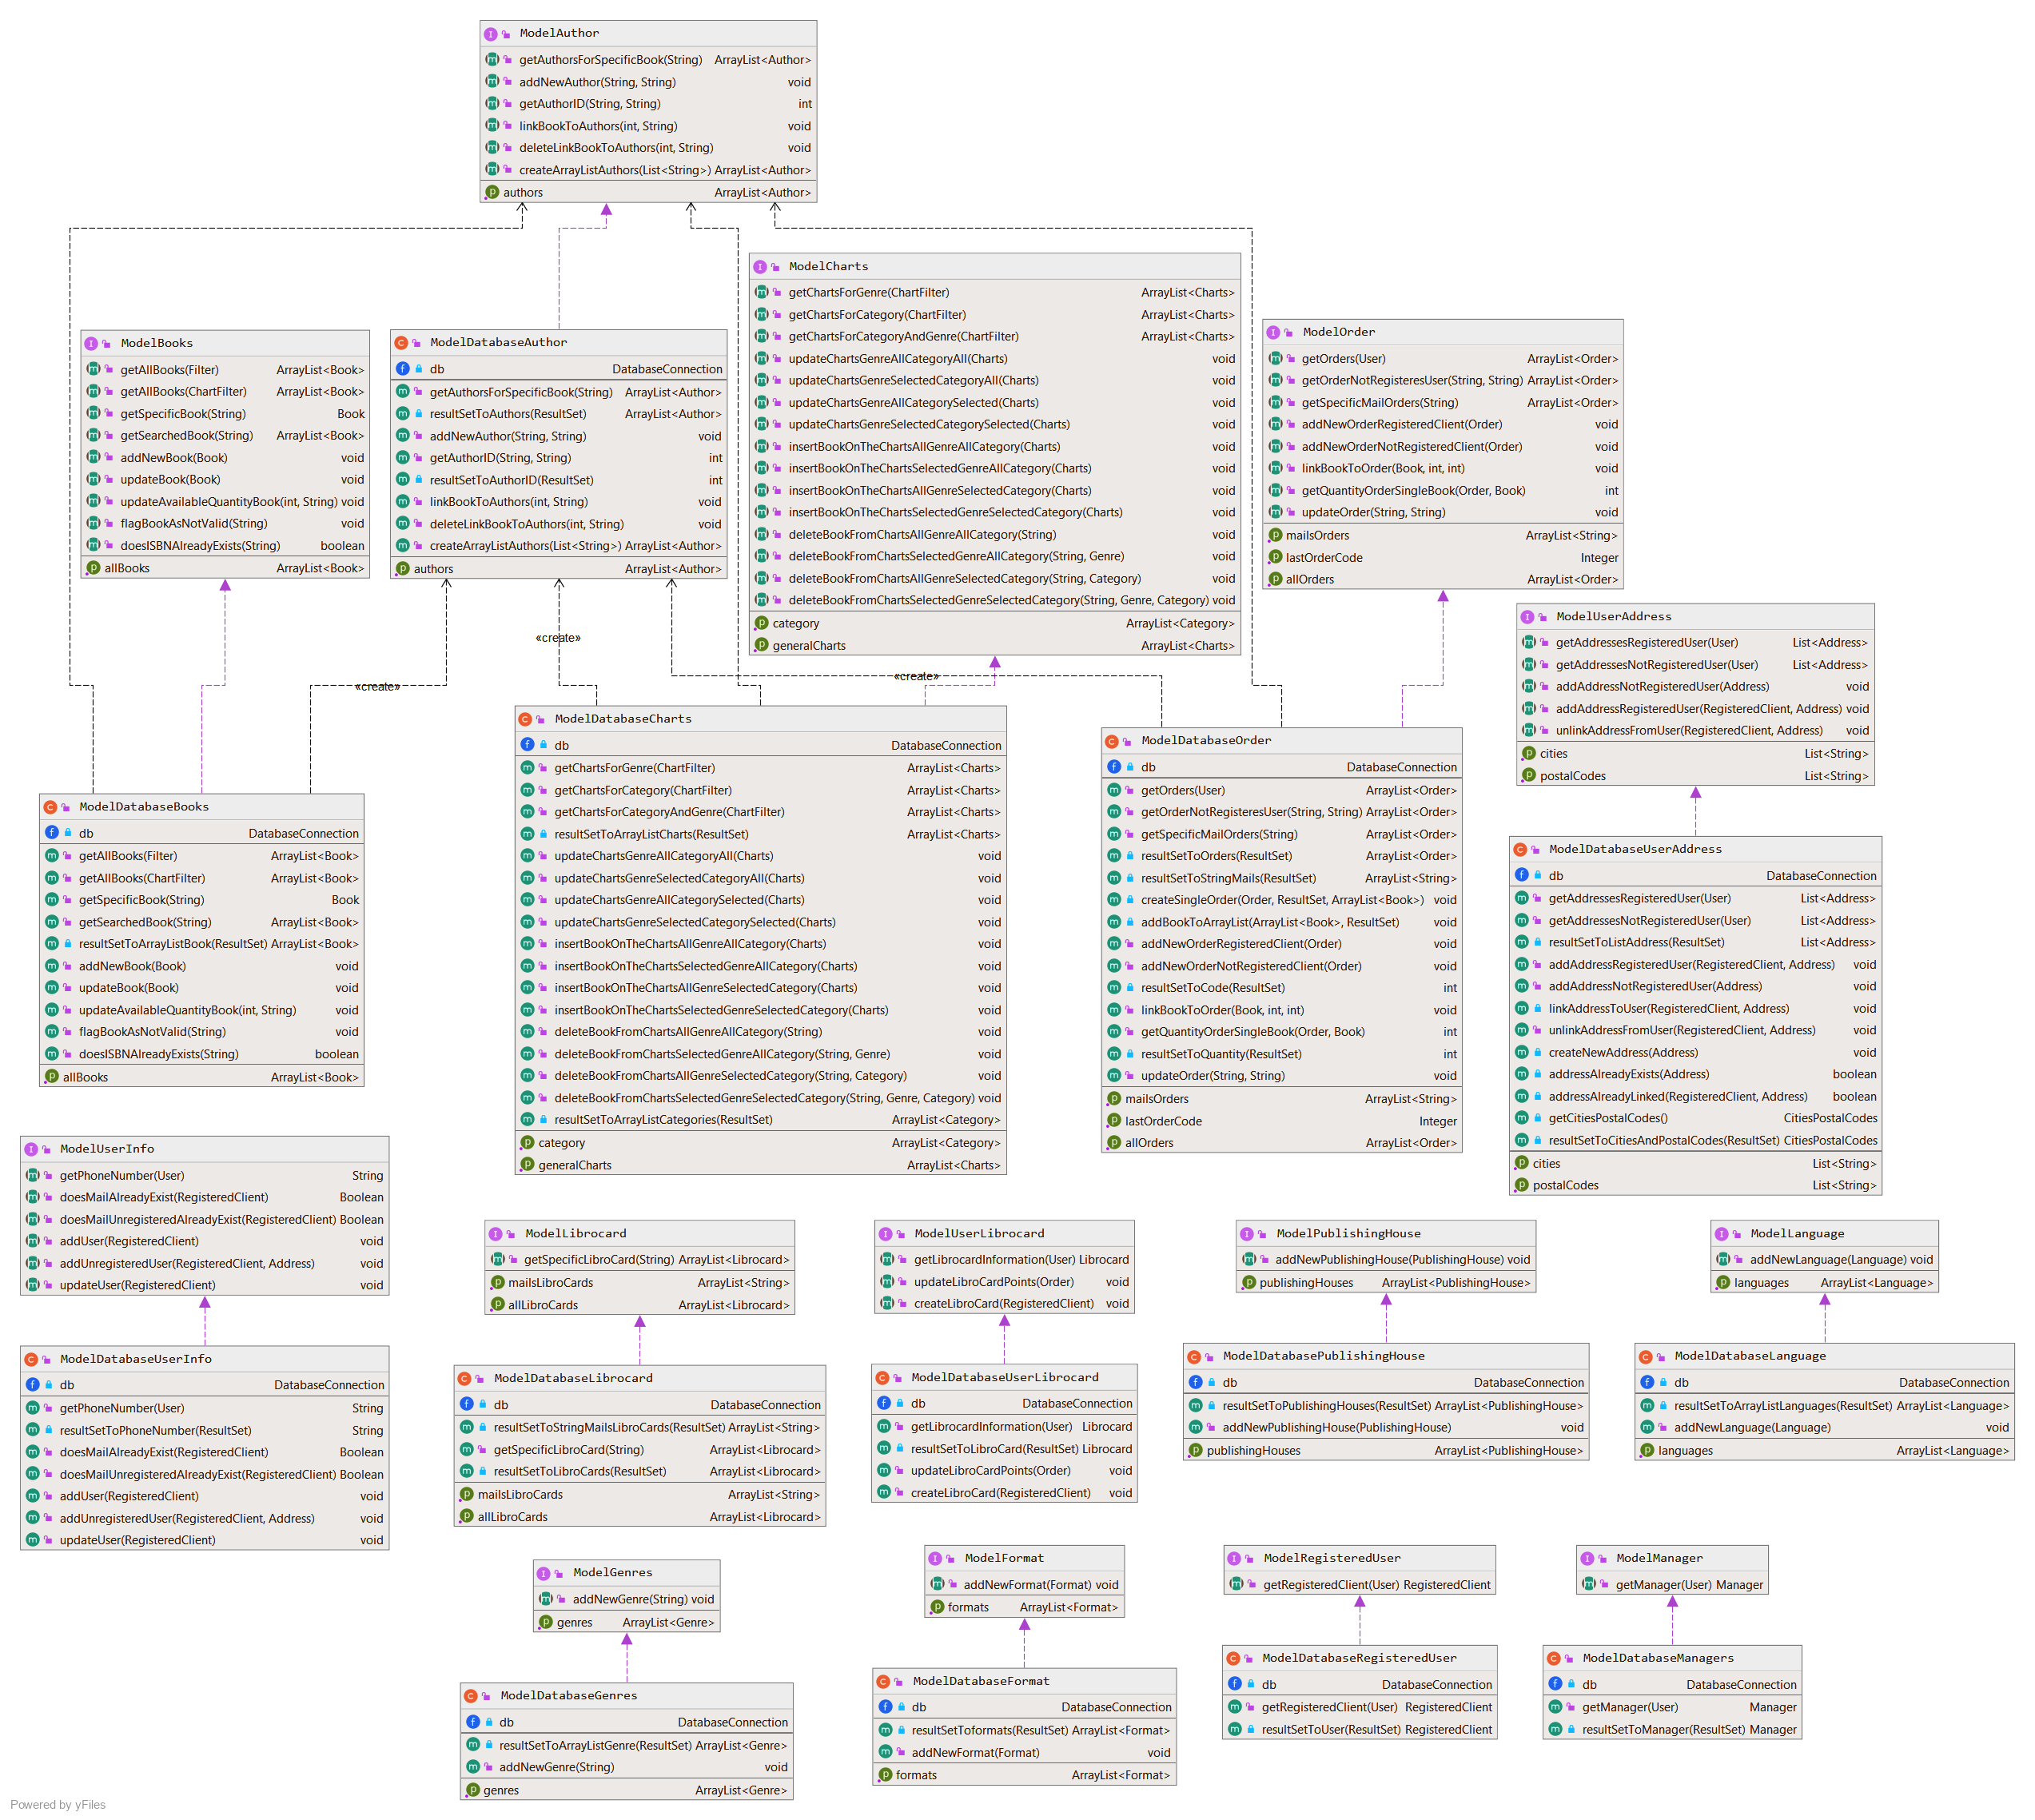
\includegraphics[width=1.3\linewidth]{Class diagrams/Package Model.png}
	\caption{Diagramma classi Model}
\end{figure}

\clearpage

\section{Diagramma delle classi del \textit{package View}}
\begin{figure}[h!]
	\centering
	\hspace*{-0.6in}
	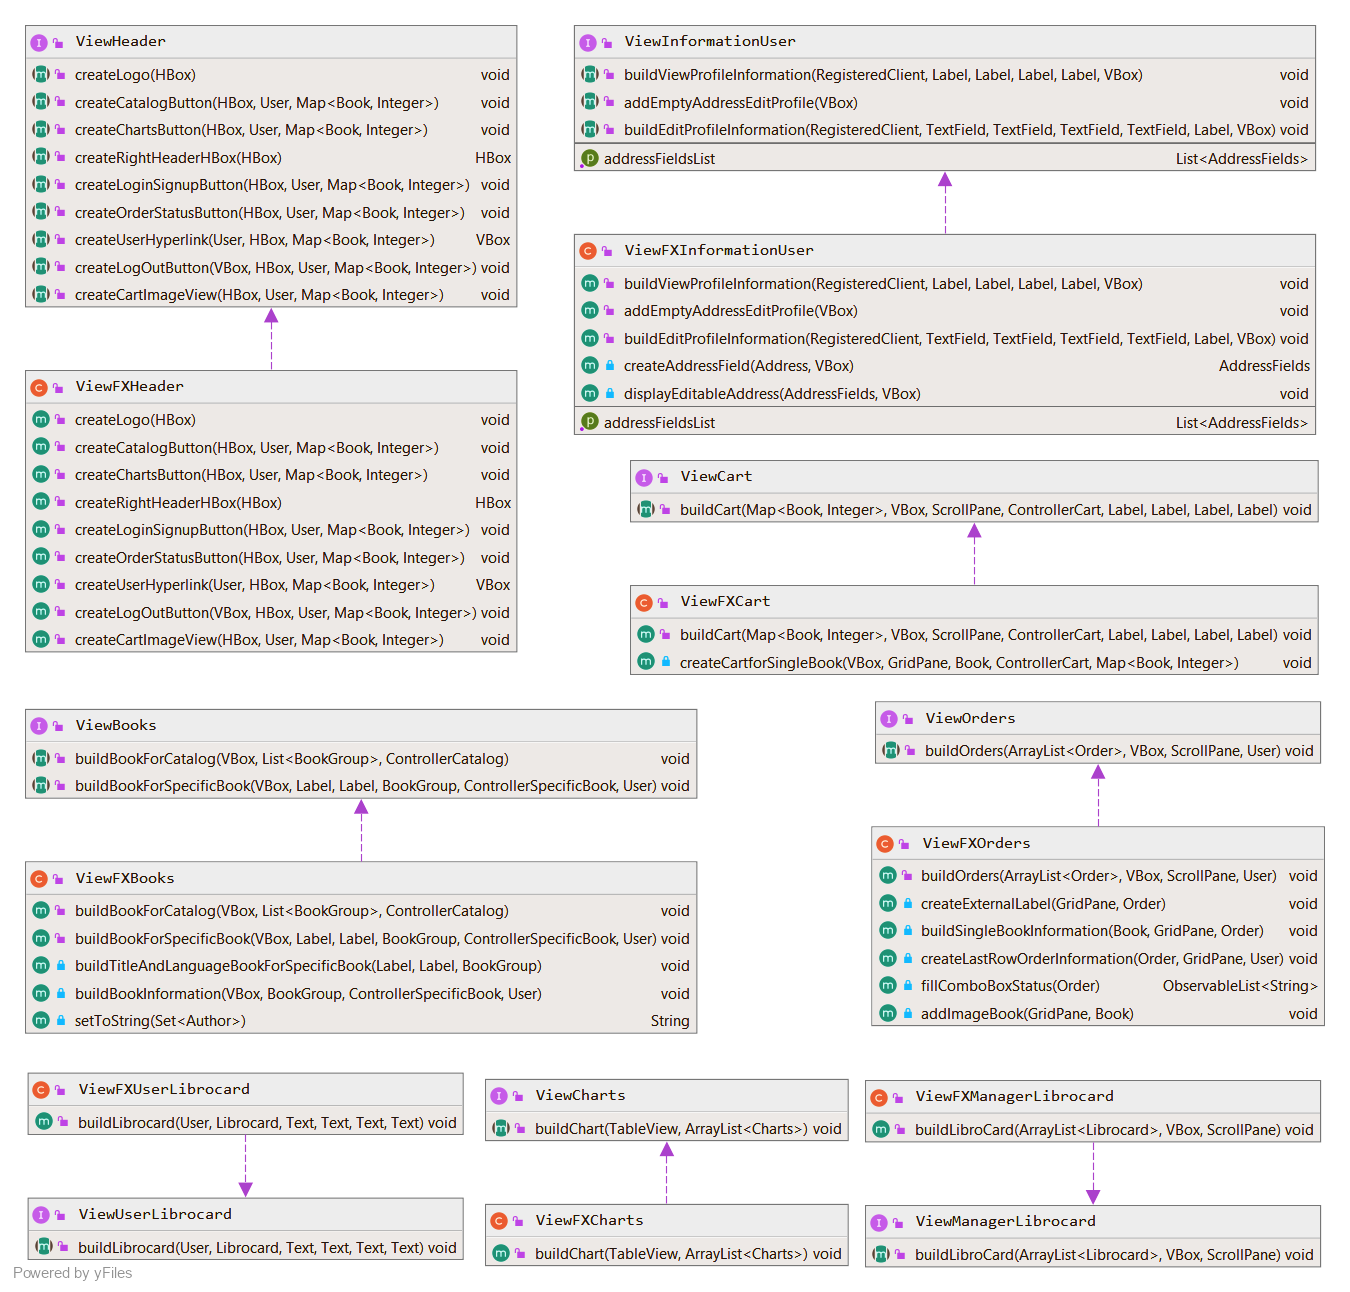
\includegraphics[width=1.3\linewidth]{Class diagrams/Package View.png}
	\caption{Diagramma classi View}
\end{figure}

\clearpage

\section{Diagramma delle classi del \textit{package Data}}
\begin{figure}[h!]
	\centering
	\hspace*{-0.8in}
	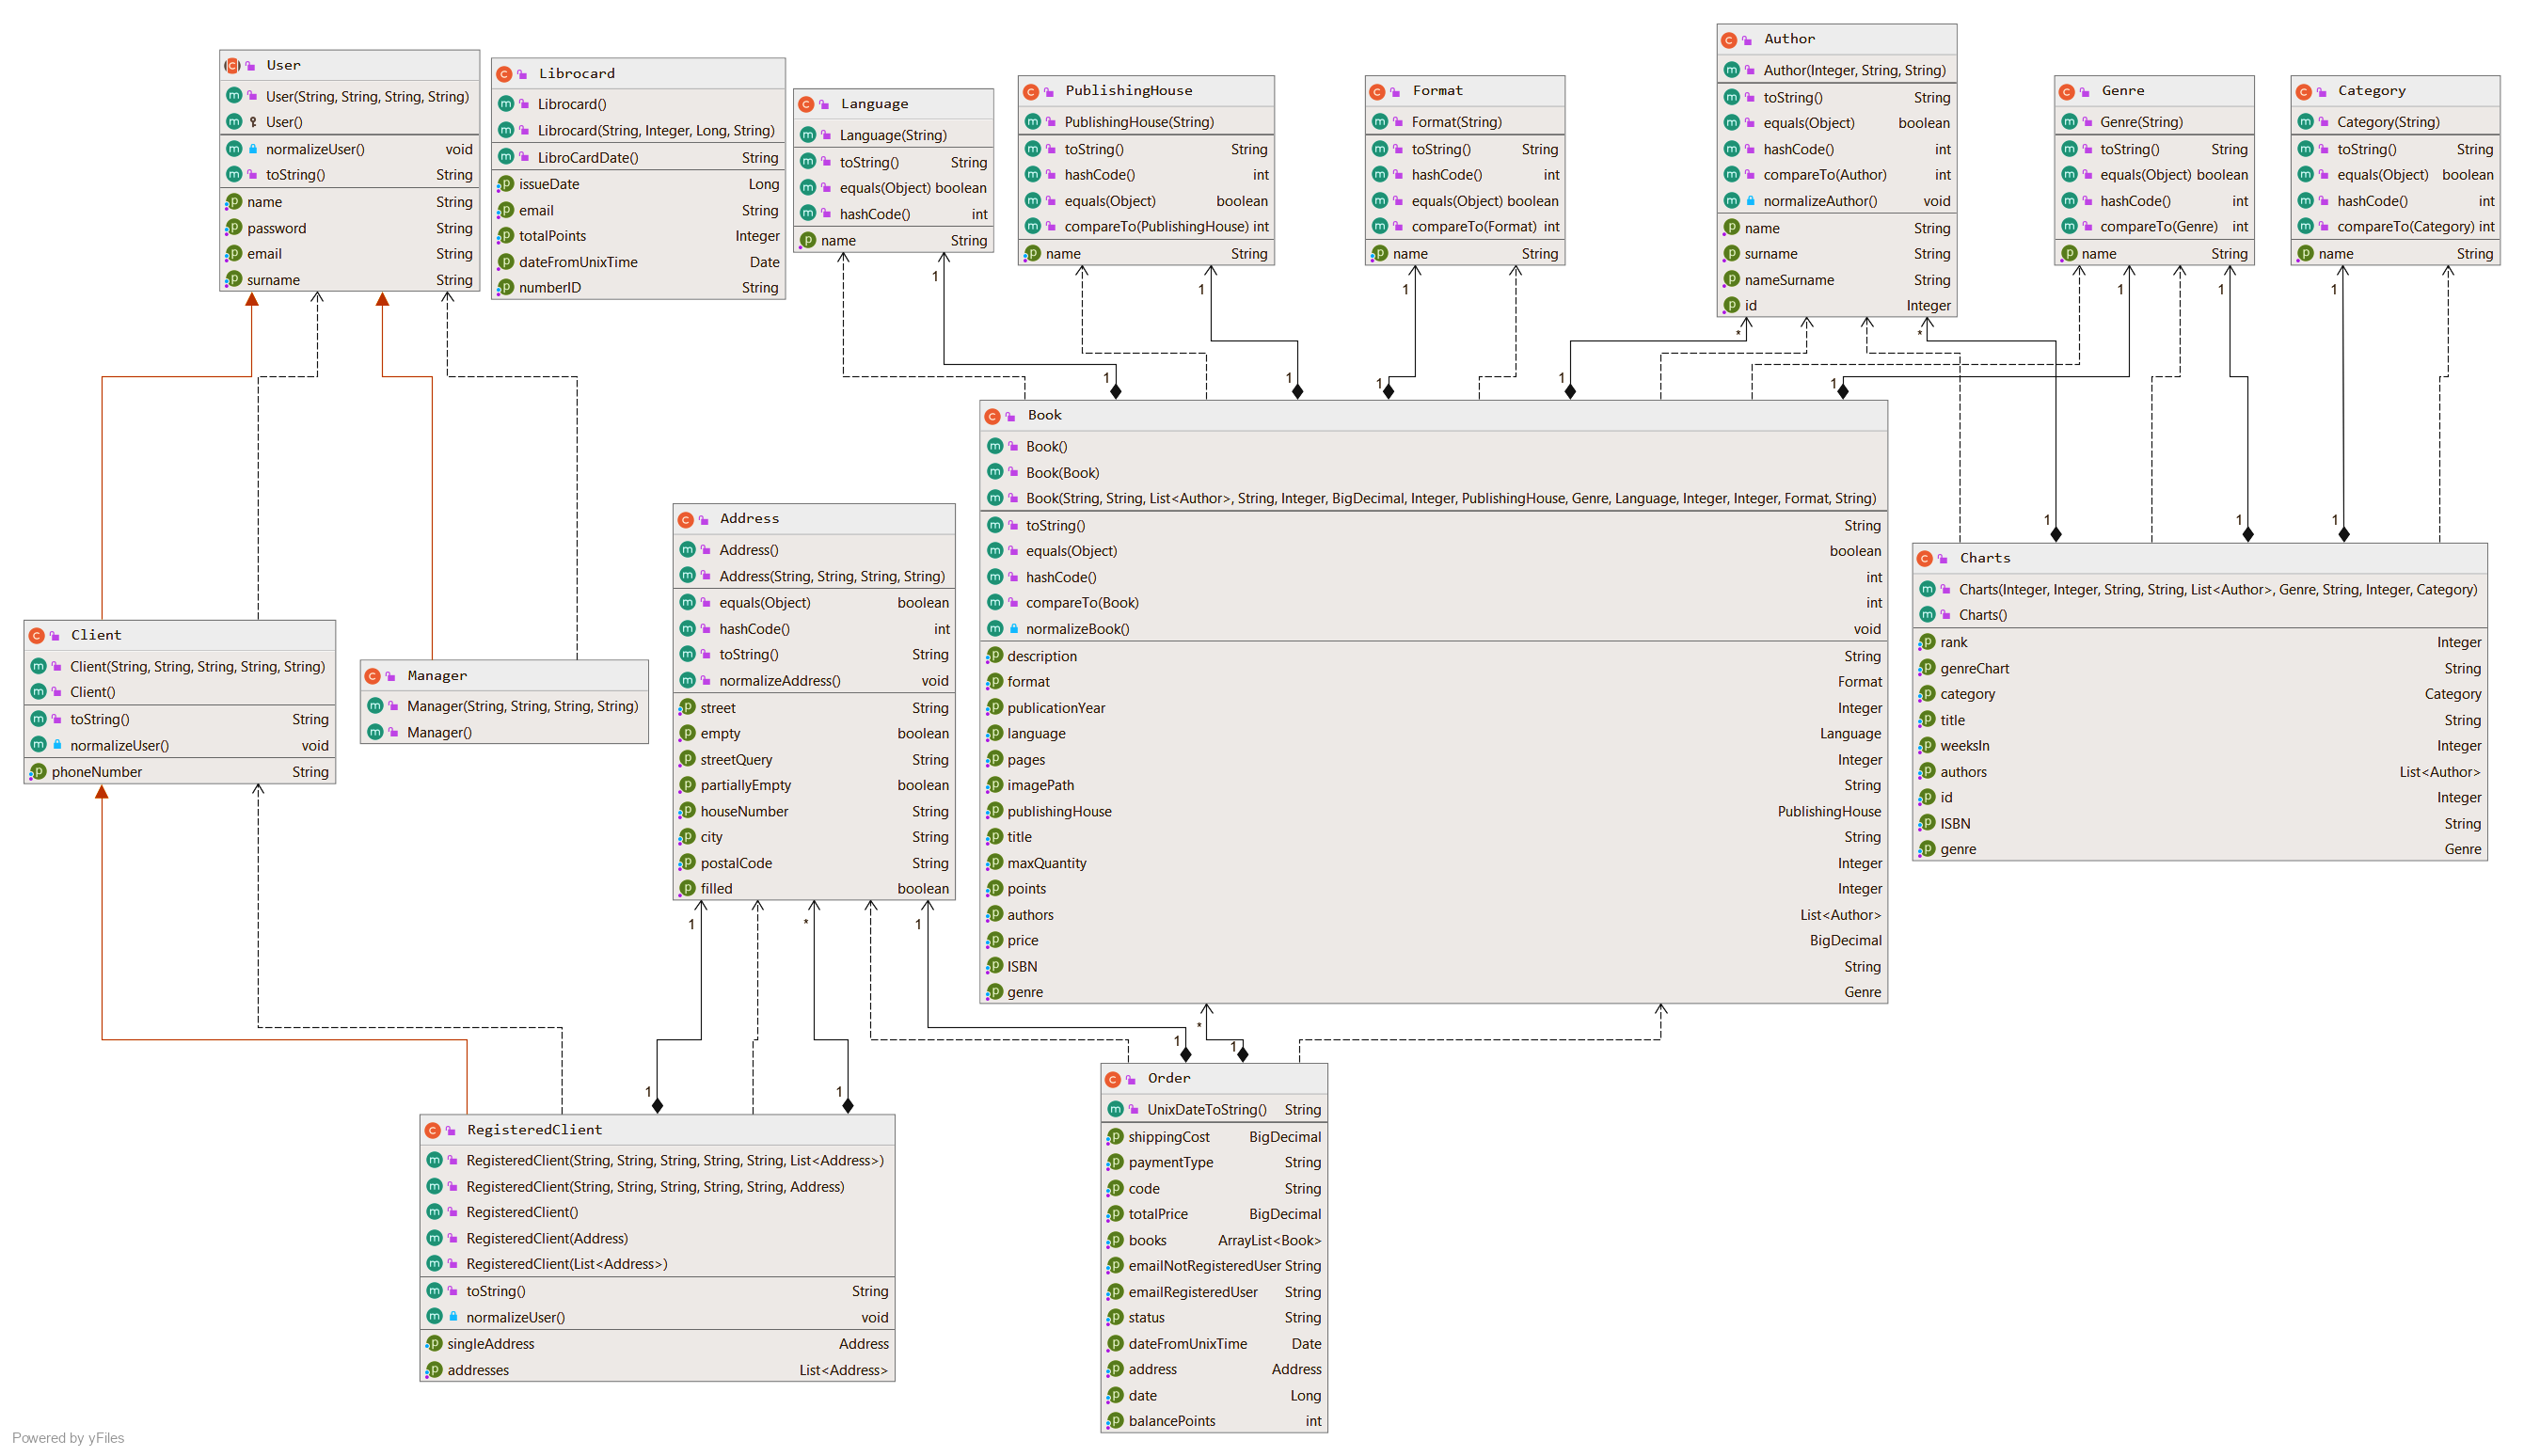
\includegraphics[width=1.3\linewidth]{Class diagrams/Package Data.png}
	\caption{Diagramma classi Data}
\end{figure}

\clearpage

\section{Diagramma delle classi del \textit{package Utils}}
\begin{figure}[h!]
	\centering
	\hspace*{-0.5in}
	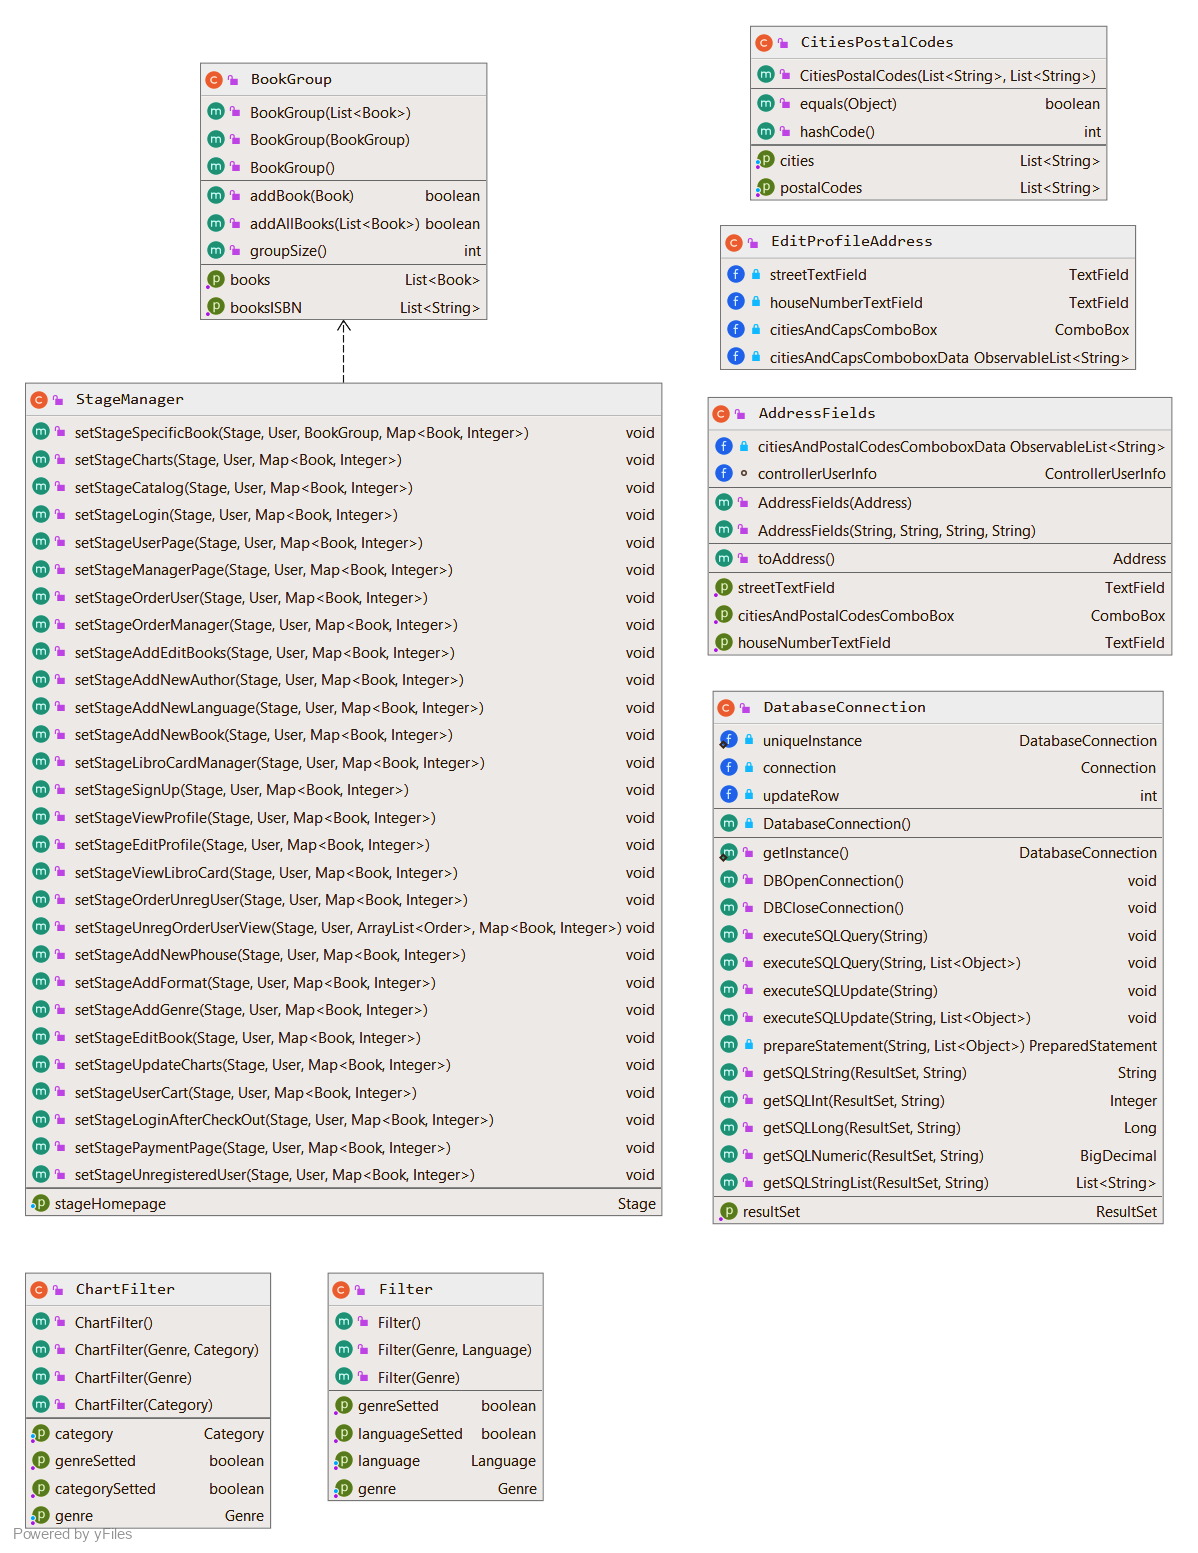
\includegraphics[width=1.1\linewidth]{Class diagrams/Package Utils.png}
	\caption{Diagramma classi Utils}
\end{figure}



\clearpage

\chapter{Struttura del database}\label{database}
\section{Scelte progettuali}

La memorizzazione delle informazioni nell'applicativo avviene utilizzando una base di dati. Si è deciso di utilizzare \textbf{SQLite} come DBMS, in quanto presenta diversi vantaggi: l'applicativo è abbastanza piccolo e l'utilizzo di SQLite è efficace, in quanto presenta funzionalità sufficienti, senza bisogno di un DBMS che invece ne implementerebbe di aggiuntive; non vi è bisogno di un collegamento remoto alla base, in quanto questa è presente come file in locale; è più facile in fase di sviluppo apportare modifiche al database se si sta lavorando in gruppo, visto che ad ogni modifica è sufficiente ricondividere il file stesso.

Di seguito sono riportate le scelte progettuali:
\begin{itemize}
    \item \textit{Generi, lingue, case editrici, formati}: si è scelto di dividere tali attributi di un libro in entità separate, in quanto è facile aggiungerne di nuovi o cambiarli per tutti i libri. Inoltre, tutti i libri utilizzano queste entità, perciò era conveniente separarle dagli altri attributi.
    
    \item \textit{Generi}: si è deciso che ogni libro potesse avere al più un genere, in quanto questo semplificava il filtraggio dei libri nel catalogo e la gestione delle classifiche. Di conseguenza, un genere può appartenere a più libri, ma un libro ha solamente un genere (cardinalità 1-N).
  
    \item \textit{Autori}: gli autori sono memorizzati in un'entità \textit{authors} separata, che ha come identificatore un attributo \textit{idAuthor}: infatti non è stato possibile utilizzare \textit{name} e \textit{surname} come identificatori, visto che vi potrebbe essere omonimia tra autori. 
    \newline
    Il collegamento tra \textit{books} e \textit{authors} è dato dall'entità \textit{write}, la quale unisce l'autore che scrive uno specifico libro. Notiamo che è possibile che un libro sia scritto da più autori, e che un autore possa scrivere più libri. Questo è possibile grazie all'utilizzo dell'entità \textit{write} (cardinalità N-N).
  
    \item \textit{Utenti}: le specifiche del progetto distinguevano l'utente in tre ruoli: utente non registrato, utente registrato e responsabili. Si è deciso di risolvere la gerarchia di utenti come accorpamento degli attributi nei figli, ottenendo perciò tre entità: \textit{notRegisteredUsers}, \textit{registeredUsers}, \textit{managers}, dove gli attributi in comune sono: \textit{email}, \textit{name}, \textit{surname}.
    \newline
    Gli attributi che \textit{notRegisteredUsers} aggiunge sono: \textit{phoneNumber}, \textit{addressStreet}, \textit{addressHouseNumber}, \textit{cityName}, \textit{cityCAP}.
    \newline
    Gli attributi che \textit{registeredUsers} aggiunge sono: \textit{phoneNumber} e \textit{password}.
    \newline
    L'attributo che \textit{manager} aggiunge è: \textit{password}.
    \item \textit{LibroCards}: la relazione che unisce \textit{libroCards} e \textit{registeredUsers} è di cardinalità 1-1. Nella risoluzione dello schema è stato quindi deciso di assegnare a \textit{libroCards} la mail dell'utente registrato come vincolo d'integrità.
    
    \item \textit{Indirizzi}: gli indirizzi sono contenuti nell'entità \textit{addresses}. Si è deciso di separare questa entità dalle altre in quanto molte entità si riferivano agli indirizzi (come per esempio \textit{orders} o \textit{notRegisteredUser}). 
    \newline
    L'entità \textit{ship} mantiene il collegamento tra indirizzi e utenti registrati, in modo che un utente registrato possa avere più indirizzi come da specifica, e che un indirizzo possa appartenere a più utenti (cardinalità N-N) 
\end{itemize}

\section{Schema Logico}
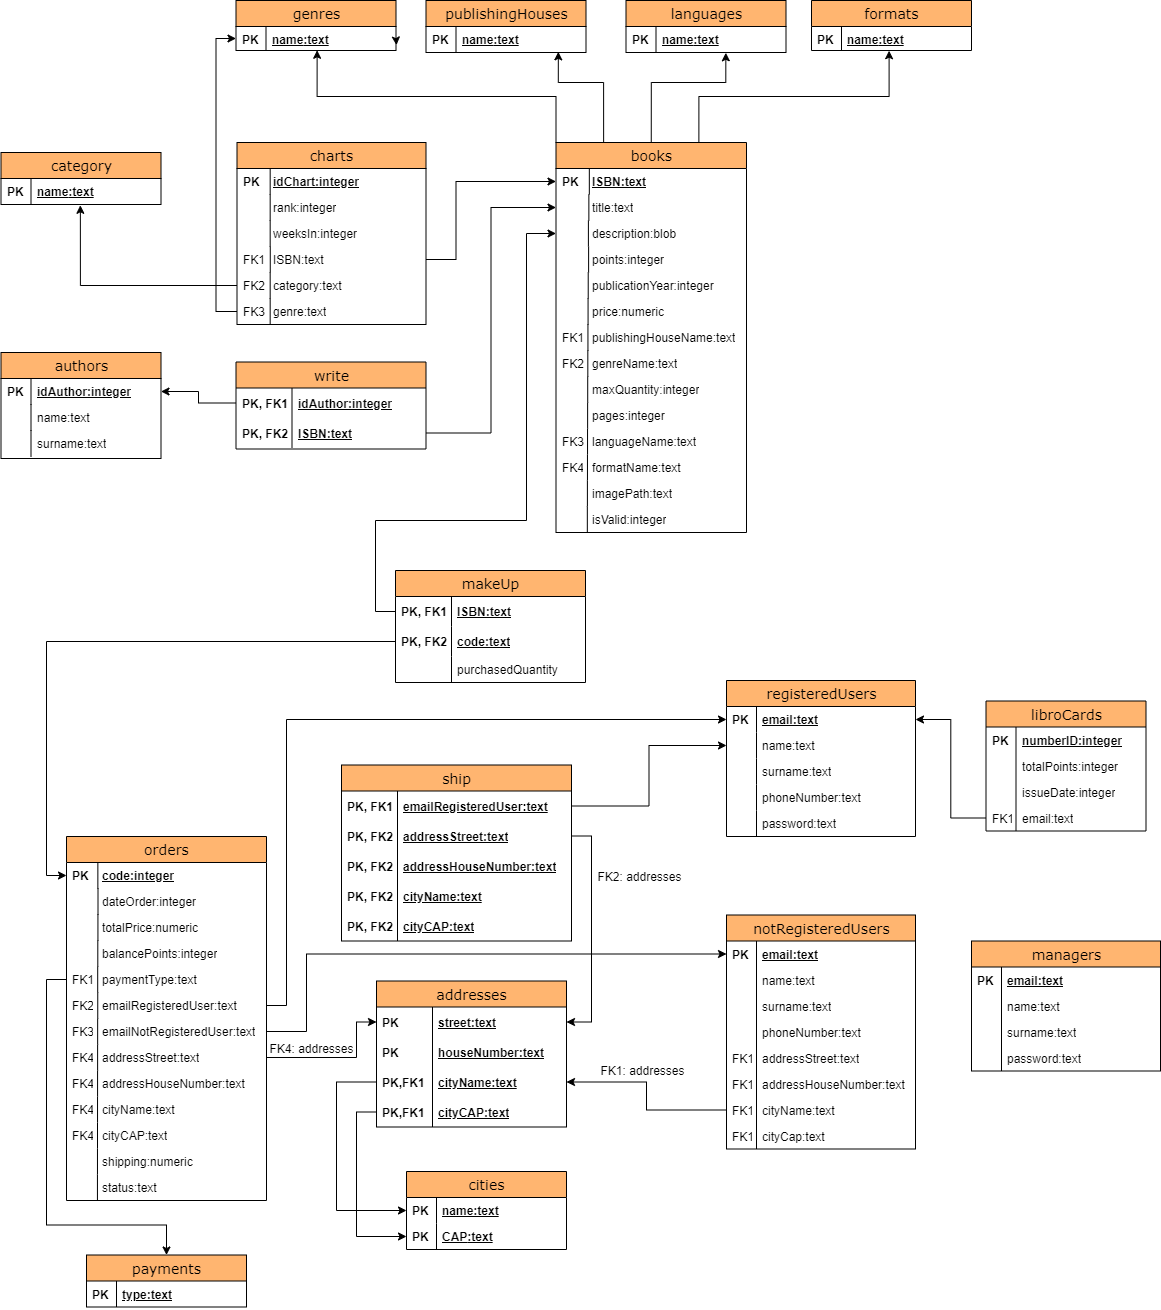
\includegraphics[width=1\linewidth]{DB diagrams/Diagramma Logico Database.png}

\section{Schema Relazionale}
I vincoli di chiave primaria sono sottolineati.

\begin{itemize}
    \item Addresses (\ul{street, houseNumber, cityName, cityCap})
    \item Authors (\ul{idAuthor}, name, surname)
    \item Books (\ul{ISBN}, title, description, points, publicationYear, price, publishingHouseName, genreName, maxQuantity, pages, languageName, formatName, imagePath, isValid)
    \item Category (\ul{name})
    \item Charts (\ul{idChart}, rank, weeksIn, ISBN, category, genre)
    \item Cities (\ul{name, CAP})
    \item Formats (\ul{name})
    \item Genres (\ul{name})
    \item Languages (\ul{name})
    \item LibroCards (\ul{numberID}, totalPoints, issueDate, email)
    \item MakeUp (\ul{ISBN, code}, purchasedQuantity)
    \item Managers (\ul{email}, name, surname, password)
    \item NotRegisteredUsers (\ul{email}, name, surname, phoneNumber, addressStreet, addressHouseNumber, cityName, cityCAP)
    \item Orders (\ul{code}, dateOrder, totalPrice, balancePoints, paymentType, emailNotRegisteredUser, emailRegisteredUser, addressStreet, addressHouseNumber, cityName, cityCAP, shipping, status)
    \item Payments (\ul{type})
    \item PublishingHouses (\ul{name})
    \item RegisteredUsers (\ul{email}, name, surname, phoneNumber, password)
    \item Ship (\ul{emailRegisteredUser, addressStreet, addressHouseNumber, cityName, cityCAP})
    \item Write (\ul{idAuthor, ISBN})
\end{itemize}
\vspace{0.4in}

\textbf{I vincoli di integrità sono}:

{
    \raggedright
    
    \begin{itemize}
        \item Addresses.cityName, Addresses.cityCAP $\rightarrow$ Cities.name, Cities.CAP
        \item Books.formatName $\rightarrow$ Formats.name
        \item Books.languageName $\rightarrow$ Languages.name
        \item Books.genreName $\rightarrow$ Genres.name
        \item Books.publishingHouseName $\rightarrow$ PublishingHouses.name
        \item Books.genreName $\rightarrow$ Genres.name
        \item Charts.ISBN $\rightarrow$ Books.ISBN
        \item Charts.category $\rightarrow$ Category.name
        \item Charts.genre $\rightarrow$ Genres.name
        \item LibroCards.email $\rightarrow$ RegisteredUsers.email
        \item MakeUp.ISBN $\rightarrow$ Books.ISBN
        \item MakeUp.code $\rightarrow$ Orders.code
        \item NotRegisteredUsers.addressStreet, NotRegisteredUsers.addressHouseNumber, NotRegisteredUsers.cityName,
        NotRegisteredUsers.cityCAP $\rightarrow$ Addresses.street, Addresses.houseNumber, Addresses.cityName, Addresses.cityCAP
        \item Orders.emailRegisteredUser $\rightarrow$ RegisteredUsers.email
        \item Orders.emailNotRegisteredUser $\rightarrow$ NotRegisteredUsers.email
        \item Orders.addressStreet, Orders.addressHouseNumber, Orders.cityName, Orders.cityCAP $\rightarrow$ Addresses.street, Addresses.houseNumber, Addresses.cityName, Addresses.cityCAP
        \item Orders.paymentType $\rightarrow$ Payments.type
        \item Ship.emailRegisteredUser $\rightarrow$ RegisteredUsers.email
        \item Ship.addressStreet, Ship.addressHouseNumber, Ship.cityName, Ship.cityCAP $\rightarrow$ Addresses.street, Addresses.houseNumber, Addresses.cityName, Addresses.cityCAP
        \item Write.idAuthor $\rightarrow$ Authors.idAuthor
        \item Write.ISBN $\rightarrow$ Books.ISBN
    \end{itemize}
}

\clearpage

\chapter{Scelte progettuali}
In questo capitolo presentiamo le scelte progettuali e i principali design pattern utilizzati al fine della realizzazione del sistema informativo richiesto.\\
\section{Sviluppo}
Abbiamo scelto di sviluppare il sistema informativo utilizzando JavaFX basato su Java in quanto è una libreria grafica relativamente recente, supportata ufficialmente e cross platform: se un domani volessimo trasferire il sistema (che in questo caso è stato sviluppato per desktop), su dispositivo mobile, potremmo farlo senza problemi in quanto l'interfaccia si adatterebbe senza incorrere in eventuali errori di visualizzazione.\\
JavaFX presenta poi ulteriori funzionalità aggiuntive rispetto a Swing, come ad esempio la possibilità di personalizzazione tramite CSS.\\
Abbiamo trovato inoltre molto utile l'utilizzo del software SceneBuilder, un designer di interfacce grafiche che è perfettamente compatibile con JavaFX.\\ Tutte le interfacce grafiche risiedono in una cartella "fxml" e sono opportunamente caricate ed elaborate in JavaFX tramite apposite classi.\\

\clearpage
\section{Metodologia di sviluppo}
Il sistema è stato interamente sviluppato usando Git (\url{https://git-scm.com/}) come sistema di versionamento del codice e GitHub (\url{https://github.com/}) per l'hosting della repository.\\
Il sistema è stato sviluppato utilizzando una metodologia \textbf{Agile}: dopo aver analizzato i requisiti abbiamo deciso di suddividere la progettazione in macro aree: 
\begin{itemize}
    \item una prima area inerente allo memorizzazione dei dati, quindi ci siamo concentrati sullo sviluppo del database presentato al capitolo \ref{database}
    \item successivamente abbiamo analizzato con attenzione la parte logica e user interface, al fine di rispettare al meglio i requisiti.
\end{itemize} 
Quest'ultimo punto è stato a sua volta suddiviso in task brevi che rispecchiassero le singole schermate sulle quale l'utente poi andava ad interagire.\\ Avendo diviso il lavoro in task relativamente brevi, è risultato semplice testare e verificare immediatamente il corretto funzionamento di quanto implementato. \\
\newline 
I design pattern, presentati nel prossimo paragrafo \ref{design patter}, sono stati decisi in fase di sviluppo del progetto e adattati al meglio alle caratteristiche richieste dal software.\\ 
In alcune occasioni è stato necessario un refactoring del codice al fine di migliorare la pulizia, la correttezza e le prestazioni del software. \\
Quest'ultimo punto è stato semplificato grazie all'utilizzo di diverse branch su GitHub, che ci hanno permesso di mantenere una cronologia delle modifiche eseguite e eventualmente scartare quelle ritenute non corrette.\\
\begin{figure}[h!]
    	\centering
    	\hspace*{-0.5in}
    	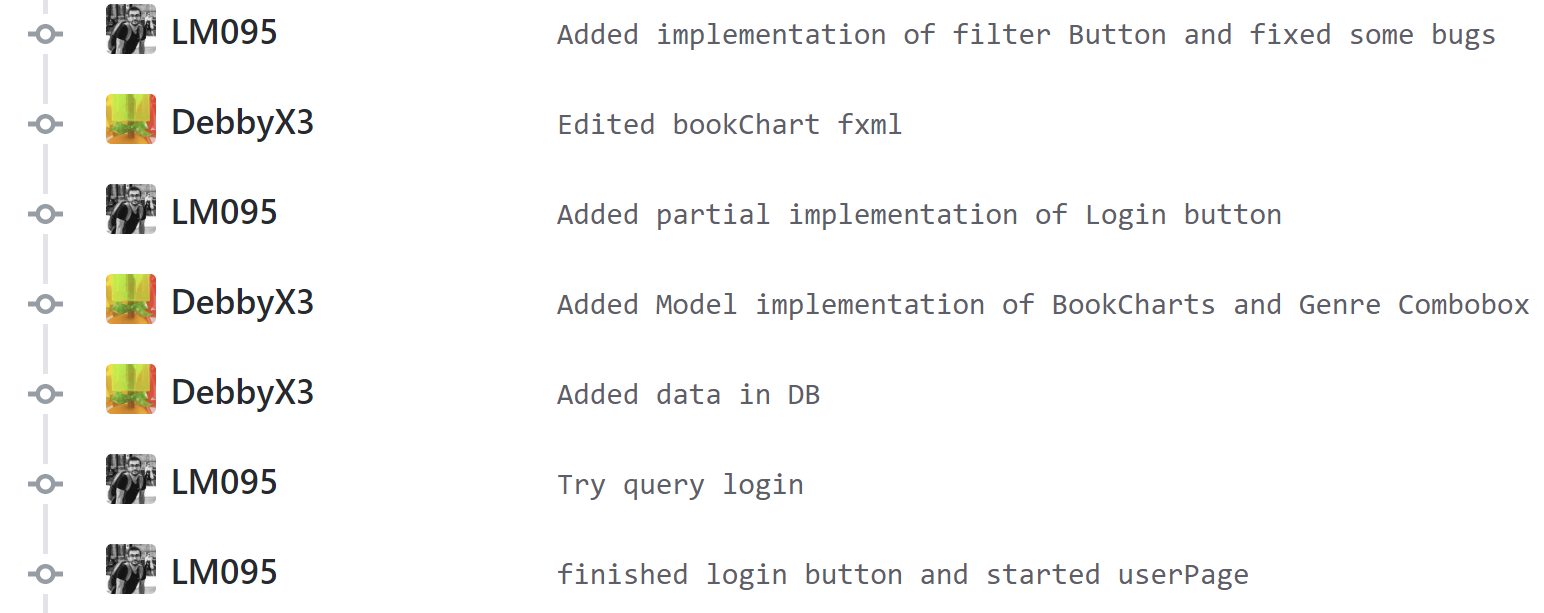
\includegraphics[width=0.8\linewidth]{Other/esGitHub.PNG}
    	\caption{esempio interazione GitHub}
    \end{figure}\\

\section{Design Pattern utilizzati}\label{design patter}
Vengono presentati in questa sezione i principali pattern utilizzati.\\
Sono inoltre presentate le varie difficoltà incontrate e soluzioni adottate per la realizzazione degli stessi.\\
\subsection{MVC pattern}
Lo schema architetturale scelto per l’applicazione è quello del \textbf{MVC} (Model-View-Controller).\\
Come presentato nel Diagramma delle Sequenze e delle Classi, le tre componenti di questo pattern comunicano tra loro.\\ 
La View genera eventi che vengono mandati al Controller corrispondente, il quale contiene la logica applicativa: questo decide, infatti, se interfacciarsi con il Model, per richiedere o salvare dati, oppure se comandare altre azioni alla View. \\
Schematicamente possiamo vedere il flusso dell'esecuzione come segue:\\
    \begin{figure}[h!]
    	\centering
    	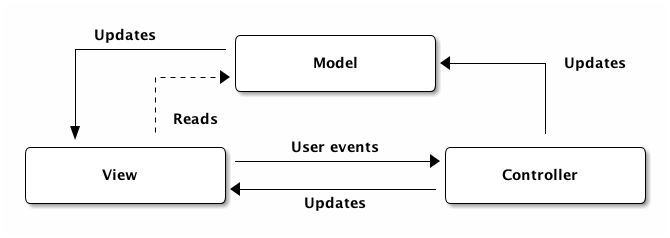
\includegraphics[width=1\linewidth]{Other/mvc.png}
    	\caption{MVC design pattern}
    \end{figure}\\
Possiamo notare che, in alcuni casi, la View si interfaccia direttamente con il Model per recuperare delle informazioni al fine di aggiornare la View, in tutti gli altri casi però, è il Controller a fare da "ponte" tra Model e View.\\
Nel nostro progetto abbiamo tutti questi possibili casi implementati.\\
\clearpage

\subsection{Facade pattern}
Al fine di nascondere la complessità computazionale del DB, inizialmente avevamo deciso di utilizzare il \textbf{Facade} come pattern per la gestione dei\\ Model.\\
Tuttavia non è stato possibile utilizzare questo pattern in quanto, avendo parecchi metodi e classi Model specifici per ogni esigenza, avremmo avuto il seguente problema: creando un'unica interfaccia Model con all'interno tutti i metodi non implementati, ogni volta che si creava una classe concreata "ModelSpecifico", quest'ultima era costretta, per definizione di implementazione di interfaccia, ad implementare, tramite Override, tutti i metodi dell'interfaccia Model, anche se quei metodi non la interessavano.\\
La soluzione allora sarebbe stata quella di non fare l'Override dei metodi non interessati e lasciare quindi il metodo di "default" dell'interfaccia. Quest'ultima soluzione però risulta, in primis poco corretta e successivamente soggetta a potenziali generazioni di errori nel codice.
\newline

Viene riportato un esemplificazione del problema riscontrato.

Seguendo la struttura standard del facade pattern avremmo dovuto avere una struttura analoga:\\
     \begin{figure}[h!]
    	\centering
    	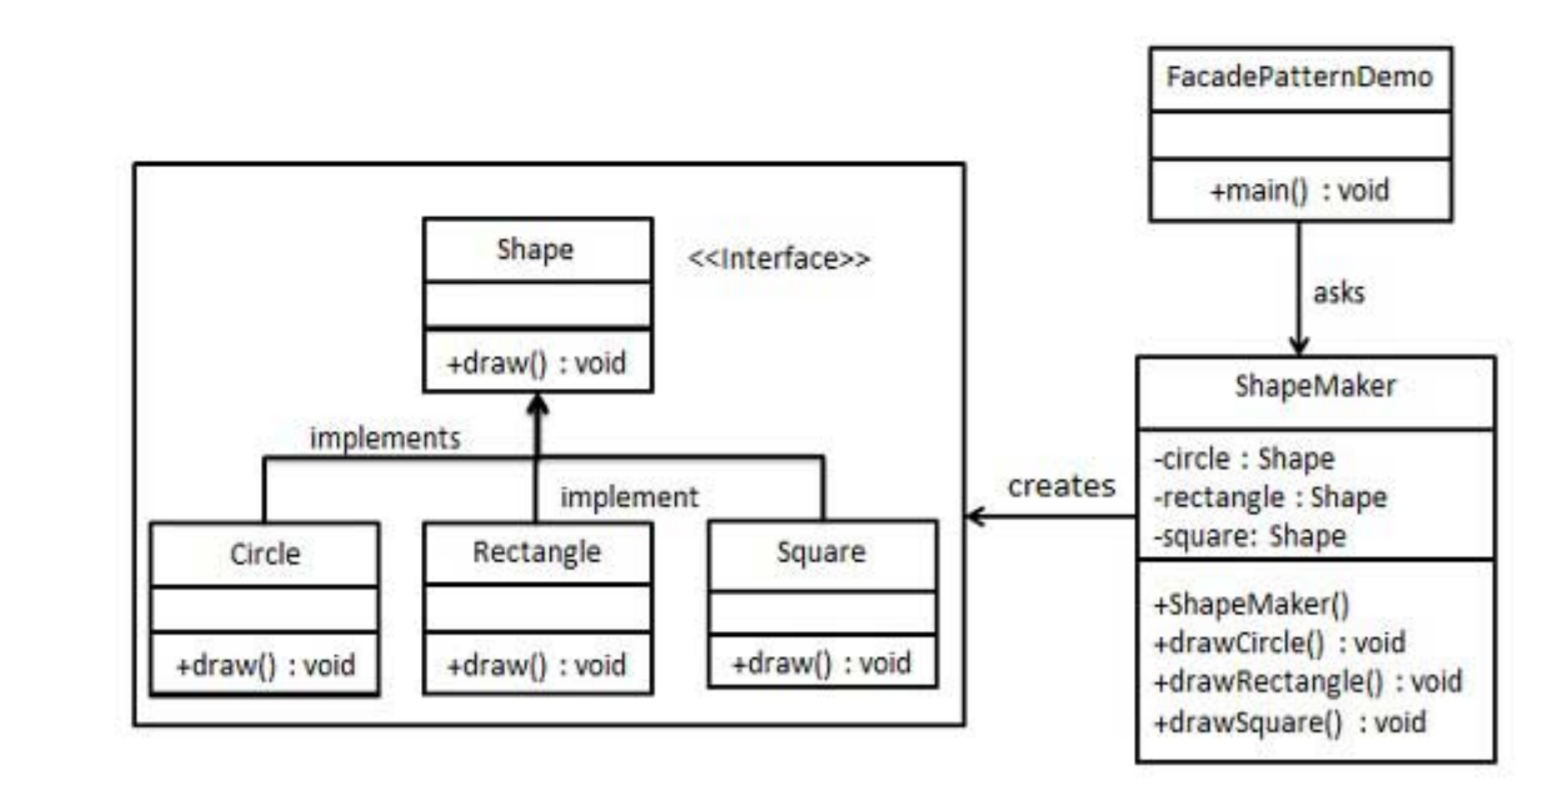
\includegraphics[width=1\linewidth]{Other/schema facade.PNG}
    	\caption{Struttura facade}
    \end{figure}\\
\clearpage

Dove sostanzialmente la nostra interfaccia Model era:\\
\begin{figure}[h!]
    	\centering
    	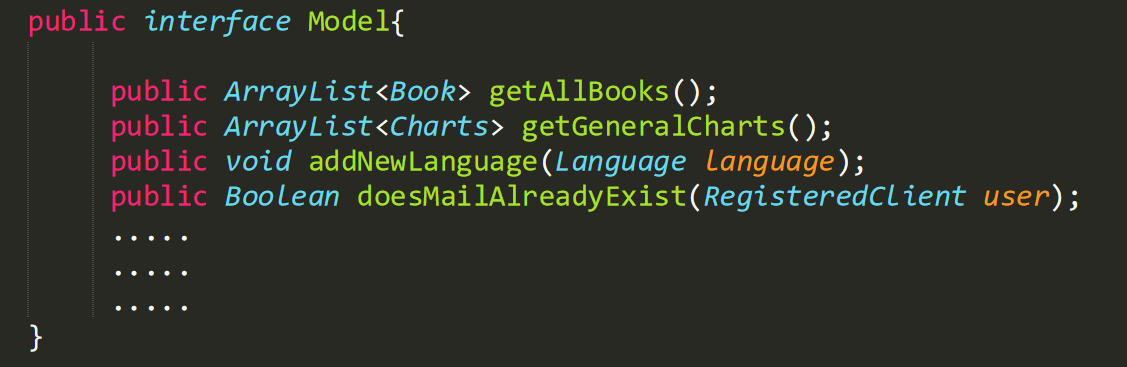
\includegraphics[width=1\linewidth]{Other/interfaccia.PNG}
    	\caption{esempio possibile interfaccia progetto}
    \end{figure}\\

e le varie classi concrete erano:\\
\begin{figure}[h!]
    	\centering
    	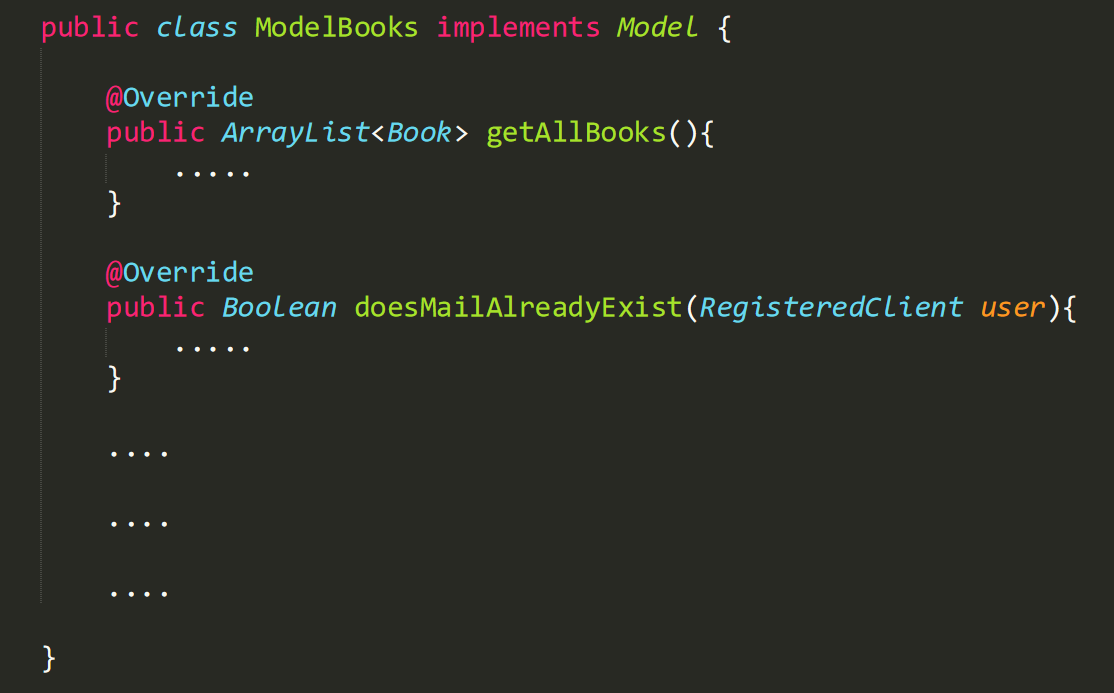
\includegraphics[width=1\linewidth]{Other/classe.PNG}
    	\caption{esempio possibile interfaccia progetto}
    \end{figure}\\

Il problema sopra menzionato è ben visibile nell'immagine qui sopra riportata: avere un'unica interfaccia con tutti i metodi inerenti all'utilizzo del database non era possibile. Infatti, le varie classi concrete avrebbero dovuto implementare, tramite Override, anche metodi non specifici per quella determinata classe, come ad esempio il metodo "doesMailAlreadyExist" nell'immagine sopra, che riguarda ModelUser piuttosto che ModelBook.\\

Era possibile non implementare il metodo che non interessa direttamente la classe, ma questo risulta essere, come già detto in precedenza, poco corretto (visto che si sarebbe dovuto scrivere un metodo \textit{default} vuoto nell'interfaccia) e soggetto a possibili errori a runtime.\\

La soluzione a questo problema quindi è l'implementazione del pattern DAO, a cui si rimanda.

\subsection{DAO pattern}
I Model seguono l'implementazione base del pattern \textbf{DAO} (Data Access Object).\\ 
Il pattern DAO risulta particolarmente adatto, in quanto è stato pensato appositamente per accedere a dati persistenti. Visto che l'accesso alle informazioni dipende dalla sorgente nella quale sono conservate, e dal tipo di memorizzazione (file, database relazionali oppure object-oriented), il pattern DAO ne astrae e incapsula l'accesso, in modo che le altri classi non sappiano con che tecnologia sono memorizzate. Inoltre, gestisce la connessione con la sorgente per ottenere e memorizzare i dati.
\newline
Le classi utilizzate per implementare il pattern sono di tre tipi: 
\begin{itemize}
    \item una classe di tipo \textit{entity}, che contiene tutte le informazioni del dato da prelevare o memorizzare;
    \item una classe di tipo \textit{Model interface}, la quale funge da interfaccia verso l'esterno. Non importa che tecnologia si sta usando per prelevare l'informazione, in quanto questa è nascosta dall'interfaccia stessa, che fornisce solo i metodi per il recupero o la memorizzazione del dato;
    \item una classe concreta che implementa l'interfaccia appena descritta, di tipo \textit{Model}. È qui che si specifica come collegarsi alla sorgente dati e come accedere ad essa per eseguire le operazioni. Sono implementati tutti quei metodi che l'interfaccia corrispondente richiede.
\end{itemize}

Facciamo un esempio utilizzando la LibroCard.\\
Tutte le operazioni che riguardano le LibroCard passano per una classe \textit{LibroCard} che contiene email, punti, data di creazione e via dicendo. Questa è la classe di tipo \textit{entity}, ovvero la prima.\\
Successivamente vi è la classe di interfaccia per le LibroCard, che chiameremo \textit{ModelLibroCard}, e conterrà metodi \textit{getAllLibroCards()} o \textit{addLibroCard()} ancora da implementare. Questa è la seconda vista nell'elenco, la \textit{Model interface}.\\
Infine, la classe concreta \textit{ModelDatabaseLibroCard} implementa i metodi dell'interfaccia, specificando come collegarsi alla base di dati e le query da effettuare. Corrisponde alla terza, il \textit{Model}.\\

\begin{figure}[h!]
    	\centering
    	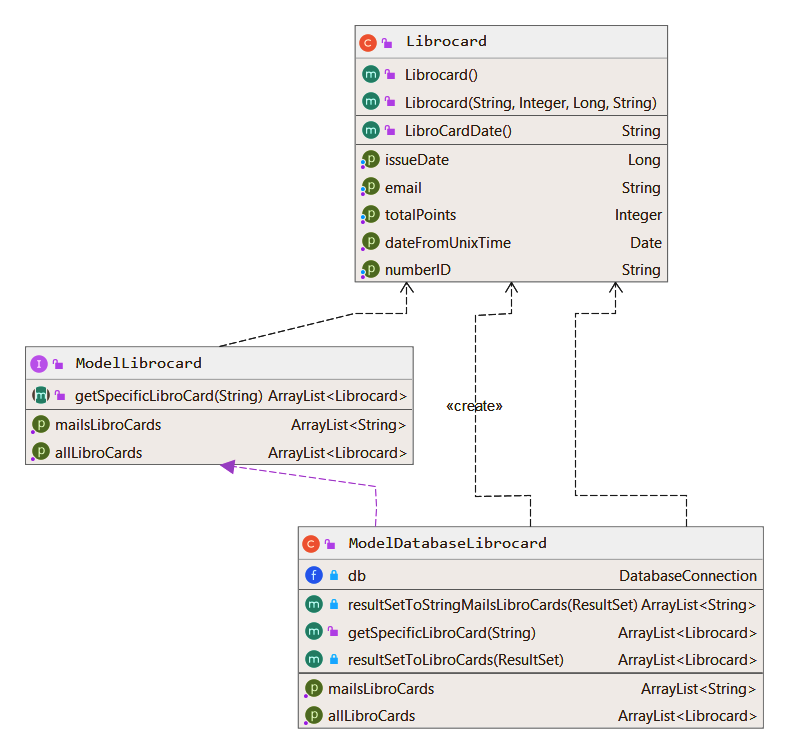
\includegraphics[width=1\linewidth]{Class diagrams/Librocard.png}
    	\caption{esempio implementazione DAO}
\end{figure} \leavevmode \\

La classe concreta ModelDatabaseLibroCard implementa l'interfaccia "dedicata" ModelLibroCard, la quale contiene solo i metodi inerenti alle LibroCards.

Notiamo che, se avessimo utilizzato i file come supporto di memorizzazione, allora la classe concreta in questione avrebbe dovuto utilizzare i metodi corretti per accedere al file, mantenendo però invariata la struttura delle prime due classi, quella \textit{entity} e quella \textit{Model interface}. È questo il principale \textbf{vantaggio} dell'utilizzo del pattern DAO: se si modifica il supporto di memorizzazione è necessario soltanto implementare una nuova classe concreta (per esempio \textit{ModelFileLibroCard}) che contiene i metodi per accedere alla nuova sorgente, senza però che le classi che si appoggiano ad essa cambino, o sappiano che tecnologia viene utilizzata.

\subsection{Singleton pattern}
Al fine di assicurare che la classe "DatabaseConnection" avesse una sola istanza ed un unico punto di accesso globale, questa è stata realizzata utilizzando il pattern singleton.\\
L'implementazione adottata è "lazy" ovvero l'istanza della classe viene creata solamente alla prima richiesta di utilizzo.\\

\subsection{Observer pattern}
Non abbiamo implementato un Observer da zero, ma abbiamo utilizzato quello messo a disposizione dalle librerie di JavaFX inerente ai listener dei buttoni, al fine di permettere la comunicazione tra View e Controller.\\
Abbiamo quindi i pulsanti delle varie View che sono gli observer, che stanno in ascolto e aspettano un determinato evento, in questo caso un click, e all'avvenimento dell'evento, una funzione di handler specifica per quel determinato bottone, va in esecuzione.\\

\subsection{Iterator pattern}
Anche in questo caso non abbiamo implementato un Iterator da zero ma abbiamo utilizzato quello messo a disposizione dalle librerie di Java.\\
In particolare è stato utilizzato per iterare su tutte le Collection utilizzate e per scorrere in maniera sequenziale i vari "result set" delle query effettuate al Database.

\clearpage

\chapter{Validazione e Test}

In questa parte ci siamo concentrati su due aspetti dettati dal test software: la verifica se l'applicativo raggiunge i risultati pianificati e la scoperta dei difetti. Per quanto riguarda l'ultimo caso, abbiamo forzato l'applicativo nei casi limite. \\
L'\textit{ispezione del software} è stata svolta in modo statico, ovvero senza l'avvio diretto del programma, e riguarda i requisiti utente discussi precedentemente, oltre alla pianificazione della base di dati. È stato dedicato più tempo al \textit{test software} dinamico, che comprende test di sviluppo, di rilascio e verso l'utente.
\newline
Nel \textbf{test di sviluppo} abbiamo effettuato test dei componenti e del sistema. In particolare, nel test dei componenti abbiamo testato le parti di codice che l'altra persona nel gruppo aveva scritto, e riguardava l'utilizzo delle interfacce, o il passaggio dei parametri. Il test di sistema è stato eseguito su tutto il programma da entrambi.
\newline
Il \textbf{test di rilascio} è stato eseguito da persone esterne, ma non ancora utenti finali, ovvero colleghi universitari tecnici, ma che non conoscevano com'era stato programmato il software.
\newline
Infine, nel \textbf{test utente} si sono coinvolti utenti finali, che nel nostro caso sono stati familiari e amici. È stato più precisamente un $\alpha$-test, in quanto è stato svolto sulle nostre macchine.

\section{Esempio caso d'uso - Ordine utente registrato}
Di seguito mostriamo un caso d'uso da parte di un utente registrato. \\All'avvio del programma si presenta la schermata iniziale.

\begin{figure}[h!]
	\centering
	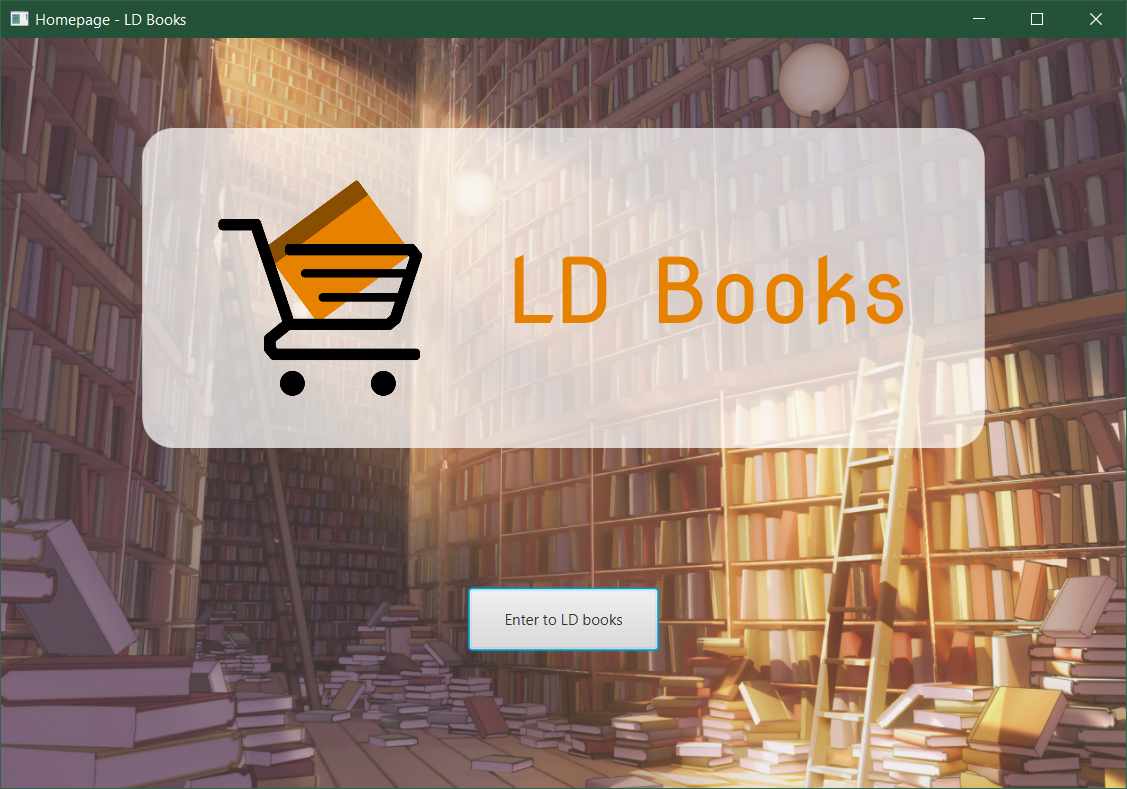
\includegraphics[width=0.8\linewidth]{Screenshots/homepage.png}
\end{figure}

Appena si clicca il bottone, si viene reindirizzati al catalogo dei libri. Qui è possibile filtrare per genere e/o lingua, oppure ricercare il titolo di un libro.

\begin{figure}[h!]
	\centering
	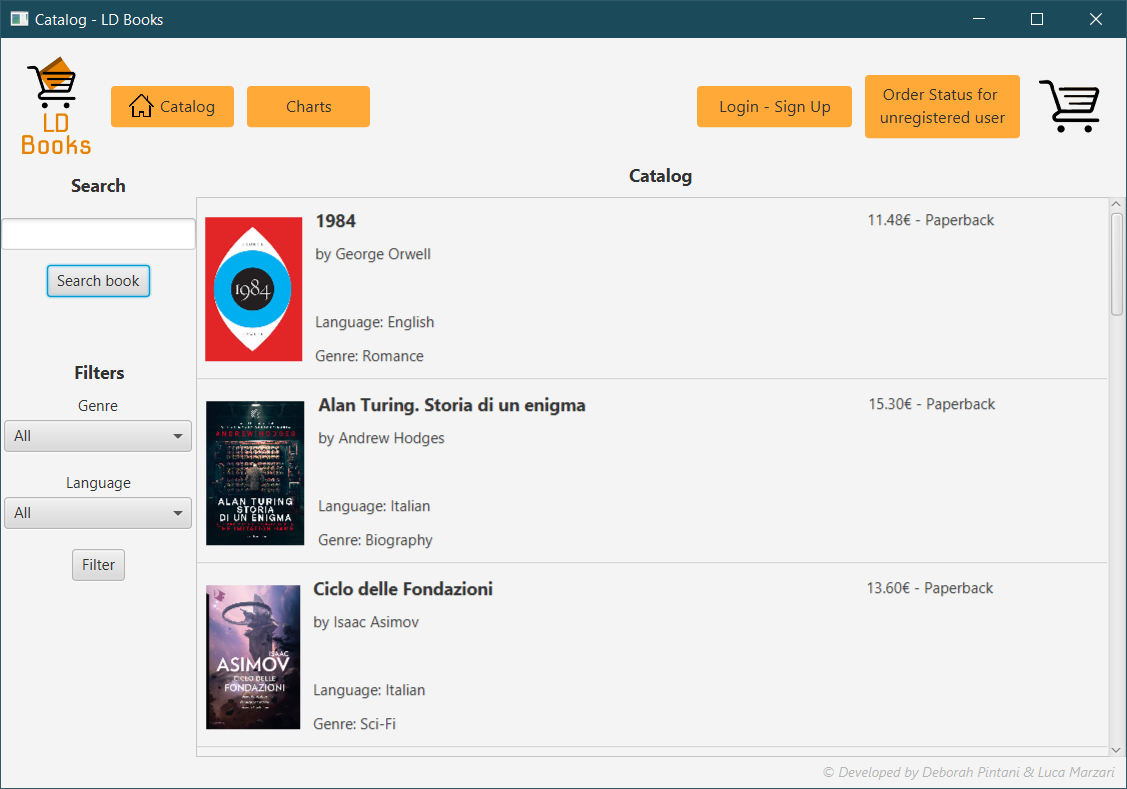
\includegraphics[width=0.8\linewidth]{Screenshots/catalogo.png}
\end{figure}
\newpage

\begin{figure}[h!]
	\centering
	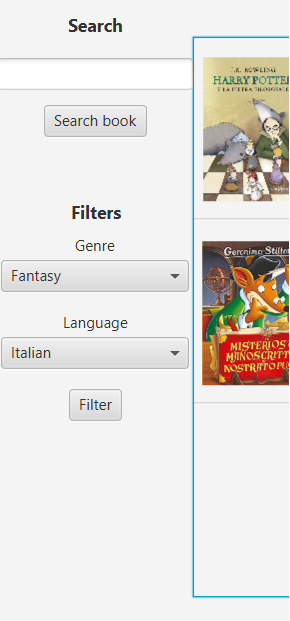
\includegraphics[width=0.3\linewidth]{Screenshots/filtroLibro.png}
\end{figure}

In qualsiasi caso, dopo aver filtrato o ricercato un libro, non appena si clicca su di esso è possibile visualizzare tutte le sue informazioni, comprese le varie tipologie di formati (copertina flessibile, rigida...) i quali sono raggruppati per libro.

\begin{figure}[h!]
	\centering
	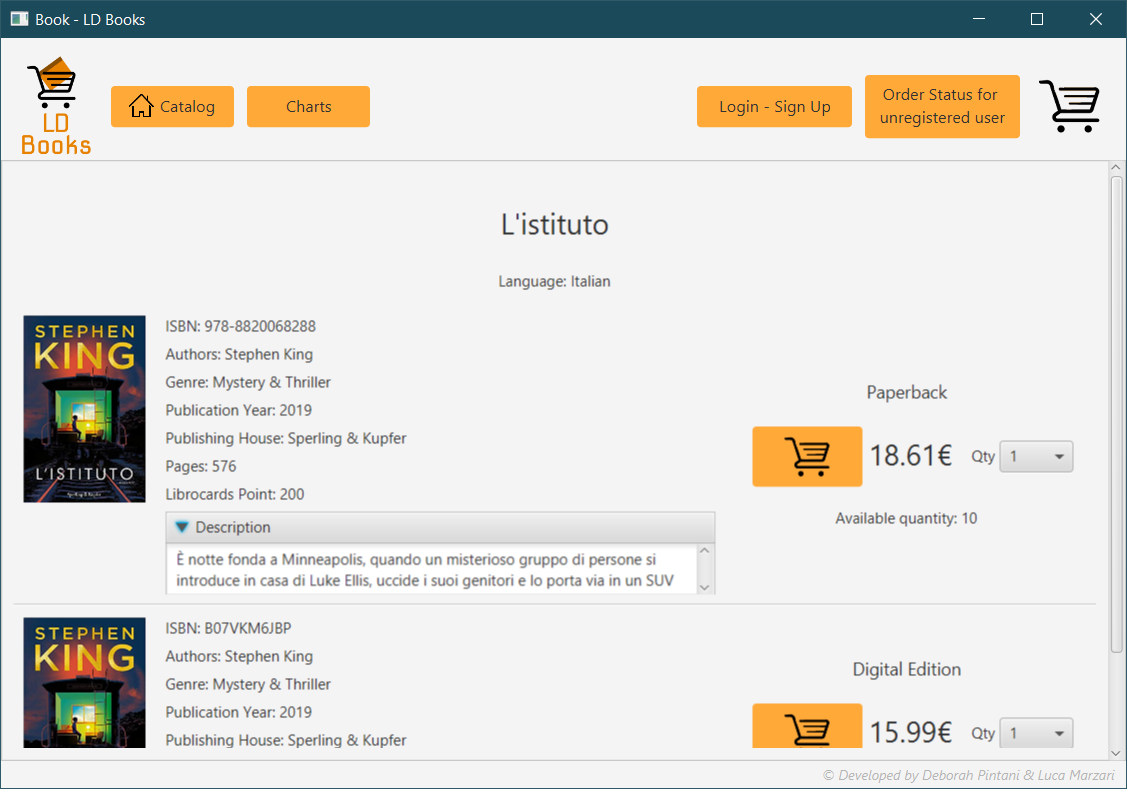
\includegraphics[width=0.8\linewidth]{Screenshots/libroSpecifico.png}
\end{figure}

Da questa pagina è possibile scegliere quante copie del libro acquistare dal menu a tendina, e successivamente metterle nel carrello premendo il pulsante accanto.
\newpage

\begin{figure}[h!]
	\centering
	\includegraphics[width=0.3\linewidth]{Screenshots/libroQuantità.png}
\end{figure}

\begin{figure}[h!]
	\centering
	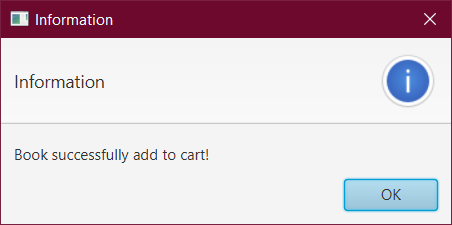
\includegraphics[width=0.5\linewidth]{Screenshots/libroAggiuntoCarrello.png}
\end{figure}

Se il libro non è disponibile perché non ci sono copie in magazzino, è mostrato un messaggio di errore.

\begin{figure}[h!]
	\centering
	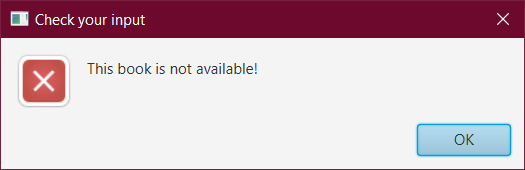
\includegraphics[width=0.5\linewidth]{Screenshots/libroNonDisp.png}
\end{figure}

Cliccando sul pulsante del carrello in alto a destra di ogni schermata, si accede al proprio carrello. Sono mostrati i dati riepilogativi dei libri e dell'eventuale ordine, con il prezzo totale, i punti LibroCard e la spedizione.
\newpage

\begin{figure}[h!]
	\centering
	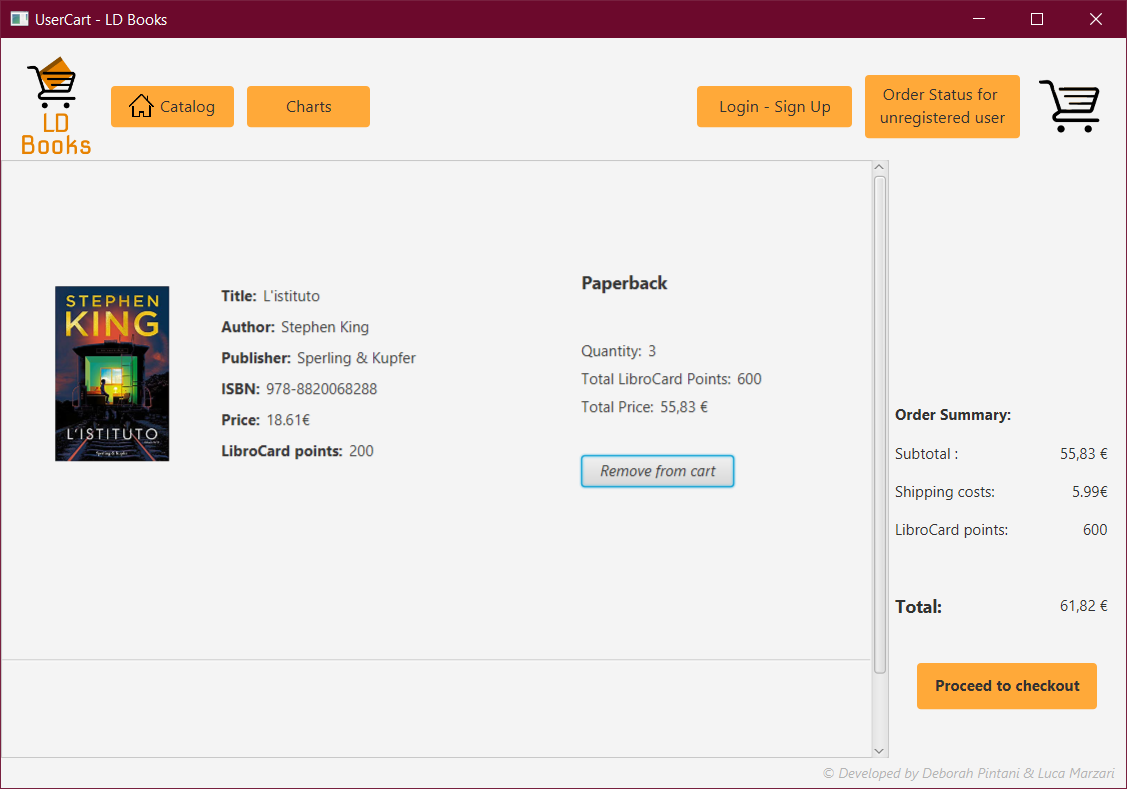
\includegraphics[width=0.8\linewidth]{Screenshots/carrello.png}
\end{figure}

È possibile rimuovere un libro dal carrello cliccando il pulsante "Remove from cart". Cliccando sul bottone "Proceed to checkout" si arriva alla schermata di Login nel caso questo non fosse stato effettuato precedentemente.

\begin{figure}[h!]
	\centering
	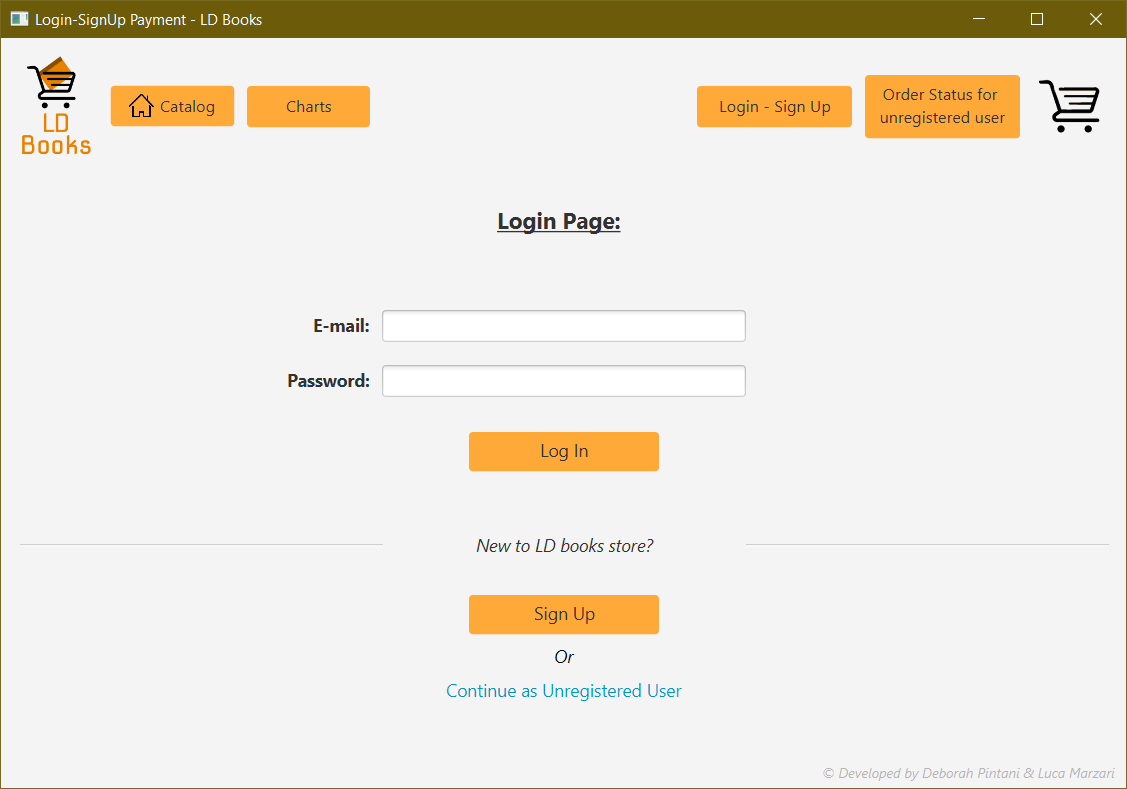
\includegraphics[width=0.8\linewidth]{Screenshots/login.png}
\end{figure}

L'utente può quindi autenticarsi se possiede un account, registrarsi se non lo possiede oppure continuare come utente non registrato. Stiamo discutendo un caso d'uso di un utente già registrato, perciò si esegue il login.\\
Se i dati inseriti non sono corretti, è mostrato un messaggio di errore.

\begin{figure}[h!]
	\centering
	\includegraphics[width=0.5\linewidth]{Screenshots/loginErrato.png}
\end{figure}
\newpage

Una volta effettuato l'accesso, si rimanda alla schermata di pagamento. Notiamo come anche l'header della schermata ci informi che siamo autenticati. È mostrato un riepilogo e si sceglie il tipo di pagamento e l'indirizzo al quale si desidera spedire.

\begin{figure}[h!]
	\centering
	\includegraphics[width=0.8\linewidth]{Screenshots/payment.png}
\end{figure}

Visto che entrambe le informazioni sono necessarie, se non vengono selezionate è mostrato un messaggio di errore.

\begin{figure}[h!]
	\centering
	\includegraphics[width=0.5\linewidth]{Screenshots/paymentErrore.png}
\end{figure}

Se l'ordine è andato a buon fine, allora è mostrato il seguente messaggio, con il codice dell'ordine.

\begin{figure}[h!]
    \centering
	\includegraphics[width=0.4\linewidth]{Screenshots/alertOrdine.png}
\end{figure}

\end{document}